\documentclass[cn,10pt,chinesefont=founder,math=newtx,cite=super,twoside]{elegantbook}

% 自定义封面
\makeatletter
\renewcommand{\maketitle}{%
	\pagenumbering{Alph}%
	\thispagestyle{empty}%
	\vspace*{5cm}%
	\begin{center}
		{\zihao{1}\heiti\@title}\\[28pt]
		\@author
	\end{center}
}
\makeatother
\title{光学与光子学}
\author{\Large{关其锐\hspace{\ccwd}{\heiti 著}}}

%\title{光学与光子学}
%\subtitle{专业课学习笔记}

%\author{Keiyui Kwan}
%\institute{Zhejiang University}
%\date{\today}
%\version{1.00}
%\bioinfo{自定义}{信息}

%\extrainfo{God said, "Let there be light", and there was light.}

%\logo{logo.png}
%\cover{cover.jpg}

% 修改目录深度
\setcounter{tocdepth}{2}

%*********************
\usetikzlibrary{intersections}
\usetikzlibrary{quotes,angles}
\usetikzlibrary{patterns}
\tikzstyle{every picture}+=[remember picture]

%\everymath{\displaystyle}

\usepackage{tasks} %选择题宏包,tasks环境

% 选择题示例 
%\begin{tasks}(4)
%	\task 
%	\task 
%	\task 
%	\task 
%\end{tasks}

% 表格内分行
\newcommand{\tabincell}[2]{\begin{tabular}{@{}#1@{}}#2\end{tabular}}

% 批注
\definecolor{tcolor}{RGB}{255,127,  0} % default: 0,124,53
\definecolor{lcolor}{RGB}{255,178,102} % default: 153,255,153
\definecolor{pcolor}{RGB}{224,250,255} % default: 216,255,216

\newcommand{\elegantpar}[2]{%
	\textcolor{tcolor}{$\bm\langle{}\!{}$#1${}\!{}\bm\rangle$}%
	\begin{tikzpicture}[remember picture, baseline=-0.75ex]%
	\node[coordinate] (inText) {};%
	\end{tikzpicture}%
	\marginpar{%
		\renewcommand{\baselinestretch}{1.0}%
		\begin{tikzpicture}[remember picture]%
		\draw node[fill= pcolor, rounded corners,text width=\marginparwidth] (inNote){\footnotesize#2};%
		\end{tikzpicture}%
	}%
	\begin{tikzpicture}[remember picture, overlay]%
	\draw[draw = lcolor, thick]
	([yshift=-0.55em] inText)
	-| ([xshift=-0.55em] inNote.west)
	-| (inNote.west);%
	\end{tikzpicture}%
}
%*********************

\begin{document}
	
\maketitle
\frontmatter
	
\chapter*{前言}
\markboth{前言}{introduction}
欢迎您阅读本书。在2019年末,我顺利完成了本科光电专业必修理论知识的学习。为了方便查阅光学方面的各种基本概念,复习巩固光学基础知识,我便开始计划写下本书。本书进行书写时参考的资料主要为国内光电专业通用的课程教材:郁道银等编著的《工程光学(第四版)》和李晓彤等编著的《几何光学·像差·光学设计(第三版)》。我将本书看作是一本工具书,我对这本工具书的要求是,文字内容源于教材但要凝练,读者能够方便查阅相关概念,配图要精美,排版要美观。文字内容方面,因为本书的面向对象是光电专业的读者,因此对于一些简单的光学概念本书不再进行原理分析,本书重点突出了一些我认为需要重点掌握和易错的知识点。为了方便查阅,本书对光学概念分章节进行汇总,并设有目录,文中的图表、公式都设有标签可以进行跳转。配图方面,本书尽可能多地使用矢量图,这些矢量图来自维基百科和我自己的绘制。但因为我的时间有限,仍有较多图片使用了教材中的截图。对于本书的排版,我采用了\LaTeX 进行写作,模板采用的是Elegant\LaTeX 系列模板中的 \href{https://github.com/ElegantLaTeX/ElegantBook}{ElegantBook}。本书为免费共享书籍,请勿用于商业用途。

\tableofcontents
\mainmatter

\part{应用光学}

\chapter{几何光学基本概念与定律}

\begin{introduction}
	\item 可见光波长(表 \ref{tab:visible-light})
	\item 四个基本定律(第 \ref{subsect:basic-law} 节)
	\item 全反射(定义 \ref{def:total-internal-reflection})
	\item 费马原理(命题 \ref{pro:fermats-principle})
\end{introduction}

\section{基本定律和原理}

\subsection{光波与光线}
光波波长的范围大致为$1\mathrm{mm}$至$10\mathrm{nm}$,其中可见光波段为$380\mathrm{nm}$至$780\mathrm{nm}$之间,不同颜色对应的波段参考范围如\tabref{tab:visible-light} 所示。光波在真空中的传播速度为$c\approx 2.9979\times 10^8\mathrm{m/s}$。

\begin{table}[htbp]
	\small
	\caption{可见光不同颜色对应的波段参考范围\label{tab:visible-light}}
	\centering
	\begin{tabular}{cccccccc}
		\toprule
		&\color{red}{红色}&\color{orange}{橙色}&\color{yellow}{黄色}&\color{green}{绿色}&\color{cyan}{青色}&\color{blue}{蓝色}&\color{violet}{紫色}\\
		\midrule
		$\lambda$(nm)&$780\sim620$&$620\sim590$&$590\sim570$&$570\sim495$&$495\sim476$&$476\sim450$&$450\sim380$\\
		\bottomrule
	\end{tabular}
\end{table}

\subsection{基本定律}
\label{subsect:basic-law}
光线传播遵循以下四个基本定律:
\begin{enumerate}
	\item 直线传播定律:在各向同性的均匀介质中,光在两点之间沿直线传播,即在这种介质中,光线都是直线。
	\item 独立传播定律:以不同途径传播的光同时在空间某点通过时,彼此互不影响,各路光独立传播,在各光路相遇处,其光强度是简单地相加,总是增强的。
	\item 反射定律:反射光线与入射光线和法线在同一平面内,入射光线和反射光线分别位于法线的两侧,与法线的夹角相同,即
	\begin{equation}
	I''=-I
	\end{equation}
	\item 折射定律:折射光线与入射光线和法线在同一平面内,折射角与入射角的正弦之比与入射角的大小无关,仅由两介质的性质决定。即有
	\begin{equation}
	n'\sin I'=n\sin I
	\end{equation}
\end{enumerate}

\begin{note}
	光的直线传播定律和独立传播定律只有在不考虑光的波动性质时才是正确的。反射定律可以认为是折射定律在$n'=-n$时的特殊情况。
\end{note}

\begin{definition}{全反射}{total-internal-reflection}
	如\figref{fig:total-internal-reflection} 所示,当光线由光密介质向光疏介质传播时,因$n'<n$,则折射角$I'$小于入射角$I$,折射光线远离法线。逐渐增大入射角$I$至某一个值,折射角$I'$达到$90^{\circ}$,折射光线沿界面掠出。若入射角继续增大,则无出射光线存在,全部返回原介质内,达到全反射。其中,临界角$I_m$有
	\begin{equation}
	\sin I_m=\frac{n'}{n}
	\end{equation}
\end{definition}

\begin{figure}[htbp]
	\centering
	\begin{tikzpicture}
	% define coordinates
	\coordinate (A) at (-3,-3);
	\coordinate (B) at (-1.5,0);
	\coordinate (C) at (-1.5,-1.5);
	\coordinate (D) at (-1.5,1.5);
	\coordinate (E) at (0,1.8);
	\coordinate (F) at (0,0);
	\coordinate (G) at (0,-1.5);
	\coordinate (H) at (1.5,0);
	% media
	\fill[blue!25!,opacity=.3] (-4,0) rectangle (4,2);
	\fill[blue!60!,opacity=.3] (-4,0) rectangle (4,-3.5);
	\node[left] at (-3,-3) {光源};
	\node[above] at (-3.5,0) {$n_2$};
	\node[below] at (-3.5,0) {$n_1$};
	\node[above left] at (3,0) {全反射};
	% axis
	\draw[dash pattern=on5pt off3pt,red] (-1.5,-1.5) -- (-1.5,1.5);
	\draw[dash pattern=on5pt off3pt,red] (0,-1.5) -- (0,1.5);
	\draw[dash pattern=on5pt off3pt,red] (3,-1.5) -- (3,1.5);
	% rays
	\draw[blue,-latex] (-3,-3) -- (-3,0);
	\draw[blue,-latex] (-3,0) -- (-3,1.8);
	
	\draw[blue,-latex] (-3,-3) -- (-1.5,0);
	\draw[blue,-latex] (-1.5,0) -- (0,1.8);
	\draw[cyan,-latex] (-1.5,0) -- (0,-3);
	
	\draw[blue,-latex] (-3,-3) -- (0,0);
	\draw[blue,-latex] (0,0) -- (1.5,0);
	\draw[cyan,-latex] (0,0) -- (3,-3);
	
	\draw[blue,-latex] (-3,-3) -- (3,0);
	\draw[blue,-latex] (3,0) -- (3.5,-0.25);
	% angles
	\pic["$\theta_1$", draw=black, -, angle eccentricity=1.6, angle radius=0.5cm]{angle=A--B--C};
	\pic["$\theta_2$", draw=black, -, angle eccentricity=1.6, angle radius=0.5cm]{angle=E--B--D};
	\pic["$\theta_c$", draw=black, -, angle eccentricity=1.6, angle radius=0.5cm]{angle=A--F--G};
	\pic["$90^{\circ}$", draw=black, -, angle eccentricity=1.8, angle radius=0.4cm]{angle=H--F--E};
	\end{tikzpicture}
	\caption{全反射示意图}
	\label{fig:total-internal-reflection}
\end{figure}

\begin{problem}
	若水面下$200\mathrm{mm}$处有一发光点,水的折射率为$4/3$,求在水面上能看到被该发光点照亮的范围有多大?
	\begin{tasks}(4)
		\task $453.56\mathrm{mm}$
		\task $226.79\mathrm{mm}$
		\task $352.77\mathrm{mm}$
		\task $176.38\mathrm{mm}$
	\end{tasks}
\end{problem}
\begin{solution}
	选择a。由全反射的定义可知光从水中到空气中传播是临界角为
	\begin{equation}
	\sin I_m=\frac{n'}{n}=\frac{1}{4/3}=0.75\notag
	\end{equation}
	可得$I_m=48.59^{\circ}$,$\tan I_m=1.13389$,由几何关系可得被该发光点照亮的范围是
	\begin{equation}
	2\times200\times1.13389=453.6(\mathrm{mm})\notag
	\end{equation}
\end{solution}

\begin{problem}
	已知光在真空中的传播速度为$3\times10^8\mathrm{m/s}$,求光在折射率为$1.333$的水中和$1.65$的玻璃中的传播速度。
\end{problem}
\begin{solution}
	由$n=c/v$可得,光在水中的传播速度为
	\begin{equation}
	v_{\mathrm{water}}=\frac{c}{n_{\mathrm{water}}}=\frac{3\times10^8}{1.333}=2.25(\mathrm{m/s})\notag
	\end{equation}
	光在玻璃中的传播速度为
	\begin{equation}
	v_{\mathrm{glass}}=\frac{c}{n_{\mathrm{glass}}}=\frac{3\times10^8}{1.65}=1.818(\mathrm{m/s})\notag
	\end{equation}
\end{solution}

\begin{problem}
	以高度为$1.7\mathrm{m}$的人立于离高度为$5$米的路灯$1.5\mathrm{m}$处,求其影子的长度。
\end{problem}
\begin{solution}
	根据光的直线传播定律,设其影子长为$x$,则有
	\begin{equation}
	\frac{1.7}{5}=\frac{x}{1.5+x}\notag
	\end{equation}
	可得$x=0.773\mathrm{m}$。
\end{solution}

\begin{problem}
	一针孔照相机对一物体于屏上形成一$60\mathrm{mm}$高的像,若将屏拉远$50\mathrm{mm}$,则像的高度为$70\mathrm{mm}$。试求针孔到屏间的原始距离。
\end{problem}
\begin{solution}
	根据光的直线传播定律,设针孔到屏间的原始距离为$x$,则有
	\begin{equation}
	\frac{70}{50+x}=\frac{60}{x}\notag
	\end{equation}
	可得$x=300\mathrm{mm}$。
\end{solution}

\begin{problem}
	有一光线以$60^{\circ}$的入射角入射于$n=\sqrt{3}$的磨光玻璃球上的任一点,其折射光线继续传播到球表面的另一点上,求在该点反射和折射的光线间夹角。
\end{problem}
\begin{solution}
	根据光的反射定律
	\begin{equation}
	I''=-I\notag
	\end{equation}
	得到反射角为$I''=60^{\circ}$,由折射定律
	\begin{equation}
	n'\sin I'=n\sin I\notag
	\end{equation}
	得到折射角$I'=30^{\circ}$,由几何关系可得该点反射和折射光线的夹角为$90^{\circ}$。
\end{solution}

\begin{remark}
折射定律和反射定律可用矢量形式进行计算。
\end{remark}

\begin{figure}[htbp]
	\centering
	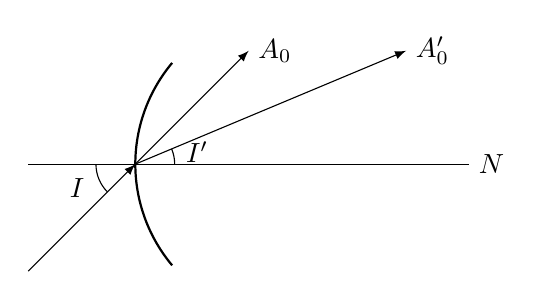
\begin{tikzpicture}[scale=0.8] 
	\coordinate (A) at (-1.3,0);
	\coordinate [label=right:$\boldsymbol{A}_0$] (B) at (0.5,1.8);
	\coordinate [label=right:$\boldsymbol{A}'_0$] (C) at (3,1.8);
	\coordinate [label=right:$\boldsymbol{N}$] (D) at (4,0);
	\coordinate (E) at (-3,0);
	\coordinate (F) at (-3,-1.7);
	\draw[-] (-3,0) -- (4,0); 
	\draw[-latex] (-3,-1.7) -- (A); 
	\draw[-latex] (A) -- (B);
	\draw[-latex] (A) -- (3,1.8);
	\draw[line width=0.8pt] (A) arc (180:220:2.5);
	\draw[line width=0.8pt] (A) arc (180:140:2.5);
	\pic["$I$", draw=black, -, angle eccentricity=1.6, angle radius=0.5cm]{angle=E--A--F};
	\pic["$I'$", draw=black, -, angle eccentricity=1.6, angle radius=0.5cm]{angle=D--A--C};
	\end{tikzpicture}
	\caption{光线的矢量形式}
	\label{fig:vector-light}
\end{figure}

如\figref{fig:vector-light} 所示,$\boldsymbol{A}_0$和$\boldsymbol{A}'_0$分别是沿入射光线和折射光线的单位矢量,$\boldsymbol{N}$是沿法线的单位矢量。法线矢量的方向是从入射介质到折射介质。按此,光的折射定律公式可写为
\begin{equation}
n'(\boldsymbol{A}'_0\times\boldsymbol{N})=n(\boldsymbol{A}_0\times\boldsymbol{N}')
\end{equation}
展开上式,并将长度为$n'$的折射光线和长度为$n$的入射光线矢量分别记为$\boldsymbol{A}'$和$\boldsymbol{A}$,得
\begin{equation}
\boldsymbol{A}'\times\boldsymbol{N}=\boldsymbol{A}'\times\boldsymbol{N}
\end{equation}
\begin{equation}
(\boldsymbol{A}'-\boldsymbol{A})\times\boldsymbol{N}=0
\end{equation}
$(\boldsymbol{A}'-\boldsymbol{A})$和$\boldsymbol{N}$都不可能为零,因此,两矢量必定是互相平行的,所以上式可表示为
\begin{equation}
\boldsymbol{A}'-\boldsymbol{A}=P\boldsymbol{N}=0
\end{equation}
上式两边都与$\boldsymbol{N}$作标积,得
\begin{equation}
P=\boldsymbol{N}\cdot\boldsymbol{A}'-\boldsymbol{N}\cdot\boldsymbol{A}=n'\cos I'-n\cos I
\end{equation}
当$n'>n$时,$P>0$,$(\boldsymbol{A}'-\boldsymbol{A})$与$\boldsymbol{N}$正向平行,反之,两矢量反向平行。一般情况下,在已知两介质折射率和光线入射角求折射角时,$P$可化为
\begin{equation}
P=\sqrt{n'^2-n^2+n^2\cos^2 I}-n\cos I
\end{equation}
\begin{equation}
\boldsymbol{A}'=\boldsymbol{A}+P\boldsymbol{N}
\end{equation}
上式即为矢量形式的折射定律。
在$n'=-n$的情况下,有
\begin{equation}
P=n'\cos I'-n\cos I=-2n\cos I=-2(\boldsymbol{N}\cdot\boldsymbol{A})
\end{equation}
得到
\begin{equation}
\boldsymbol{A}''=\boldsymbol{A}-2\boldsymbol{N}(\boldsymbol{N}\cdot\boldsymbol{A})
\end{equation}
上式即为矢量形式的反射定律。

\begin{problem}
	有一光线$\boldsymbol{A}=\cos 60^{\circ}\boldsymbol{i}+\cos 30^{\circ}\boldsymbol{j}$入射于$n=1$和$n'=1.5$的平面分界面上,平面的法线为$\boldsymbol{N}=\cos 30^{\circ}\boldsymbol{i}+\cos 60^{\circ}\boldsymbol{j}$,求反射光线$\boldsymbol{A}''$和折射光线$\boldsymbol{A}'$。
\end{problem}
\begin{solution}
	由
	\begin{equation}
	\boldsymbol{N}\cdot\boldsymbol{A}=n\cos I\notag
	\end{equation}
	得到
	\begin{equation}
	(\cos 60^{\circ}\boldsymbol{i}+\cos 30^{\circ}\boldsymbol{j})(\cos 30^{\circ}\boldsymbol{i}+\cos 60^{\circ}\boldsymbol{j})=\frac{\sqrt{3}}{2}=\cos I\notag
	\end{equation}
	所以有
	\begin{equation}
	\begin{aligned}
	P&=\sqrt{n'^2-n^2+n^2\cos^2 I}-n\cos I\\
	&=\sqrt{1.5^2-1+\bigg(\frac{\sqrt{3}}{2}\bigg)^2}-1\times\frac{\sqrt{3}}{2}\\
	&=\sqrt{2}-\frac{\sqrt{3}}{2}\notag
	\end{aligned}
	\end{equation}
	所以由矢量形式的折射定律得
	\begin{equation}
	\begin{aligned}
	\boldsymbol{A}'&=\boldsymbol{A}+P\boldsymbol{N}\\
	&=(\cos 60^{\circ}\boldsymbol{i}+\cos 30^{\circ}\boldsymbol{j})+\bigg(\sqrt{2}-\frac{\sqrt{3}}{2}\bigg)(\cos 30^{\circ}\boldsymbol{i}+\cos 60^{\circ}\boldsymbol{j})\\
	&=\bigg(\frac{2\sqrt{6}-1}{4}\bigg)\boldsymbol{i}+\bigg(\frac{2\sqrt{2}+\sqrt{3}}{4}\bigg)\boldsymbol{j}\notag
	\end{aligned}
	\end{equation}
	所以由矢量形式的反射定律得
	\begin{equation}
	\begin{aligned}
	\boldsymbol{A}''&=\boldsymbol{A}-2\boldsymbol{N}(\boldsymbol{N}\cdot\boldsymbol{A})\\
	&=(\cos 60^{\circ}\boldsymbol{i}+\cos 30^{\circ}\boldsymbol{j})-2(\cos 30^{\circ}\boldsymbol{i}+\cos 60^{\circ}\boldsymbol{j})[(\cos 60^{\circ}\boldsymbol{i}+\cos 30^{\circ}\boldsymbol{j})\cdot(\cos 30^{\circ}\boldsymbol{i}+\cos 60^{\circ}\boldsymbol{j})]\\
	&=-\boldsymbol{i}\notag
	\end{aligned}
	\end{equation}
\end{solution}

\subsection{费马原理}

\begin{proposition}{费马原理}{fermats-principle}
	光从一点到另一点是沿光程为极值的路径传播的。即光沿光程为极小、极大或常量的路径传播,又称为极端光路定律。
\end{proposition}

如\figref{fig:fermats-principle} 所示,光从空气射入水中,从$A$点到$B$点,途径$P$点,其光路$APB$为光传播时间最短的路径。 

\begin{figure}[htbp]
	\centering
	\begin{tikzpicture}[scale=0.6] 
	% define coordinates
	\coordinate [label=below left:$P$] (O) at (0,0);
	\coordinate (A) at (0,4);
	\coordinate (B) at (0,-4);
	\coordinate [label=below left:$A$] (C) at (-3.2,4);
	\coordinate [label=above left:$B$] (D) at (2.2,-4);
	% media
	\fill[blue!25!,opacity=.3] (-4,0) rectangle (4,4);
	\fill[blue!60!,opacity=.3] (-4,0) rectangle (4,-4);
	\node[right] at (2,2) {空气};
	\node[left] at (-2,-2) {水};
	% axis
	\draw[dash pattern=on5pt off3pt] (A) -- (B);
	% rays
	\draw[red,latex-] (O) -- (130:5.2);
	\draw[blue,-latex] (O) -- (-70:4.24);
	% angles
	\draw (0,1) arc (90:130:1);
	\draw (0,-1.4) arc (270:290:1.4);
	\node[] at (280:1.8)  {$\theta_{2}$};
	\node[] at (110:1.4)  {$\theta_{1}$};
	\end{tikzpicture}
	\caption{费马原理演示}
	\label{fig:fermats-principle}
\end{figure}

\section{完善成像}
完善成像条件:物点与像点之间任意两条的光路光程相等。

\chapter{球面与球面系统}

\begin{introduction}
	\item 符号规则(第 \ref{sect:symbol-rules} 节)
	\item 近轴光线光路(第 \ref{sect:paraxial-ray} 节)
	\item 三种放大率(第 \ref{sect:three-magnification} 节)
\end{introduction}

\section{概念与符号规则}
\label{sect:symbol-rules}
\figref{fig:spherical-system} 所示的是光线经球面折射的光路。对于单个球面,凡过球心的直线就是其光轴,包含光轴的平面为子午平面,光轴与球面的交点称为顶点。$L$为物方截距,$U$为物方倾斜角;。$L'$为像方截距,$U'$为像方倾斜角。

\begin{figure}[htbp]
	\centering
	\begin{tikzpicture} 
	\coordinate [label=below left:$A$] (A) at (-4,0);
	\coordinate [label=below right:$A'$] (B) at (3.8,0);
	\coordinate [label=below:$C$] (C) at (0.8,0);
	\coordinate [label=below left:$O$] (D) at (-1.3,0);
	\coordinate [label=above:$E$] (E) at (-1,1.2);
	\coordinate (F) at (-9/5,26/15);
	\draw[-] (-5,0) -- (5,0); 
	\draw[red,-latex] (A) -- (E);
	\draw[red,-latex] (E) -- (B); 
	\draw[-] (C) -- (F); 
	\draw[line width=0.8pt] (D) arc (180:220:2.5);
	\draw[line width=0.8pt] (D) arc (180:140:2.5);
	\pic["$-U$", draw=black, -latex, angle eccentricity=1.6, angle radius=0.8cm]
	{angle=D--A--E};%\alpha的位置由eccentricity决定。
	\pic["$U'$", draw=black, latex-, angle eccentricity=1.3, angle radius=1cm]
	{angle=E--B--D};
	\pic["$\varphi$", draw=black, -, angle eccentricity=1.3, angle radius=0.5cm]
	{angle=E--C--D};
	\pic["$I'$", draw=black, latex-, angle eccentricity=1.6, angle radius=0.8cm]
	{angle=C--E--B};
	\pic["$I$", draw=black, latex-, angle eccentricity=1.6, angle radius=0.5cm]
	{angle=F--E--A};
	\draw[latex-latex] (E) -- ($(A)!(E)!(C)$)node[black,midway,xshift=0.2cm]{$h$};
	\coordinate [label=below:$n$] (m) at (-2,-1);
	\coordinate [label=below:$n'$] (n) at (0,-1);
	\coordinate [label=below:$r$] (r) at (-0.5,-0.1);
	\draw (-4,-2) -- ($(A)!(-4,-2)!(C)$);
	\draw (-1.3,-2) -- ($(A)!(-1.3,-2)!(C)$);
	\draw (3.8,-2) -- ($(A)!(3.8,-2)!(C)$);
	\draw[latex-latex](-4,-1.8) -- (-1.3,-1.8) node[black,below,midway](line){$-L$};
	\draw[latex-latex](3.8,-1.8) -- (-1.3,-1.8) node[black,below,midway](line){$L'$};
	\end{tikzpicture}
	\caption{光线经球面折射的光路}
	\label{fig:spherical-system}
\end{figure}

符号规则:
\begin{enumerate}
	\item 沿轴线段:如$L$、$L'$和$r$,以界面顶点为原点,如果由原点到光线与光轴的交点和到球心的方向与光线传播方向相同,其值为正,反之为负。光线传播方向规定自左向右。
	\item 垂轴线段:如$h$,在光轴之上为正,之下为负。
	\item 光线与光轴的夹角$U$和$U'$:以光轴为始边,从锐角方向转到光线,顺时针为正,逆时针为负。
	\item 光线与法线的夹角$I$、$I'$和$I''$:以光线为始边,从锐角方向转到法线,顺时针为正,逆时针为负。
	\item 表面间隔$d$:有前一面的顶点到后一面的顶点,其方向与光线方向相同者为正,反之为负,在纯折射系统中,$d$恒为正。
\end{enumerate}

\section{轴上物点经单个折射球面成像}
\label{sect:paraxial-ray}
由\figref{fig:spherical-system} 可得
\begin{equation}
\varphi=U+I=U'+I'
\end{equation}
结合折射定律,可导出
\begin{equation}
\sin I=\frac{L-r}{r}\sin U
\end{equation}
\begin{equation}
\sin I'=\frac{n}{n'}\sin I
\end{equation}
\begin{equation}
U'=U+I-I'
\end{equation}
\begin{equation}
L'=r+r\frac{\sin I'}{\sin U'}
\end{equation}
如果入射光线与光轴的夹角很小,则称之为近轴光线。近轴光线的有关量用小写字母表示,则有
\begin{equation}
i=\frac{l-r}{r}u
\end{equation}
\begin{equation}
i'=\frac{n}{n'}i
\end{equation}
\begin{equation}
u'=u+i-i'
\end{equation}
\begin{equation}
l'=r+r\frac{i'}{u'}
\end{equation}
近轴光线所成的像称为高斯像,讨论近轴区成像性质和规律的光学称为高斯光学。\index{高斯光学}

在以上公式中消去$i$和$i'$,并引入对近轴光线成立的简单关系
\begin{equation}
h=lu=l'u'
\end{equation}
可得
\begin{equation}
n'\bigg(\frac{1}{r}-\frac{1}{l'}\bigg)=n\bigg(\frac{1}{r}-\frac{1}{l}\bigg)=Q
\end{equation}
\begin{equation}
\frac{n'}{l'}-\frac{n}{l}=\frac{n'-n}{r}
\label{eq:spherical-refraction}
\end{equation}
\begin{equation}
n'u'-nu=\frac{n'-n}{r}h
\end{equation}

以上三式为同一公式的三种不同表示形式。$Q$为阿贝不变量。当物点位置一定时,一个球面的物空间和像空间的$Q$值相等。由式(\ref{eq:spherical-refraction})可见,对于给定物距$l$的物点,像的位置仅与$(n'-n)/r$有关,称之为折射球面的光焦度$\varphi$,有
\begin{equation}
\varphi=\frac{n'-n}{r}
\end{equation}
将$l=-\infty$和$l'=\infty$带入式(\ref{eq:spherical-refraction}),可得
\begin{equation}
f'=\frac{n'}{n'-n}r
\label{eq:spherical-image-focal-length}
\end{equation}
\begin{equation}
f=-\frac{n}{n'-n}r
\label{eq:spherical-object-focal-length}
\end{equation}
根据以上三式,折射球面的光焦度和焦距之间有如下关系:
\begin{equation}
\varphi=\frac{n'}{f'}=-\frac{n}{f}
\end{equation}
\begin{equation}
\frac{f'}{n'}=-\frac{f}{n}
\end{equation}
\begin{equation}
f'+f=r
\end{equation}

\begin{problem}
	有一直径为$100\mathrm{mm}$、折射率为$1.5$的抛光玻璃球,在视线方向可见球内有两个气泡,一个位于球心,另一个位于球心与前表面间的一半处。求两个气泡在球内的实际位置。
\end{problem}
\begin{solution}
	单折射面在近轴区域的物像关系公式为
	\begin{equation}
	\frac{n'}{l'}-\frac{n}{l}=\frac{n'-n}{r}
	\end{equation}
	球心的像,即有$l'=r$,所以
	\begin{equation}
	\frac{n}{l_1}=\frac{n'}{r}-\frac{n'-n}{r}=\frac{n}{r}
	\end{equation}
	即$l_1=r$,仍在球心,物像重合。
	
	另一个像,有$l'=r/2$,所以
	\begin{equation}
	\frac{n}{l_2}=\frac{n'}{r/2}-\frac{n'-n}{r}=\frac{n'+n}{r}
	\end{equation}
	\begin{equation}
	l_2=\frac{nr}{n'+n}=\frac{nD}{2(n'+n)}=20
	\end{equation}
	即距离前表面$30\mathrm{mm}$。
\end{solution}

\begin{problem}
	一折射球面,其像方焦距和物方焦距分别为$144\mathrm{mm}$和$-120\mathrm{mm}$,物方介质为$n=4/3$的水,求球面的曲率半径$r$和像方介质折射率$n'$。
	\begin{tasks}(2)
		\task $r=24\mathrm{mm}$,$n'=1.6$
		\task $r=-24\mathrm{mm}$,$n'=1.6$
		\task $r=24\mathrm{mm}$,$n'=1.11$
		\task $r=-24\mathrm{mm}$,$n'=1.11$
	\end{tasks}
\end{problem}
\begin{solution}
	选择a。由已知可得,$f=-120$,$f'=144$,$n=4/3$。根据公式
	\begin{equation}
	\frac{f'}{n'}=-\frac{f}{n}
	\end{equation}
	可得$n'=-\dfrac{f'\cdot n}{f}=-\dfrac{144\cdot 4/3}{-120}=1.6$
	
	由公式
	\begin{equation}
	f'+f=r
	\end{equation}
	得到半径为$r=f'+f=180-150=30\mathrm{mm}$。
\end{solution}

\section{物平面细光束经折射球面成像}
\label{sect:three-magnification}
由\figref{fig:imaging-magnification} 可得,横向放大率为
\begin{equation}
\beta=\frac{y'}{y}=\frac{l'-r}{l-r}=\frac{nl'}{n'l}
\end{equation}
轴向放大率为
\begin{equation}
\alpha=\frac{\mathrm{d}l'}{\mathrm{d}l}=\frac{nl'^2}{n'l^2}=\frac{n'}{n}\beta^2
\end{equation}
角放大率为
\begin{equation}
\gamma=\frac{u'}{u}=\frac{l}{l'}=\frac{n}{n'}\frac{1}{\beta}
\end{equation}
拉赫公式为
\begin{equation}
nyu=n'y'u'=J
\end{equation}
其中,$J$为拉赫不变量。

\begin{figure}[htbp]
	\centering
	\begin{tikzpicture} 
	\coordinate [label=below left:$A$] (A) at (-4,0);
	\coordinate [label=below right:$A'$] (B) at (3.8,0);
	\coordinate [label=below:$C$] (C) at (0.8,0);
	\coordinate [label=below left:$O$] (D) at (-1.3,0);
	\coordinate [label=above:$E$] (E) at (-1,1.2);
	\coordinate [label=left:$B$] (G) at (-4,1.2);
	\coordinate [label=right:$B'$] (H) at (3.8,-0.75);
	\draw[-] (-5,0) -- (5,0); 
	\draw[red,-latex] (A) -- (E);
	\draw[red,-latex] (E) -- (B); 	
	\draw[red,-latex] (G) -- (H);
	\draw[line width=0.8pt] (D) arc (180:220:2.5);
	\draw[line width=0.8pt] (D) arc (180:140:2.5);
	\pic["$-u$", draw=black, -latex, angle eccentricity=1.6, angle radius=0.8cm]
	{angle=D--A--E};
	\pic["$u'$", draw=black, latex-, angle eccentricity=1.3, angle radius=1cm]
	{angle=E--B--D};
	\draw[latex-latex] (E) -- ($(A)!(E)!(C)$)node[black,midway,xshift=0.2cm]{$h$};
	\coordinate [label=below:$n$] (m) at (-2,-1);
	\coordinate [label=below:$n'$] (n) at (0,-1);
	\coordinate [label=below:$r$] (r) at (-0.5,-0.1);
	\draw (-4,-2) -- ($(A)!(-4,-2)!(C)$);
	\draw (-1.3,-2) -- ($(A)!(-1.3,-2)!(C)$);
	\draw (3.8,-2) -- ($(A)!(3.8,-2)!(C)$);
	\draw[latex-latex](-4,-1.8) -- (-1.3,-1.8) node[black,below,midway](line){$-l$};
	\draw[latex-latex](3.8,-1.8) -- (-1.3,-1.8) node[black,below,midway](line){$l'$};
	\draw[red,-latex,line width=1.2pt](A) -- (G) node[black,right,midway](line){$y$};
	\draw[red,-latex,line width=1.2pt](B) -- (H) node[black,left,midway](line){$-y'$};
	\end{tikzpicture}
	\caption{垂轴小物体$AB$球面成像的情况}
	\label{fig:imaging-magnification}
\end{figure}

\begin{property}
	以上三种放大率表征了折射球面的成像特性:
	\begin{enumerate}
		\item $\beta<0$时,$y'$与$y$、$l'$与$l$异号,成倒像,物与像位于球面两侧,虚实相同。$\beta>0$时,$y'$与$y$、$l'$与$l$同号,成正像,物像在球面同侧,虚实不一。当平面物成像时,像必相似于物体。
		\item $\alpha$恒为正值,即$\mathrm{d}l'$和$\mathrm{d}l$同号。当物沿某一方向移动,像总沿同一方向移动。不能对立体物给出相似的立体像。
		\item 以上三种放大率之间存在关系
		\begin{equation}
		\alpha\gamma=\beta
		\end{equation}
	\end{enumerate}
\end{property}

\section{反射球面}
反射球面是折射定律在$n'=-n$的特殊情况。即有
\begin{equation}
\frac{1}{l'}+\frac{1}{l}=\frac{2}{r}
\end{equation}
\begin{equation}
f'=f=\frac{r}{2}
\end{equation}
\begin{equation}
\beta=\frac{y'}{y}=-\frac{l'}{l},\quad
\alpha=\frac{\mathrm{d}l'}{\mathrm{d}l}=-\beta^2,\quad
\gamma=\frac{u'}{u}=-\frac{1}{\beta},\quad
\alpha\gamma=\beta
\end{equation}

\begin{problem}
	实物位于曲率半径为r的凹面镜前什么位置时,可得到
	\begin{enumerate}
		\item 放大到4倍的实像;
		\item 放大到4倍的虚像;
		\item 缩小到1/4倍的实像。
	\end{enumerate}
	是否可能得到缩小到1/4倍的虚像?
\end{problem}
\begin{solution}
根据公式
\begin{equation}
\beta=\frac{y'}{y}=-\frac{l'}{l},\quad \frac{1}{l'}+\frac{1}{l}=\frac{2}{r} \nonumber
\end{equation}
成实像时,$\beta<0$,成虚像时,$\beta>0$,所以
\begin{enumerate}
	\item $\beta=-4$时,$l=5/8r$;
	\item $\beta=4$时,$l=-3/8r$;
	\item $\beta=-1/4$时,$l=5/2r$;
\end{enumerate}
若有缩小到1/4倍的虚像,则$\beta=1/4$,$l=-3/2r$.
\end{solution}

\begin{problem}
	曲率半径为$200\mathrm{mm}$的凹面镜前$1\mathrm{m}$处,有一高度为$40\mathrm{mm}$的物体,求像的位置和大小,并说明其正倒和虚实。
\end{problem}
\begin{solution}
	由题意可知,$r=-200\mathrm{mm}$,$l=-1000\mathrm{mm}$,$y=40\mathrm{mm}$。根据公式
	\begin{equation}
	\beta=\frac{y'}{y}=-\frac{l'}{l},\quad \frac{1}{l'}+\frac{1}{l}=\frac{2}{r} \nonumber
	\end{equation}
	得到$l'=-1000/9\mathrm{mm}$,$\beta=-l'/l=-1/9$,$y'=\beta y=-40/9\mathrm{mm}$。所以成倒立的实像。
\end{solution}
\begin{problem}
	人眼的角膜可认为是一曲率半径$r=7.8\mathrm{mm}$的折射球面,其后是$n=4/3$的液体。如果看起来瞳孔在角膜后$3.6\mathrm{mm}$处,且直径为$4\mathrm{mm}$,求瞳孔的实际位置和直径。
\end{problem}
\begin{solution}
	由题意可知,$r=-7.8\mathrm{mm}$,$n=4/3\mathrm{mm}$,$l'=-3.6\mathrm{mm}$,$y'=4\mathrm{mm}$。有
	\begin{equation}
	\frac{n'}{l'}-\frac{n}{l}=\frac{n'-n}{r} \Rightarrow \frac{1}{-3.6}-\frac{4/3}{l}=\frac{1-4/3}{-7.8r} \Rightarrow l=-4.16 \nonumber
	\end{equation}
	又有
	\begin{equation}
	\beta=\frac{y'}{y}=\frac{nl'}{n'l} \Rightarrow 2y=\frac{n'l}{nl'}\cdot 2y'=\frac{1\times (-4.16)}{4/3\times (-3.6)}\times 4=3.47 \nonumber
	\end{equation}
	
\end{solution}

\chapter{平面与平面系统}

\begin{introduction}
	\item 平行平板(第 \ref{sect:parallel-plate} 节)
	\item 常见的反射棱镜(第 \ref{sect:reflecting-prism} 节)
	\item 最小偏折角(式(\ref{eq:minimum-deviation-angle}))
	\item 阿贝常数与色散(第 \ref{sect:optical-material} 节)
\end{introduction}

\section{平面镜成像}
平面镜即平面反射镜,由式(\ref{eq:spherical-refraction}),在平面镜成像中,有

\begin{equation}
l'=-l,\quad\beta=1
\end{equation}
物与像分别位于镜面的两侧,且到镜面的距离相等,平面镜成正立,与物同等大小的像。平面镜对食物成虚像,对虚物成实像。

为了避免成像产生镜像,光学仪器中需要采用偶数个镜面。如\figref{fig:one-mirror} 所示,当入射光线方向不变而转动平面镜时,反射光线的方向将发生改变,平面镜转过$\alpha$角度时,反射光线将转过$2\alpha$角。如\figref{fig:two-mirror} 所示,光线经双平面镜两个面相继反射一次后的出射光线$\beta$与两个面的夹角$\alpha$之间存在关系

\begin{equation}
\beta=2(I_1+I_2)=2\alpha
\end{equation}
即出射光线与入射光线的夹角是双镜夹角$\alpha$的$2$倍。

\begin{figure}[htbp]
	\centering
	\begin{minipage}[t]{0.48\textwidth}
		\centering
		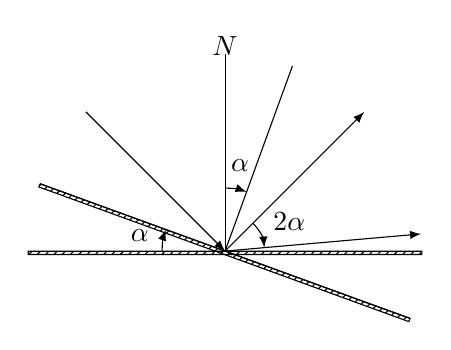
\begin{tikzpicture}
		\draw[-latex] (0:0) -- (5:2.5);
		\draw[latex-] (0:0) -- (135:2.5);
		\draw[-latex] (0:0) -- (45:2.5);
		\draw[-] (0:0) -- (90:2.5);
		\draw[-] (0:0) -- (70:2.5);
		\draw[-] (180:2.5) -- (0:2.5);
		\draw[-] (160:2.5) -- (-20:2.5);
		\filldraw[pattern=north east lines] (180:2.5) -- (0:2.5) -- (-1:2.5) -- (181:2.5) -- (180:2.5);
		\filldraw[pattern=north east lines] (160:2.5) -- (-20:2.5) -- (-21:2.5) -- (161:2.5) -- (160:2.5);
		\draw[-latex] (-0.8,0) arc (180:160:0.8);
		\draw[-latex] (0,0.8) arc (90:70:0.8);
		\draw[-latex] (0.3535,0.3535) arc (45:5:0.5);
		\node[] at (170:1.1) {$\alpha$};
		\node[] at (80:1.1) {$\alpha$};
		\node[] at (25:0.9) {$2\alpha$};
		\node[] at (90:2.6) {$N$};
		\end{tikzpicture}
		\caption{单平面镜对光的变换}
		\label{fig:one-mirror}
	\end{minipage}
	\quad
	\begin{minipage}[t]{0.48\textwidth}
		\centering
		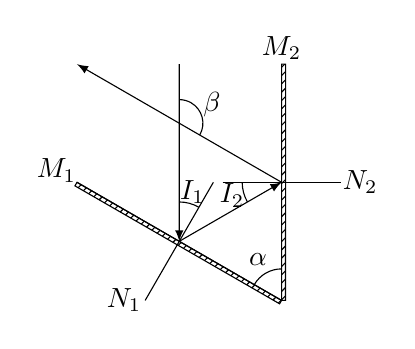
\begin{tikzpicture} 
		\coordinate (A) at (-1.299,3);
		\coordinate (B) at (150:1.5);
		\coordinate (C) at (90:1.5);
		\coordinate (D) at (120:1.732);
		\coordinate (E) at (-0.75,1.5);
		\coordinate (F) at (-1.299,2.25);
		\draw[-] (0:0) -- (90:3);
		\draw[-] (0:0) -- (150:3);
		\filldraw[pattern=north east lines] (0:0) -- (90:3) -- (89:3) -- (0:0.05) -- (0:0);
		\filldraw[pattern=north east lines] (0:0) -- (150:3) -- (151:3) -- (240:0.05) -- (0:0);
		\draw[latex-] (150:1.5) -- (-1.299,3);
		\draw[-latex] (150:1.5) -- (90:1.5);
		\draw[latex-] (-2.598,3) -- (90:1.5);
		\draw[-] (180:1.732) -- (120:1.732);
		\draw[-] (-0.75,1.5) -- (0.75,1.5);
		\node[] at (150:3.3) {$M_1$};
		\node[] at (90:3.2) {$M_2$};
		\node[] at (180:2) {$N_1$};
		\node[] at (1,1.5) {$N_2$};
		\draw[-] (0,0.4) arc (90:150:0.4);
		\node[] at (120:0.6) {$\alpha$};
		\pic["$I_1$", draw=black, -, angle eccentricity=1.3, angle radius=0.5cm] {angle=D--B--A};
		\pic["$I_2$", draw=black, -, angle eccentricity=1.3, angle radius=0.5cm] {angle=E--C--B};
		\pic["$\beta$", draw=black, -, angle eccentricity=1.6, angle radius=0.3cm] {angle=C--F--A};
		\end{tikzpicture}
		\caption{双平面镜对光的变换}
		\label{fig:two-mirror}
	\end{minipage}
\end{figure}

\begin{problem}
	夹角为$35$度的双平面镜系统,当光线以多大的入射角入射于一平面镜时,其反射光线再经另一平面镜反射后,将沿原光路反向射出?
\end{problem}
\begin{solution}
	由\figref{fig:two-mirror} 所示的图像可以看出,若要使光线原路反射,需要垂直入射到第二个平面镜上。根据几何关系可知,入射角为$35$度。
\end{solution}

\begin{problem}
	有一双平面镜系统,光线与其中的一个镜面平行入射,经两次反射后,出射光线与另一镜面平行,问二平面镜的夹角是多少?
\end{problem}
\begin{solution}
	设双平面镜夹角为$\alpha$,由\figref{fig:two-mirror} 所示的图像可以看出,入射光与出射光的夹角为$\alpha$和$2\alpha$,则有$\alpha+2\alpha=180^{\circ}$,得$\alpha=60^{\circ}$。
\end{solution}

\section{平行平板}
\label{sect:parallel-plate}

逐面应用折射球面物像公式(\ref{eq:spherical-refraction}),考虑到$r_1=r_2=\infty$,可得
\begin{equation}
l'=nl,\quad l_2=nl-d,\quad l'=l-\frac{d}{n}
\end{equation}
\begin{equation}
\beta=\beta_1\beta_2=1
\end{equation}
式中$n$和$d$为平行平板的折射率和厚度。

\begin{definition}{平行平板}{parallel-plate}
	由两个相互平行的折射平面构成的光学器件称为平行平板
\end{definition}

\begin{property}
如\figref{fig:parallel-plate-1} 所示,平行平板总对物成同等大小的正立像,物与像总在平板同侧,两者虚实不一致。不论物距为何值,像相对于物的位置总不改变
\end{property}

像相对于物的距离为
\begin{equation}
\Delta l'=-l+d-(-l')=d\bigg(1-\frac{1}{n}\bigg)
\end{equation}
$\Delta l'$恒为正值,所以平行平板所成像总是由物沿光线前进方向沿轴移动$d(1-1/n)$得到,和物的位置、虚实无关。

\begin{figure}[htbp]
	\centering
	\begin{minipage}[t]{0.48\textwidth}
		\centering
		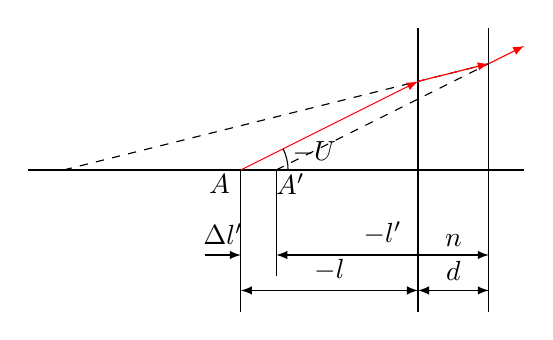
\begin{tikzpicture}[scale=0.9] 
		\draw[-] (-3.5,0) -- (3.5,0);
		\draw[-,name path=pathA] (3,-2) -- (3,2);
		\draw[-,name path=pathB] (2,-2) -- (2,2);
		\draw[-,dashed,name path=pathC] (-3,0) -- (3,1.5);
		\path [name intersections={of = pathB and pathC, by=B}];
		\path [name intersections={of = pathA and pathC, by=C}];
		\draw[-latex,red] (-0.5,0) -- (2,1.25);
		\draw[-,dashed] (0,0) -- (3,1.5);
		\draw[-latex,red] (B) -- (C);
		\draw[-latex,red] (3,1.5) -- (3.5,1.75);
		\node[] at (-0.8,-0.2) {$A$};
		\node[] at (0.2,-0.2) {$A'$};
		\node[] at (2.5,-1) {$n$};
		\coordinate (A) at (0,0);
		\coordinate (D) at (-0.5,0);
		\pic["$-U$", draw=black, -, angle eccentricity=1.6, angle radius=0.6cm] {angle=A--D--B};
		\draw[-] (-0.5,0) -- (-0.5,-2);
		\draw[-] (0,0) -- (0,-1.5);
		\draw[latex-latex](0,-1.2) -- (3,-1.2) node[black,above,midway](line){$-l'$};
		\draw[-latex](-1,-1.2) -- (-0.5,-1.2);
		\node[] at (-0.75,-0.9) {$\Delta l'$};
		\draw[latex-latex](2,-1.7) -- (3,-1.7) node[black,above,midway](line){$d$};
		\draw[latex-latex](2,-1.7) -- (-0.5,-1.7) node[black,above,midway](line){$-l$};
		\end{tikzpicture}
		\caption{平行平板成像(1)}
		\label{fig:parallel-plate-1}
	\end{minipage}
	\quad
	\begin{minipage}[t]{0.48\textwidth}
		\centering
		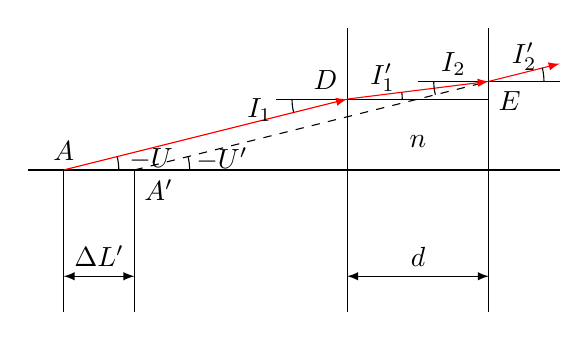
\begin{tikzpicture}[scale=0.9] 
		\draw[-] (-3.5,0) -- (4,0);
		\draw[-] (3,-2) -- (3,2);
		\draw[-] (1,-2) -- (1,2);
		\draw[-] (0,1) -- (3,1);
		\draw[-] (2,1.25) -- (4,1.25);
		\draw[-] (-3,0) -- (-3,-2);
		\draw[-] (-2,0) -- (-2,-2);
		\coordinate [label=above:$A$](A) at (-3,0);
		\coordinate [label=above left:$D$](B) at (1,1);
		\coordinate [label=below right:$A'$](C) at (-2,0);
		\coordinate [label=below right :$E$](D) at (3,1.25);
		\coordinate (E) at (4,1.5);
		\coordinate (F) at (3,0);
		\coordinate (G) at (0,1);
		\coordinate (H) at (3,1);
		\coordinate (I) at (2,1.25);
		\coordinate (J) at (4,1.25);
		\draw[-latex,red] (A) -- (B);
		\draw[-,dashed] (C) -- (D);
		\draw[-latex,red] (B) -- (D);
		\draw[-latex,red] (D) -- (E);
		\pic["$-U$", draw=black, -, angle eccentricity=1.6, angle radius=0.7cm] {angle=C--A--B};
		\pic["$-U'$", draw=black, -, angle eccentricity=1.6, angle radius=0.7cm] {angle=F--C--D};
		\pic["$I_1$", draw=black, -, angle eccentricity=1.6, angle radius=0.7cm] {angle=G--B--A};
		\pic[draw=black, -, angle eccentricity=1.6, angle radius=0.7cm] {angle=H--B--D};
		\node[] at (1.5,1.3) {$I'_1$};
		\pic[draw=black, -, angle eccentricity=1.6, angle radius=0.7cm] {angle=I--D--C};
		\node[] at (2.5,1.5) {$I_2$};
		\pic[draw=black, -, angle eccentricity=1.6, angle radius=0.7cm] {angle=J--D--E};
		\node[] at (3.5,1.6) {$I'_2$};
		\node[] at (2,0.4) {$n$};
		\draw[latex-latex](-3,-1.5) -- (-2,-1.5) node[black,above,midway](line){$\Delta L'$};
		\draw[latex-latex](1,-1.5) -- (3,-1.5) node[black,above,midway](line){$d$};
		\end{tikzpicture}
		\caption{平行平板成像(2)}
		\label{fig:parallel-plate-2}
	\end{minipage}
\end{figure}

\figref{fig:parallel-plate-2} 为非近轴光线经平行平板的折射。产生的位移量为
\begin{equation}
\Delta T'=DE\cdot\sin(I_1-I'_1)=\frac{d}{\cos{I'_1}}\sin(I_1-I'_1)
\end{equation}
可化简为
\begin{equation}
\Delta T'=d\sin I_1\bigg(1-\frac{\cos I_1}{\sqrt{n^2-\sin^2 I_1}}\bigg)
\end{equation}
沿轴方向位移量为
\begin{equation}
\Delta L'=\frac{\Delta T'}{\sin I_1}=d\bigg(1-\frac{\cos I_1}{\sqrt{n^2-\sin^2 I_1}}\bigg)
\end{equation}
或
\begin{equation}
\Delta L'=d\bigg(1-\frac{\tan I'_1}{\tan I_1}\bigg)
\end{equation}
在近轴区,侧向位移量为
\begin{equation}
\Delta t'=d\bigg(1-\frac{1}{n}\bigg)i_1
\end{equation}

\begin{note}
	平行平板不可能以宽光束对物点成完善像,但细光束成像是完善的。近轴区光线的侧向位移量$\Delta t$与入射角$i_1$成线性关系。
\end{note}

\begin{problem}
	有一物镜,其像面与之相距$150\mathrm{mm}$,若在物镜后置一厚度$d=60\mathrm{mm}$,折射率$n=1.5$的平行平板,求
	\begin{enumerate}
		\item 像面位置的变化数值和方向;
		\item 若欲使光轴向上、向下各偏移$5\mathrm{mm}$,平板应正、反转过多大角度?
	\end{enumerate}
\end{problem}
\begin{solution}
	对于第一小问,像面位置变化为$\Delta l'=-l+d-(-l')=d(1-1/n)=60\times(1-1/1.5)=20(\mathrm{mm})$,即向左移动$20\mathrm{mm}$。对于第二小问,由$\Delta t'=d(1-1/n)i_1$,得到$i_1=0.25\mathrm{rad}$,即平板应正、反转过$0.25\mathrm{rad}$角度。
\end{solution}


\section{反射棱镜}
\label{sect:reflecting-prism}

\begin{definition}{反射棱镜}{reflecting-prism}
	由一个或多个反射工作平面磨制在同一块玻璃上的光学零件称为反射棱镜。
\end{definition}

\begin{property}
	奇数次反射成镜像,偶数次反射像不变。
\end{property}

反射棱镜的结构常数为$K$,棱镜通光直径为$D$,棱镜中光轴长度为$d$,有
\begin{equation}
K=\frac{d}{D}
\end{equation}

\begin{problem}
	某棱镜的结构常数为$3.414$,要求通光口径为$10\mathrm{mm}$,求光轴在棱镜中的长度。
	\begin{tasks}(3)
		\task $3.414\mathrm{mm}$
		\task $34.14\mathrm{mm}$
		\task $341.4\mathrm{mm}$
		\task $2.929\mathrm{mm}$
		\task $29.29\mathrm{mm}$
		\task $292.9\mathrm{mm}$
	\end{tasks}
\end{problem}
\begin{solution}
	选择b。
\end{solution}

\subsection{简单棱镜}

\begin{enumerate}
	\item 一次反射棱镜:具有一个反射面,与单个平面镜对应,使物体成镜像。
	\begin{enumerate}
		\item 等腰直角棱镜
		\item 达夫棱镜(如\figref{fig:dove-prism} 所示)
		\begin{figure}[htbp]
			\centering
			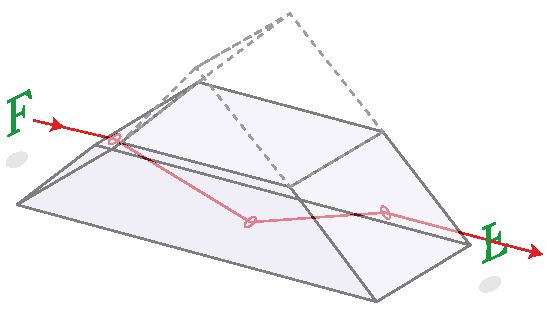
\includegraphics[width=0.5\textwidth]{dove-prism.pdf}
			\caption{达夫棱镜}
			\label{fig:dove-prism}
		\end{figure}
	\end{enumerate}
	\item 二次反射棱镜:有两个反射面,相当于一个双面镜。夹角为$\alpha$的二次反射棱镜使光轴转过$2\alpha$角。
	\begin{enumerate}
		\item 五角棱镜
		\item 半五角棱镜
		\item 二次反射直角棱镜
		\item $30^{\circ}$直角棱镜
		\item 斜方棱镜
	\end{enumerate}
	\item 三次反射棱镜:施密特棱镜,出射光轴相对于入射光轴改变了$45^{\circ}$方向。
\end{enumerate}

\subsection{屋脊棱镜}

\begin{definition}{屋脊棱镜}{roof-prism}
	将普通棱镜的一个反射面用两个互成直角的反射面替代的棱镜即为屋脊棱镜。两直角面的交线为棱线,平行于原反射面,且在主截面上。奇数次反射棱镜,用屋脊面代替其中一个反射面后,就成为了偶数次反射的屋脊棱镜。
\end{definition}

常见的屋脊棱镜有:屋脊直角棱镜、屋脊半五角棱镜、脊棱五角屋镜、屋脊施密特棱镜。

\subsection{角锥棱镜}
角锥棱镜具有三个互成直角的反射面,出射光线方向为入射光线的反方向。

\subsection{棱镜组合}

\begin{figure}[htbp]
	\centering
	\begin{minipage}[t]{0.45\textwidth}
		\centering
		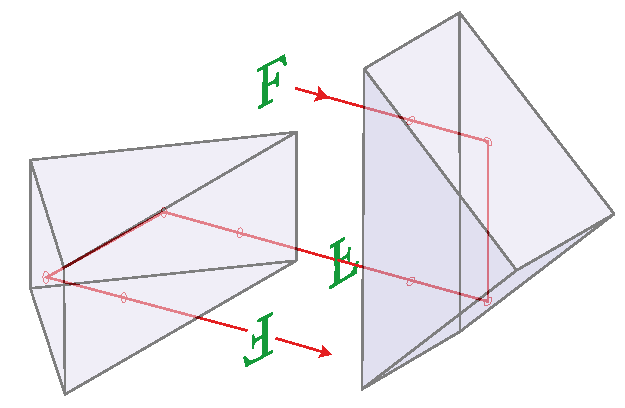
\includegraphics[width=1\textwidth]{double-porro-prism.pdf}
		\caption{普罗棱镜}
		\label{fig:double-porro-prism}
	\end{minipage}
	\qquad
	\begin{minipage}[t]{0.45\textwidth}
		\centering
		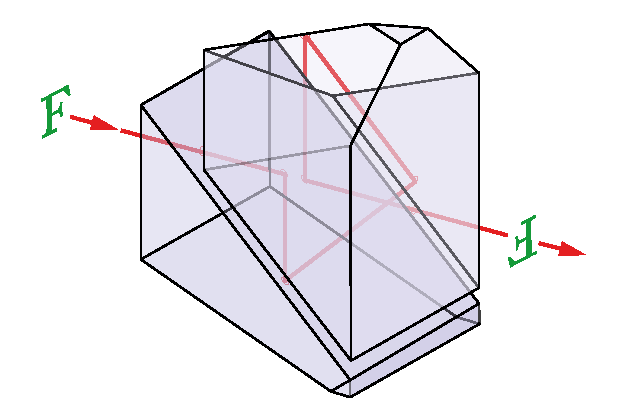
\includegraphics[width=1\textwidth]{schmidt-pechan-prism.pdf}
		\caption{别汉棱镜}
		\label{fig:schmidt-pechan-prism}
	\end{minipage}
\end{figure}

\begin{enumerate}
	\item 普罗棱镜(双普罗棱镜):如\figref{fig:double-porro-prism},由两块相同的等腰直角棱镜组成。
	\item 别汉棱镜(施密特-别汉棱镜组):如\figref{fig:schmidt-pechan-prism},由一块半五角棱镜和一块屋脊施密特棱镜、或一块屋脊半五角棱镜和一块施密特棱镜组成。特点为出射光轴的方向与入射光轴相同,可以让影像做$180^{\circ}$的旋转。
\end{enumerate}

\begin{problem}
	以下棱镜或棱镜组中哪些是成镜像的?
	\begin{tasks}(3)
		\task 别汉棱镜组
		\task 施密特棱镜
		\task 屋脊施密特棱镜
		\task 屋脊五角棱镜
		\task* 一次反射等腰直角棱镜与达夫棱镜的组合
	\end{tasks}
\end{problem}
\begin{solution}
	选择b和d。
\end{solution}

\begin{problem}
	以下光学系统中,可以成镜像的是:
	\begin{tasks}(3)
		\task 平面镜
		\task 别汉棱镜组
		\task 施密特棱镜
		\task 普罗型棱镜组
		\task 屋脊五角棱镜
	\end{tasks}
\end{problem}
\begin{solution}
	选择a、c和e。
\end{solution}

\section{折射棱镜}

\begin{figure}[htbp]
	\centering
	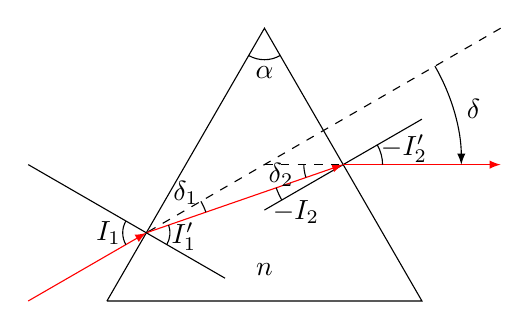
\begin{tikzpicture} 
	\coordinate (A) at (-2,0);
	\coordinate (B) at (0,3.464);
	\coordinate (C) at (2,0);
	\coordinate (D) at (1,1.732);
	\coordinate (E) at (0,1.155);
	\coordinate (F) at (2,2.309);
	\coordinate (G) at (-1.5,0.866);
	\coordinate (H) at (3,3.464);
	\coordinate (I) at (-3,0);
	\coordinate (J) at (-3,1.732);
	\coordinate (K) at (-0.5,0.289);
	\coordinate (L) at (0,1.732);
	\coordinate (M) at (3,1.732);
	\draw[-] (A) -- (B) -- (C) -- (A);
	\draw[-] (E) -- (F);
	\draw[-,dashed] (H) -- (G);
	\draw[-latex,red] (I) -- (G);
	\draw[-latex,red] (G) -- (D);
	\draw[-] (J) -- (K);
	\draw[-,dashed] (L) -- (D);
	\draw[-latex,red] (D) -- (M);
	\pic["$\alpha$", draw=black, -, angle eccentricity=1.4, angle radius=0.4cm] {angle=A--B--C};
	\pic[draw=black, -, angle radius=0.8cm] {angle=D--G--H};
	\pic["$\delta_2$", draw=black, -, angle eccentricity=1.6, angle radius=0.5cm] {angle=L--D--G};
	\pic["$\delta$", draw=black, latex-, angle eccentricity=1.1, angle radius=2.5cm] {angle=M--L--H};
	\pic["$I_1$", draw=black, -, angle eccentricity=1.6, angle radius=0.3cm] {angle=J--G--I};
	\pic["$I'_1$", draw=black, -, angle eccentricity=1.6, angle radius=0.3cm] {angle=K--G--D};
	\pic[draw=black, -, angle radius=0.9cm] {angle=G--D--E};
	\pic["$-I'_2$", draw=black, -, angle eccentricity=1.6, angle radius=0.5cm] {angle=M--D--F};
	\coordinate [label=above:$\delta_1$](delta-1) at (-1,1.1);
	\coordinate [label=below:$-I_2$](i-2) at (0.4,1.4);
	\coordinate [label=above:$n$](n) at (0,0.2);
	\end{tikzpicture}
	\caption{折射棱镜}
	\label{fig:refracting-prism}
\end{figure}

\figref{fig:refracting-prism} 画出了主截面内光线经过棱镜两个折射面折射后的情况。光线偏角为$\delta$,其正负规定为:由入射光线从锐角方向转到出射光线,顺时针为正,反之为负。对两个折射面写出折射定律:
\begin{equation}
\sin I_1=n\sin I'_1,\quad
\sin I'_2=n\sin I_2
\end{equation}
由\figref{fig:refracting-prism} 可得
\begin{equation}
\alpha=I'_1-I_2,\quad\delta=\delta_1+\delta_2=T_1-I'_1+I_2-I'_2
\end{equation}
从而
\begin{equation}
\alpha+\delta=I_1-I'_2
\end{equation}
综合上述公式得到
\begin{equation}
\sin\bigg(\frac{\alpha+\delta}{2}\bigg)=n\sin\frac{\alpha}{2}\cdot\frac{\cos\frac{I'_1+I_2}{2}}{\cos\frac{I_1+I'_2}{2}}
\end{equation}
当$\alpha$和$n$一定时,$\delta$仅随$I_1$而变。最小偏角与$\alpha$和$n$的关系为
\begin{equation}
\sin\bigg(\frac{\alpha+\delta_{\mathrm{min}}}{2}\bigg)=n\sin\frac{\alpha}{2}
\label{eq:minimum-deviation-angle}
\end{equation}

如果折射角很小,偏角公式分为两种情况:
\begin{enumerate}
	\item 光线入射角有一定大小,$I'_1=I_2$,$I_1=I'_2$,有
	\begin{equation}
	\delta=\alpha\bigg(\frac{n\cos I'_1}{\cos I_1}\bigg)
	\end{equation}
	\item 当光线垂直入射或入射角很小,有
	\begin{equation}
	\delta=\alpha(n-1)
	\end{equation}
\end{enumerate}

折射角很小的棱镜称为光楔。当双光楔绕光轴相对旋转,即一个光楔逆时针旋转$\varphi$角,另一个光楔顺时针旋转$\varphi$角,总偏角为$2\varphi$,有
\begin{equation}
\delta=2(n-1)\alpha\cos\frac{\varphi}{2}
\end{equation}

\begin{problem}
	有一等边折射三棱镜,其折射率为$1.65$,求光线经该棱镜的两个折射面折射后产生最小偏角时的入射角,并求出最小偏角值。
\end{problem}
\begin{solution}
	由\figref{fig:refracting-prism} 可知,当$I_1=-I'_2$时,产生最小偏角。由公式$\alpha+\delta=I_1-I'_2$可得,$I_1=55.6^{\circ}$。由式 (\ref{eq:minimum-deviation-angle}) 可得,最小偏角$\delta_m=51.2^{\circ}$。
\end{solution}

\section{光的色散}
以太阳光谱中的夫琅禾费谱线作为特征,单色谱线来表征光学介质的折射率,这些谱线的符号、颜色、波长以及产生谱线的元素如\tabref{tab:spectral-line} 所示。

\begin{table}[htbp]
	\small
	\centering
	\caption{各单色谱线的符号、颜色、波长以及产生谱线的元素}
	\begin{tabular}{c|c|c|c|c|c|c|c|c|c|c}
		\hline
		符号&$A'$&$b$&$C$&$D$&$d$&$e$&$F$&$g$&$G'$&$h$\\
		\hline
		颜色&\multicolumn{3}{c|}{红}&\multicolumn{2}{c|}{黄}&绿&\multicolumn{2}{c|}{青}&蓝&紫\\
		\hline
		$\lambda$(nm)&$768.2$&$706.5$&$656.3$&$589.3$&$587.6$&$546.1$&$486.1$&$435.8$&$434.0$&$404.7$\\
		\hline
		元素&K&He&H&Na&He&Hg&H&Hg&H&Hg\\
		\hline
	\end{tabular}
	\label{tab:spectral-line}
\end{table}

\section{光学材料}
\label{sect:optical-material}
光学玻璃可分为冕牌和火石两大类。冕牌玻璃低折射率低色散,火石玻璃高折射率高色散。阿贝常数$v_D$:
\begin{equation}
v_D=\frac{n_D-1}{n_F-n_C}
\end{equation}

\begin{property}
	阿贝常数越大,色散越低,反之,色散越大。
\end{property}

\begin{problem}
	某种光学玻璃d光的折射率为$1.51637$,$C$光的折射率为$1.51389$,阿贝常数为$64.1$,求$F$光的折射率。
	\begin{tasks}(2)
		\task $1.52196$
		\task $1.50583$
	\end{tasks}
\end{problem}
\begin{solution}
	选择a。
\end{solution}

\begin{problem}
	有一光楔,其材料为K9玻璃($n_F=1.52196$,$n_C=1.51389$),白光经其折射后要发生色散。若要求出射的F光和C光间的夹角$\delta_{F,C}<1'$,求光楔的最大折射角应为多少。
\end{problem}
\begin{solution}
	当光线垂直入射或入射角很小,有$\delta=\alpha(n-1)$。对于F光,出射光线的偏角为$\delta_F=\alpha(n_F-1)$;对于C光,出射光线的偏角为$\delta_C=\alpha(n_C-1)$。其夹角为$\delta_{FC}=\delta_F-\delta_C=\alpha(n_F-1)-\alpha(n_C-1)=0.00807\alpha$。要使$\delta_{FC}=0.00807\alpha<1'$,则有$\alpha=1'/0.00807=2^{\circ}4'4''$。即最大折射角为$2^{\circ}4'4''$。
\end{solution}

\chapter{理想光学系统}

\begin{introduction}
	\item 物像共轭关系(定义 \ref{def:conjugate})
	\item 基点和基面(第 \ref{subsect:base-point} 节)
	\item 光学系统的节点(第 \ref{subsect:nodal-points} 节)
	\item 光学系统的组合(第 \ref{sect:combination-of-optical-systems} 节)
	\item 光焦度(定义 \ref{def:focal-power})
	\item 视觉放大率(定义 \ref{def:visual-magnification})
\end{introduction}

将光学系统在近轴区完善成像的理论推广到任意大的空间,以任意宽的光束都成完善像的光学系统称为理想光学系统。共轴理想光学系统又称为高斯光学。

\section{理想光学系统与共线成像理论}

\begin{definition}{物像共轭关系}{conjugate}
	在理想光学系统中,任何一个物点发出的光线在系统的作用下所有的出射光线仍然相交于一点。由光路的可逆性和折射、反射定律中光线方向的确定性,可得出每一个物点对应于唯一一个像点。通常将这种物像对应关系叫做共轭。
\end{definition}

如果光学系统的物空间和像空间都是均匀透明介质,则入射光线和出射光线均为直线,根据光线的直线传播定律,由符合点对应点的物像空间关系可以推论出直线成像为直线、平面成像为平面的性质。这种点对应点、直线对应直线、平面对应平面的成像变换称为共线成像。

\begin{property}
共轴理想光学系统所成的像的性质:
\begin{enumerate}
	\item 位于光轴上的物点对应的共轭像点必然位于光轴上;位于过光轴的某一个截面内的物点对应的共轭像点必然位于该平面的共轭像面内;同时,过光轴的任意截面成像性质是相同的。
	\item 垂直于光轴平面物所成的共轭平面像的几何形状完全与物相似,在整个物平面上无论哪一部分,物和像的大小比例均等于常数。
	\item 一个共轴理想光学系统,如果已知两对共轭面的位置和放大率,或者一对共轭面的位置和放大率,以及轴上的两对共轭点的位置,则其他一切物点的像点都可以根据这些已知的共轭面和共轭点来表示。
\end{enumerate}
\end{property}

\section{理想光学系统的基点与基面}
\subsection{无限远轴上物点对应的像点}
\label{subsect:infty-object}

\begin{enumerate}	
	\item 无限远轴上物点发出的光线:
	
	设$h$为轴上物点$A$发出的一条入射光线的投射高度,由三角关系近似有
	\begin{equation}
		\tan U=\frac{h}{L}
	\end{equation}
	式中,$U$为孔径角,$L$为物方截距。当$L$趋于无穷大时,物点$A$向无限远处左移,$U$趋于$0$,即无穷远轴上物点发出的光线都与光轴平行。
	\item 像方焦点、焦平面;像方主点、主平面:
	
	如\figref{fig:perfect-optical-system} 所示,平行于光轴的入射光线$AE_1$通过理想光学系统后,出射光线$G'F'$交光轴于$F'$。$F'$为无限远轴上物点的像点,称为像方焦点。过$F'$作垂直于光轴的平面,称为像方焦平面。像方焦平面与无限远处垂直于光轴的物平面共轭。

	\begin{figure}[htbp]
		\centering
		\begin{tikzpicture} 
		\coordinate [label=above left:$O_1$] (A) at (-1,0);
		\coordinate [label=above right:$O_k$] (B) at (1,0);
		\coordinate [label=left:$A$] (C) at (-5,1.3);
		\coordinate [label=right:$A'$] (D) at (5,1.3);
		\coordinate [label=above:$Q'$] (E) at (-0.4,1.8);
		\coordinate [label=above:$Q$] (F) at (0.4,1.8);
		\coordinate [label=above:$F$] (G) at (-4,0);
		\coordinate [label=above:$F'$] (H) at (4,0);
		\coordinate [label=above left:$H'$] (I) at (-0.4,0);
		\coordinate [label=above right:$H$] (J) at (0.4,0);
		\coordinate (K) at (-0.4,1.3);
		\coordinate (L) at (0.4,1.3);
		\coordinate [label=above left:$E_1$] (M) at (-0.8,1.3);
		\coordinate [label=above right:$E_k$] (N) at (0.8,1.3);
		\coordinate [label=above left:$P$] (O) at (-0.8,0.8);
		\coordinate [label=above right:$G'$] (P) at (0.8,0.8);
		\draw[-] (-5,0) -- (5,0);
		\draw[-] (-5,1.3) -- (5,1.3);
		\draw[-] (-4,0) -- (-4,-1);
		\draw[-] (4,0) -- (4,-1.4);
		\draw[-latex] (C) -- (-3,1.3);
		\draw[-latex] (D) -- (3,1.3);
		\draw[-] (-0.4,1.8) -- (-0.4,-1.8);
		\draw[-] (0.4,1.8) -- (0.4,-1.8);
		\draw[latex-] (-4,0) -- (0.4,1.3);
		\draw[latex-] (4,0) -- (-0.4,1.3);
		\draw[line width=0.8pt] (A) arc (180:200:5);
		\draw[line width=0.8pt] (A) arc (180:160:5);
		\draw[line width=0.8pt] (B) arc (180:200:-5);
		\draw[line width=0.8pt] (B) arc (180:160:-5);
		\pic["$-u_1$", draw=black, -, angle eccentricity=1.6, angle radius=0.8cm] {angle=A--G--L};
		\pic["$u'_k$", draw=black, -, angle eccentricity=1.6, angle radius=0.8cm] {angle=K--H--B};
		\draw[latex-latex](-4,-0.8) -- (0.4,-0.8) node[black,below,midway](line){$-f$};
		\draw[latex-latex](4,-1.2) -- (-0.4,-1.2) node[black,below,midway](line){$f'$};
		\draw[latex-latex] (-4.5,1.3) -- ($(A)!(-4.5,1.3)!(B)$)node[black,midway,xshift=0.2cm]{$h_1$};
		\end{tikzpicture}
		\caption{理想光学系统}
		\label{fig:perfect-optical-system}
	\end{figure}
	
	入射光线$AE_1$的延长线与出射光线$G'F'$的反向延长线交于一点$Q'$,过$Q'$作垂直于光轴的平面交光轴于$H'$点,则$H'$点为像方主点,$Q'H'$平面为像方主平面,从主点$H'$搭配焦点$F'$之间的距离为像方焦距$f'$。有
	\begin{equation}
		f'=\frac{h}{\tan U'}
	\end{equation}
	
	\item 无限远轴外物点发出的光线:
	
	进入光学系统的光线总是相互平行的,且与光轴有一定夹角$\omega$。这一束光线经过系统后,一定交于像方焦平面的某一点,这一点为无限远轴外物点的共轭像点。	
\end{enumerate}

\subsection{无限远轴上像点对应的物点}
相关概念同第 \ref{subsect:infty-object} 节内容。物方焦平面上任意一点发出的光线,通过理想光学系统后亦是一组相互平行的光线。

\begin{figure}[htbp]
	\centering
	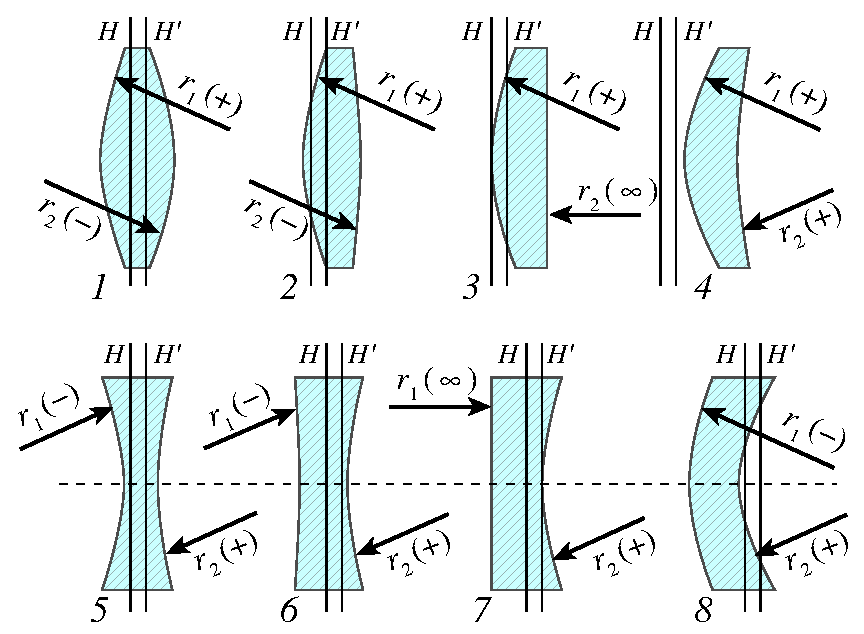
\includegraphics[width=0.6\textwidth]{lens-shapes.pdf}
	\caption{不同形状透镜的主平面}
	\label{fig:lens-shapes}
\end{figure}

\subsection{物方主平面与像方主平面}
\label{subsect:base-point}
如\figref{fig:perfect-optical-system} 所示,两条入射光线$AE_1$和$FP$都经过$Q$,相应地出射光线都经过$Q'$,$Q$和$Q'$为共轭点,因此物方主平面和像方主平面是一对共轭面,垂轴放大率为$+1$。不同形状透镜的主平面位置如\figref{fig:lens-shapes} 所示。对于此类厚透镜的主面位置分析见第 \ref{subsect:thick-lenses} 节。

\begin{definition}{基点和基面}{base-point}
	一对主点和主平面,一对焦点和焦平面,称为共轴理想光学系统的基点和基面。
\end{definition}

\section{理想光学系统的物像关系}
\subsection{牛顿公式}

\begin{figure}[htbp]
	\centering
	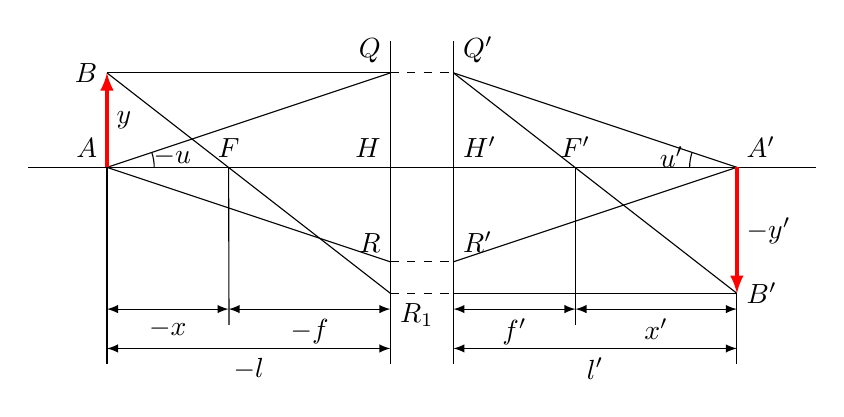
\begin{tikzpicture} 
	\coordinate [label=above left:$Q$] (A) at (-0.4,1.2);
	\coordinate [label=above right:$Q'$] (B) at (0.4,1.2);
	\coordinate [label=above left:$A$] (C) at (-4,0);
	\coordinate [label=above right:$A'$] (D) at (4,0);
	\coordinate [label=above left:$H$] (E) at (-0.4,0);
	\coordinate [label=above right:$H'$] (F) at (0.4,0);
	\coordinate [label=left:$B$] (G) at (-4,1.2);
	\coordinate [label=right:$B'$] (H) at (4,-1.6);
	\coordinate [label=above left:$R$] (I) at (-0.4,-1.2);
	\coordinate [label=above right:$R'$] (J) at (0.4,-1.2);
	\coordinate [label=below right:$R_1$] (K) at (-0.4,-1.6);
	\coordinate [label=above:$F$] (L) at (-2.455,0);
	\coordinate [label=above:$F'$] (M) at (1.95,0);
	\coordinate [label=right:$y$] (N) at (-4,0.6);
	\coordinate [label=right:$-y'$] (O) at (4,-0.8);
	\coordinate (L) at (0.4,-1.6);
	\draw[-] (-5,0) -- (5,0);
	\draw[-] (-0.4,1.6) -- (-0.4,-2.5);
	\draw[-] (0.4,1.6) -- (0.4,-2.5);
	\draw[-] (C) -- (A);
	\draw[-] (D) -- (B);
	\draw[-,dashed] (A) -- (B);
	\draw[-,dashed] (I) -- (J);
	\draw[-,dashed] (K) -- (L);
	\draw[-] (G) -- (A);
	\draw[-] (B) -- (H);
	\draw[-] (C) -- (I);
	\draw[-] (J) -- (D);
	\draw[-] (G) -- (K);
	\draw[-] (L) -- (H);
	\draw[-] (-4,0) -- (-4,-2.5);
	\draw[-] (4,-1.6) -- (4,-2.5);
	\draw[-] (-2.455,0) -- (-2.45,-2);
	\draw[-] (1.95,0) -- (1.95,-2);
	\draw[-latex,red,line width=1.2pt] (C) -- (G);
	\draw[-latex,red,line width=1.2pt] (D) -- (H);
	\draw[latex-latex](-4,-1.8) -- (-2.455,-1.8) node[black,below,midway](line){$-x$};
	\draw[latex-latex](-0.4,-1.8) -- (-2.455,-1.8) node[black,below,midway](line){$-f$};
	\draw[latex-latex](4,-1.8) -- (1.95,-1.8) node[black,below,midway](line){$x'$};
	\draw[latex-latex](0.4,-1.8) -- (1.95,-1.8) node[black,below,midway](line){$f'$};
	\draw[latex-latex](-4,-2.3) -- (-0.4,-2.3) node[black,below,midway](line){$-l$};
	\draw[latex-latex](4,-2.3) -- (0.4,-2.3) node[black,below,midway](line){$l'$};
	\pic["$-u$", draw=black, -, angle eccentricity=1.4, angle radius=0.6cm] {angle=D--C--A};
	\pic["$u'$", draw=black, -, angle eccentricity=1.4, angle radius=0.6cm] {angle=B--D--C};
	\end{tikzpicture}
	\caption{物像位置}
	\label{fig:newton-and-gauss}
\end{figure}

如\figref{fig:newton-and-gauss} 所示,由相似三角形可导出
\begin{equation}
xx'=ff'
\label{eq:newton-eq-1}
\end{equation}
\begin{equation}
\beta=\frac{y'}{y}=-\frac{x'}{f'}=-\frac{f}{x}
\label{eq:newton-eq-2}
\end{equation}
式(\ref{eq:newton-eq-1})为牛顿公式,以焦点为原点。式(\ref{eq:newton-eq-2})为牛顿公式的垂轴放大率公式。

\subsection{高斯公式}
如\figref{fig:newton-and-gauss} 所示,焦物距、焦像距和物距、像距之间有如下关系:
\begin{equation}
x=l-f,\quad x'=l'-f'
\end{equation}
将其带入牛顿公式(\ref{eq:newton-eq-1}),两边同时除以$ll'$可得
\begin{equation}
\frac{f'}{l'}+\frac{f}{l}=1
\label{eq:gauss-eq-1}
\end{equation}
式(\ref{eq:gauss-eq-1})为高斯公式,以主点为原点。其相应的垂轴放大率公式为
\begin{equation}
\beta=\frac{y'}{y}=-\frac{f}{f'}\frac{l'}{l}
\label{eq:gauss-eq-2}
\end{equation}
当物方介质和像方介质相同时,有$f'=-f$,则式(\ref{eq:gauss-eq-1})和式(\ref{eq:gauss-eq-2})可以写成
\begin{equation}
\frac{1}{l'}-\frac{1}{l}=\frac{1}{f'}
\end{equation}
\begin{equation}
\beta=\frac{l'}{l}
\end{equation}

\subsection{两焦距之间的关系}
在近轴光线区域,$fyu=-f'y'u'$,共轴球面系统的近轴区适用拉赫公式$nyu=n'y'u'$,则可得出物方焦距和像方焦距之间的关系式:
\begin{equation}
\frac{f'}{f}=-\frac{n'}{n}
\end{equation}
若光学系统中包括反射面,则两焦距之间的关系由反射面个数决定。设反射面个数为$k$,则有
\begin{equation}
\frac{f'}{f}=(-1)^{k+1}\frac{n'}{n}
\end{equation}
理想光学系统的拉赫公式为
\begin{equation}
ny\tan U=n'y'\tan U'
\label{eq:lah-eq}
\end{equation}

\section{理想光学系统的放大率}
前面已经给出垂轴放大率的公式(\ref{eq:newton-eq-2})和(\ref{eq:gauss-eq-2}),下面给出轴向放大率和角放大率。
\subsection{轴向放大率}
物平面沿光轴移动$\mathrm{d} x$或$\mathrm{d} l$时,像平面移动$\mathrm{d} x'$或$\mathrm{d} l'$,轴向放大率为
\begin{equation}
\alpha=\frac{\mathrm{d} x'}{\mathrm{d} x}=\frac{\mathrm{d} l'}{\mathrm{d} l}
\end{equation}
微分可得
\begin{equation}
\alpha=-\frac{x'}{x}
\end{equation}
将式(\ref{eq:newton-eq-2})带入得
\begin{equation}
\alpha=-\beta^2\frac{f'}{f}=\frac{n'}{n}\beta^2
\end{equation}

\subsection{角放大率}
角放大率为
\begin{equation}
\gamma=\frac{\tan U'}{\tan U}
\end{equation}
根据理想光学系统拉赫公式(\ref{eq:lah-eq})得
\begin{equation}
\gamma=\frac{n}{n'}\frac{1}{\beta}
\end{equation}
理想光学系统三种放大率之间的关系为
\begin{equation}
\alpha\gamma=\beta
\end{equation}

\begin{problem}
	物方、像方介质相同的光学系统对物成像,当$\alpha<1$时,有:
	\begin{tasks}(2)
		\task 物像同向移动,像移动的速度比物快
		\task 物像同向移动,像移动的速度比物慢
		\task 成放大像
		\task 成缩小像
	\end{tasks}
\end{problem}
\begin{solution}
	选择b和d。
\end{solution}

\begin{problem}
	某物方、像方介质相同的折射光学系统对物成像时有$-1<\beta<0$,则当物体向透镜移动时有:
	\begin{tasks}(2)
		\task 像向透镜移动
		\task 像远离透镜移动
		\task 像移动速度比物快
		\task 像移动速度比物慢
	\end{tasks}
\end{problem}
\begin{solution}
	选择b和d。
\end{solution}

\begin{problem}
	无穷远物通过透镜成像放大率为$0$,是否只是一个点?
\end{problem}
\begin{solution}
	并非如此,放大率为$0$只是物在无穷远时公式的计算结果,但实际上并不是一个点。反过来思考:位于焦平面上的物体,成像在无穷远。
\end{solution}

\subsection{光学系统中的节点}
\label{subsect:nodal-points}

\begin{definition}{节点}{nodal-points}
	光学系统中角放大率等于$+1^{\times}$的一对共轭点为节点。厚透镜的节点位置如\figref{fig:nodal-points} 所示
\end{definition}

\begin{property}
	光线通过节点方向不发生改变。
\end{property}

\begin{problem}
	正透镜对虚物成像时:
	\begin{tasks}(4)
		\task 只能成实像
		\task 只能成虚像
		\task 只能成缩小像
		\task 只能成放大像
	\end{tasks}
\end{problem}

\begin{solution}
	选择a和c。
\end{solution}

\begin{problem}
	光学系统的节点是:
	\begin{tasks}(2)
		\task 垂轴放大率为$1$的共轭点
		\task 角放大率为$1$的共轭点
		\task 物方发出过物方节点的光必经过像方节点
		\task 物方发出过像方节点的光必经过物方节点
	\end{tasks}
\end{problem}

\begin{solution}
	选择b和c。
\end{solution}

\begin{figure}[htbp]
	\centering
	\begin{minipage}[t]{0.3\textwidth}
		\centering
		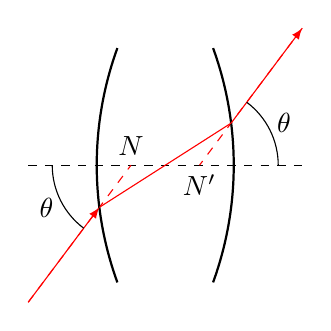
\begin{tikzpicture} [scale=0.87 ] 
		\coordinate (A) at (-1,0);
		\coordinate (B) at (1,0);
		\coordinate [label=above:$N$] (C) at (-0.5,0);
		\coordinate [label=below:$N'$] (D) at (0.5,0);
		\coordinate (E) at (-2,0);
		\coordinate (F) at (2,0);
		\coordinate (G) at (-2,-2);
		\coordinate (H) at (2,2);
		\draw[-,dashed] (E) -- (F);
		\draw[-,dashed,red,name path=pathA] (G) -- (C);
		\draw[-,dashed,red,name path=pathB] (H) -- (D);
		\draw[line width=0.8pt,name path=pathC] (A) arc (180:200:5);
		\draw[line width=0.8pt] (A) arc (180:160:5);
		\draw[line width=0.8pt,name path=pathD] (B) arc (180:200:-5);
		\draw[line width=0.8pt] (B) arc (180:160:-5);
		\path [name intersections={of = pathA and pathC, by=I}];
		\path [name intersections={of = pathB and pathD, by=J}];
		\draw[-,red] (I) -- (J);
		\draw[-latex,red] (G) -- (I);
		\draw[-latex,red] (J) -- (H);
		\pic["$\theta$", draw=black, -, angle eccentricity=1.2, angle radius=1cm] {angle=E--C--G};
		\pic["$\theta$", draw=black, -, angle eccentricity=1.2, angle radius=1cm] {angle=F--D--H};
		\end{tikzpicture}
		\caption{厚透镜的节点}
		\label{fig:nodal-points}
	\end{minipage}
	\quad
	\begin{minipage}[t]{0.6\textwidth}
		\centering
		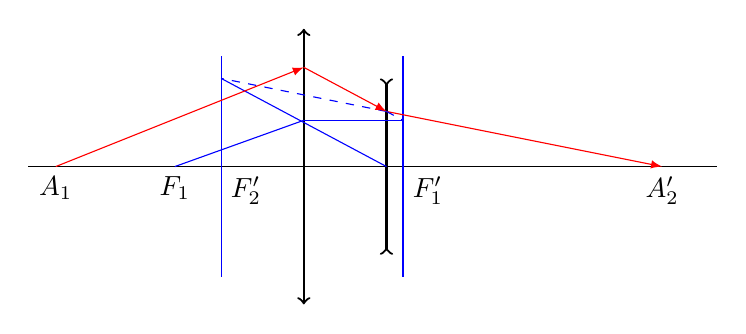
\begin{tikzpicture} [scale=0.7] 
		\draw[-] (-6.5,0) -- (6,0); 
		\draw[<->,line width=0.8pt] (-1.5,2.5) -- (-1.5,-2.5); 
		\draw[>-<,line width=0.8pt] (0,1.6) -- (0,-1.6); 
		\draw[-,blue] (-3,2) -- (-3,-2);
		\draw[-,blue] (0.3,2) -- (0.3,-2);
		\draw[-latex,red] (0,1) -- (5,0);
		\draw[-,dashed,blue] (0,1) -- (-3,1.6);
		\draw[-,dashed,blue] (0,1) -- (0.3,0.84);
		\draw[-,blue] (0,0) -- (-3,1.6);
		\draw[latex-,red] (0,1) -- (-1.5,1.8);
		\draw[-,blue] (0.3,0.84) -- (-1.5,0.84);
		\draw[-,blue] (-3.84,0) -- (-1.5,0.84);
		\draw[-latex,red] (-6,0) -- (-1.5,1.8);
		\coordinate [label=below:$A_1$] (A) at (-6,0);
		\coordinate [label=below:$F_1$] (B) at (-3.84,0);
		\coordinate [label=below right:$F'_2$] (C) at (-3,0);
		\coordinate [label=below right:$F'_1$] (D) at (0.3,0);
		\coordinate [label=below:$A'_2$] (E) at (5,0);
		\end{tikzpicture}
		\caption{图解求像}
		\label{fig:draw-beam-path}
	\end{minipage}
\end{figure}

\section{理想光学系统的图解求像}
画光路图的依据:
\begin{enumerate}
	\item 平行于光轴的光线经理想光学系统后必通过像方焦点;
	\item 过物方焦点的光线经理想光学系统后必为平行于光轴的光线;
	\item 过节点的光线方向不变;
	\item 任意方向的一束平行光经理想光学系统后必交于像方焦平面上一点;
	\item 过物方焦平面上一点的光线经理想光学系统后必为一束平行光;
	\item 主面交点光线高度相同。
\end{enumerate}

\begin{exercise}
	如\figref{fig:draw-beam-path} 所示,已知二光组基点,由物求像或由像求物。
\end{exercise}

\begin{note}
	在这一类绘制光路图的题中,需要注意过第二个透镜光轴处的辅助线与过第一个透镜到其焦面$F_1$的光线平行,这一条线要交于第二个透镜的焦面$F_2$处,经过该交点与光线和第二个透镜的交点的线即为出射光线。图解求像是考试中必考的题目。在大二学习这部分内容的时候,期中考试因为作图题扣了很多分。这一类的题需要多练,如果熟练掌握的话,完全是送分题,否则就是送命题。
\end{note}

\section{理想光学系统的组合}
\label{sect:combination-of-optical-systems}
\begin{figure}[htbp]
	\centering
	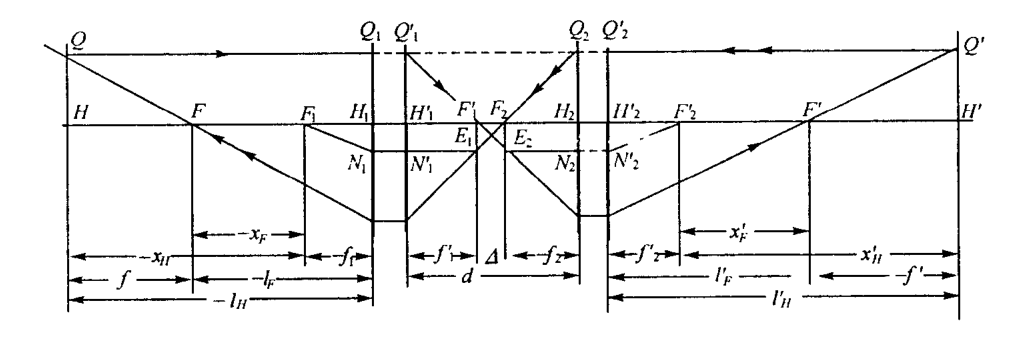
\includegraphics[width=1\textwidth]{combination-of-optical-systems.png}
	\caption{两个光组的组合}
	\label{fig:combination-of-optical-systems}
\end{figure}

\figref{fig:combination-of-optical-systems} 给出了由两个光组组成的等效系统在两个空间的焦点和主点。按牛顿公式,物焦距$x=-\varDelta$,其焦像距$x'_F$为
\begin{equation}
x'_F=-\frac{f_2f'_2}{\varDelta}
\end{equation}
同理有
\begin{equation}
x_F=\frac{f_1f'_1}{\varDelta}
\end{equation}
根据相似三角形$\triangle Q'H'F'$与$\triangle N'_2H'_2F'_2$、$\triangle Q'_1H'_1F'_1$与$\triangle E_2F_2F'_1$,可导出
\begin{equation}
f'=-\frac{f'_1f'_2}{\varDelta}
\label{eq:combination-of-optical-systems-focal-length}
\end{equation}
同理有
\begin{equation}
f=\frac{f_1f_2}{\varDelta}
\end{equation}
大多数情况下光学系统位于空气中,应有$f'_1=-f_1$,$f'_2=-f_2$和$f'=-f$。所以有
\begin{equation}
\varDelta=d-f'_1+f_2=d-f'_1-f'_2
\end{equation}
则有
\begin{equation}
f'=-f=\frac{f'_1f'_2}{f'_1+f'_2-d}
\end{equation}
表示成光焦度形式为
\begin{equation}
\varphi=\varphi_1+\varphi_2-d\varphi_1\varphi_2
\end{equation}

\begin{definition}{折合距离与光焦度}{focal-power}
	一线段的长度除以该线段所在介质的折射率做得的值称为该线段的折合距离。折合焦距的倒数称之为光学系统的光焦度,以$\varPhi$表示,即
	\begin{equation}
	\varPhi=\frac{n'}{f'}=-\frac{n}{f}
	\end{equation}
	如果光学系统位于空气中,其光焦度用$\varphi$表示,即
	\begin{equation}
	\varphi=\frac{1}{f'}=-\frac{1}{f}
	\end{equation}
	光焦度的单位是折光度或屈光度。正光焦度的光学系统对光束起会聚作用;负光焦度的光学系统对光束起发散作用。
\end{definition}

根据\figref{fig:combination-of-optical-systems},还可得到如下关系:
\begin{equation}
\begin{cases}
l'_F=f'_2+x'_F,\quad l_F=f_1+x_F\\
l'_H=l'_F-f',\quad l_H=l_F-f
\end{cases}
\end{equation}
据此可得出等效系统基点相对于主点的位置关系。

等效系统的放大率$\beta$仍可用基本公式$\beta=-f/x$计算。$f$为等效系统的焦距,$x$为物点到等效系统的物方焦点距离,得到
\begin{equation}
\beta=\frac{f_1f_2}{f_1f'_1-x_1\varDelta}
\end{equation}

\begin{problem}
	空气中两光组组合的光焦度公式,如果物方像方或两光组之间的介质不是空气,公式是否会变化,怎么变化,为什么?
\end{problem}
\begin{solution}
	设物方介质折射率为$n_1$,两光组之间折射率为$n_2$,像方折射率为$n_3$。有
	\begin{equation}
	\varDelta=d-f'_1+f_2\notag
	\end{equation}
	\begin{equation}
	f'=\frac{-f'_1f'_2}{\varDelta}\notag
	\end{equation}
	由
	\begin{equation}
	\frac{f'_2}{n_3}=-\frac{f_2}{n_2}\notag
	\end{equation}
	得到
	\begin{equation}
	f'=\frac{f'_1f'_2}{f'_1+\dfrac{n_2}{n_3}f'_2-d}\notag
	\end{equation}
	又有
	\begin{equation}
	\varphi=\frac{n_3}{f'},\quad\varphi_1=\frac{n_2}{f'_1},\quad\varphi_2=\frac{n_3}{f'_2}\notag
	\end{equation}
	所以,光焦度的表达式为
	\begin{equation}
	\varphi=\varphi_2+\varphi_2-\frac{d\varphi_1\varphi_2}{n_2}\notag
	\end{equation}
	由此可知,光焦度与物方像方介质无关,与两光组之间的介质有关。
\end{solution}

\begin{problem}
	一短焦距广角照相物镜的焦距$f'=28\mathrm{mm}$,工作距离$l'_F=40\mathrm{mm}$,总长度(第一透镜到物镜像方焦点的距离)$L=55\mathrm{mm}$,求组成此系统的两个薄透镜的焦距$f'_1$,$f'_2$以及其间隔$d$。
\end{problem}

\begin{problem}
	有一双透镜系统,已知$f'_1=100\mathrm{mm}$,$f'_2=-50\mathrm{mm}$,要求总长度为系统焦距的$0.7$倍,求两透镜的间隔和系统的焦距。
\end{problem}

\begin{problem}
	人眼可简化成一曲率半径为$5.6\mathrm{mm}$的单个折射球面,其像方折射率为$4/3$。求远处对眼睛张角为$1^{\circ}$的物体在视网膜上所成像的大小。
\end{problem}

\section{望远镜系统}

\begin{definition}{望远镜系统}{telescope}
	使入射的平行光束仍保持平行地出射的光学系统称为望远镜系统。望远镜系统的焦距无穷大,焦点和主点位于无穷远。
\end{definition}

\begin{figure}[htbp]
	\centering
	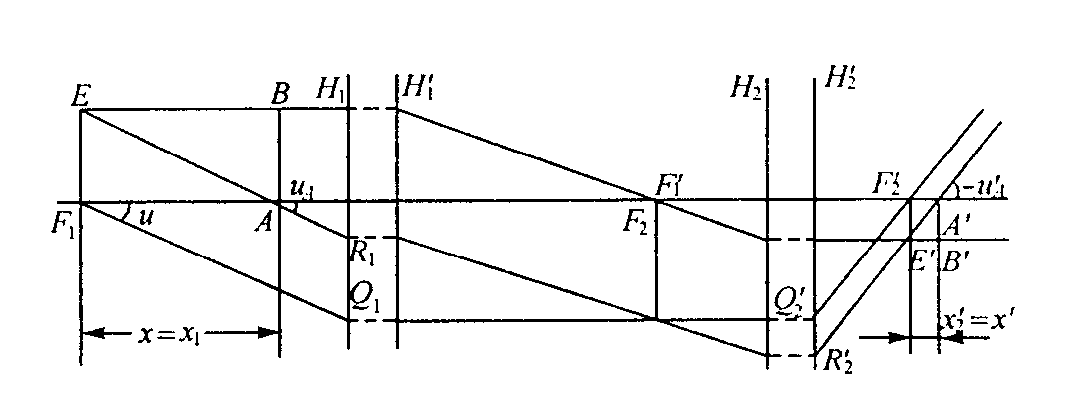
\includegraphics[width=0.7\textwidth]{telescope-system.png}
	\caption{望远镜系统}
	\label{fig:telescope-system}
\end{figure}

如\figref{fig:telescope-system} 所示,根据牛顿公式,并考虑过渡公式$\varDelta=0$,可导出
\begin{equation}
x'_2=\frac{f_2f'_2}{f_1f'_1}x_1
\end{equation}
\begin{equation}
\beta=\beta_1\beta_2=\frac{f_2}{f'_1}
\end{equation}
轴向放大率公式为
\begin{equation}
\alpha=\frac{\mathrm{d}x'_2}{\mathrm{d}x_1}=\frac{f_2f'_2}{f_1f'_1}
\end{equation}
角放大率为
\begin{equation}
\gamma=\frac{\tan u'}{\tan u}=\frac{f_1}{f_2}
\end{equation}
在空气中,$f'_1=-f_1$,$f'_2=-f_2$,因此有
\begin{equation}
\beta=-\frac{f'_2}{f'_1}
\end{equation}
\begin{equation}
\alpha=\beta^2
\end{equation}
\begin{equation}
\gamma=-\frac{f'_1}{f'_2}=\frac{1}{\beta}
\end{equation}
\begin{equation}
x'_2=\alpha x_1
\end{equation}
由此可见,望远镜系统的各种放大率,仅由组成该系统的两个光组的焦距决定。

供眼睛观察用的光学系统为目视光学系统,目视光学系统中最重要的参数为视觉放大率。
\begin{definition}{视觉放大率}{visual-magnification}
	望远镜系统的视觉放大率是远处物体经系统所成的像对眼睛张角$W'$的正切与该物体直接对眼睛张角$W$的正切之比,用$\varGamma$表示。望远镜系统的视觉放大率等于该系统的角放大率,即
	\begin{equation}
	\varGamma=\frac{\tan W'}{\tan W}=\gamma=-\frac{f'_1}{f'_2}=\frac{1}{\beta}
	\end{equation}
	所以,望远镜系统的视觉放大率是物镜焦距与目镜焦距之比。
\end{definition}

一个有限焦距系统之前加角放大率为$\varGamma$的望远镜系统时,整个系统的焦距为原焦距的$\varGamma$倍,即
\begin{equation}
f'=\varGamma f'_2
\end{equation}

\begin{problem}
	开普勒望远镜系统,物方视场增大到一定程度就看不到像了,为什么在物镜和目镜之间加个透镜又能看到像了?这个透镜应该加在何处?
\end{problem}
\begin{solution}
	物方视场增大到一定程度后,折射角仍然过大,光线被拦,所以无法成像。在中间加个透镜,光束会聚,使原本被拦的光线通过,因此可以重新看到像。该透镜为场镜,加在中间的实像面上。
\end{solution}

\begin{problem}
	当物镜焦距大于目镜焦距时,望远镜成放大像还是缩小像?眼睛看到的是放大像还是缩小像?为什么?
\end{problem}
\begin{solution}
	由$\beta=-f'_2/f'_1$可知,$|\beta|<1$,望远镜成缩小像,而$\gamma=1/\beta$,$|\gamma|>1$,视觉放大率大于$1$,眼睛看到的是放大像。
\end{solution}

\begin{problem}
	某望远镜物镜由正、负分离的两个薄透镜组组成,已知$f'_1=500\mathrm{mm}$,$f'_2=-400\mathrm{mm}$,$d=300\mathrm{mm}$,求其焦距。若用此望远镜来观察前方$200\mathrm{mm}$处的物体时,仅用第二个负透镜组来调焦以使其像仍位于物镜的原始焦平面上,问该镜组应向什么方向移动多少距离?此时物镜的焦距为多少?
\end{problem}

\begin{problem}
	\begin{figure}[htbp]
		\centering
		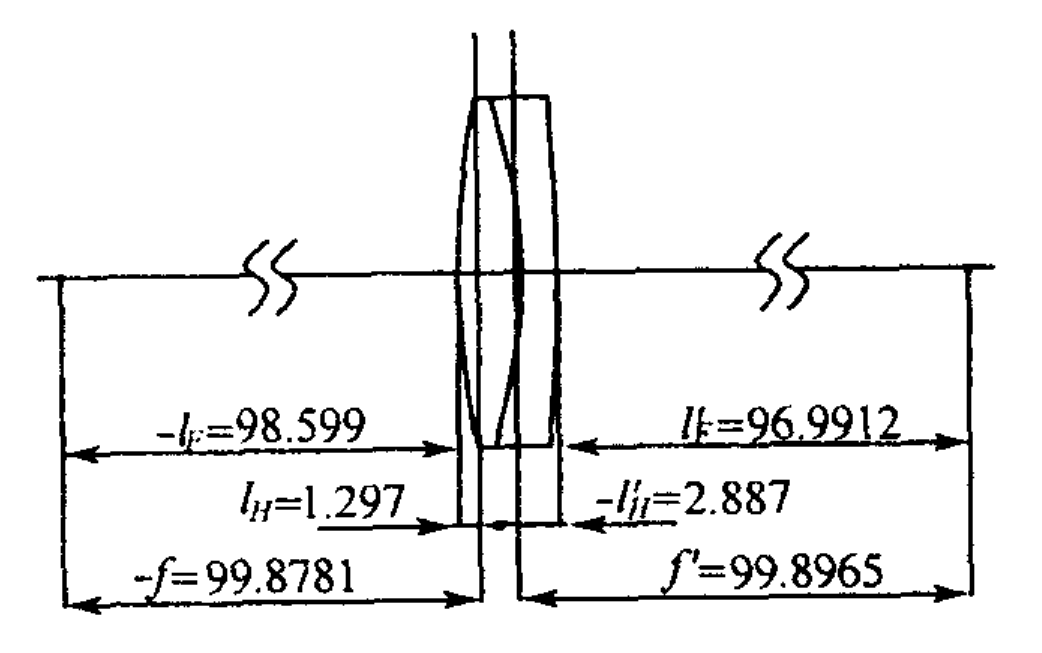
\includegraphics[width=0.5\textwidth]{telescope-objective.png}
		\caption{双胶合望远镜物镜}
		\label{fig:telescope-objective}
	\end{figure}
	如\figref{fig:telescope-objective} 所示的双胶合望远镜物镜,按如下要求分别计算组合系统的焦距和像方基点的位置。
	\begin{enumerate}[(1)]
		\item 在双胶合物镜前加一视觉放大率$\Gamma=-8$的望远镜系统;
		\item 在双胶合物镜前加一视觉放大率$\Gamma=3$的望远镜系统;
		\item 在双胶合物镜后加一厚度为$60\mathrm{mm}$,折射率为$1.5$的平行平板。
	\end{enumerate}
\end{problem}

\section{透镜}
\subsection{薄透镜}

\begin{definition}{薄透镜}{thin-lens}
	透镜的厚度与球面半径相比很小,略去厚度不会引起成像结果的实质性变化,却能对初始阶段的分析和计算带来方便,导出简单的公式。这时认为透镜的厚度为零,称薄透镜。
\end{definition}

薄透镜的物像位置公式:
\begin{equation}
\frac{1}{l'}-\frac{1}{l}=(n-1)\bigg(\frac{1}{r_1}-\frac{1}{r_2}\bigg)
\label{eq:thin-lens}
\end{equation}
焦距为
\begin{equation}
f'=\frac{1}{(n-1)\bigg(\dfrac{1}{r_1}-\dfrac{1}{r_2}\bigg)}
\end{equation}
并有$f=-f'$。其光焦度为
\begin{equation}
\varphi=\frac{1}{f'}=(n-1)\bigg(\frac{1}{r_1}-\frac{1}{r_2}\bigg)
\end{equation}
则式(\ref{eq:thin-lens})可以写成
\begin{equation}
\frac{1}{l'}-\frac{1}{l}=\frac{1}{f'}=\varphi
\end{equation}

由此可知,凸透镜焦距为正,光焦度为正,对光束起会聚作用,像方焦点是对入射平行光束会聚而成的实焦点。凹透镜焦距为负,光焦度为负,对光束起发散作用,像方焦点为虚焦点。因此称凸透镜为正透镜或会聚透镜,凹透镜为负透镜或发散透镜。

通过
\begin{equation}
\beta=\frac{f'}{l+f'}
\end{equation}
可以得出,当$\beta=1$时,解得$l=0$,此时一对物像点重合于薄透镜的中心或顶点,角放大率为$1$,表示这一对共轭点共轭光线有相同方向。因这对共轭点重合于薄透镜中心,所以过薄透镜中心的光线方向不变。

\begin{property}
	薄透镜具有下列性质:
\begin{enumerate}
	\item 平行于光轴入射的光线经透镜后通过像方焦点;
	\item 过物方焦点的入射光线经过透镜后平行于光轴射出;
	\item 通过透镜中心的光线方向不变。
\end{enumerate}
\end{property}

\begin{problem}
	一个$f'=80\mathrm{mm}$的薄透镜当物体位于其前何处时,正好能在透镜前$250\mathrm{mm}$处成像?
	\begin{tasks}(2)
		\task 位于其前$60.6\mathrm{mm}$
		\task 位于其前$117.6\mathrm{mm}$
		\task 位于其后$60.6\mathrm{mm}$
		\task 位于其后$117.6\mathrm{mm}$
	\end{tasks}
\end{problem}
\begin{solution}
	选择a。
\end{solution}

\begin{problem}
	以下光学系统中,对实物一定成虚像的是:
	\begin{tasks}(4)
		\task 反射球面
		\task 平行平板
		\task 负薄透镜
		\task 正薄透镜
	\end{tasks}
\end{problem}
\begin{solution}
	选择b和c。
\end{solution}

\begin{problem}
	单薄透镜成像时,若共轭距(物与像之间的距离)为$250\mathrm{mm}$,求下列情况下透镜应有的焦距:(1) 实物,$\beta=-4$;(2) 实物,$\beta=-1/4$;(3) 虚物,$\beta=-4$;(4) 实物,$\beta=4$;(5) 虚物,$\beta=4$。
\end{problem}
\begin{solution}
	薄透镜的物像位置关系公式为
	\begin{equation}
	\frac{1}{l'}-\frac{1}{l}=\frac{1}{f'}, \quad \beta=\frac{l'}{l} \nonumber
	\end{equation}
	共轭距为
	\begin{equation}
	l'-l=250\mathrm{mm} \nonumber
	\end{equation}
	所以
	\begin{enumerate}[(1)]
		\item 实物,$\beta=-4$。$l'=200\mathrm{mm}$,$l=-50\mathrm{mm}$,$f'=40\mathrm{mm}$。
		\item 实物,$\beta=-1/4$。$l'=50\mathrm{mm}$,$l=-200\mathrm{mm}$,$f'=40\mathrm{mm}$。
		\item 虚物,$\beta=-4$。$l'=-200\mathrm{mm}$,$l=50\mathrm{mm}$,$f'=-40\mathrm{mm}$。
		\item 实物,$\beta=4$。$l'=-1000/3\mathrm{mm}$,$l=-250/3\mathrm{mm}$,$f'=111.11\mathrm{mm}$。
		\item 虚物,$\beta=4$。$l'=1000/3\mathrm{mm}$,$l=250/3\mathrm{mm}$,$f'=-111.11\mathrm{mm}$。
	\end{enumerate}
\end{solution}

\begin{problem}
	用135照相机(物镜的焦距为$50\mathrm{mm}$)拍照时,若要求对身高为$1.7\mathrm{mm}$的人在底片上获得$17\mathrm{mm}$高的像,物镜相对于焦平面的调焦量应为多少?人大致离照相机多少距离?
\end{problem}
\begin{solution}
	由牛顿公式
	\begin{equation}
	\beta=\frac{y'}{y}=-\frac{x'}{f'} \Rightarrow \frac{-17}{1700}=-\frac{x'}{50}\nonumber
	\end{equation}
	得$x'=0.5\mathrm{mm}$;由
	\begin{equation}
	\frac{1}{l'}-\frac{1}{l}=\frac{1}{f'}, \quad \beta=\frac{l'}{l}=-\frac{17}{1700}=-\frac{1}{100} \nonumber
	\end{equation}
	得$l=-5050\mathrm{mm}$。	
\end{solution}

\begin{problem}
	一个焦距为$540\mathrm{mm}$的正薄透镜在其焦平面上给出无穷远物体的像。现欲在透镜之后再插入$f'=200\mathrm{mm}$的薄透镜以使原来的像缩小一半,求此薄透镜的位置。
\end{problem}


\subsection{厚透镜}
\label{subsect:thick-lenses}

如果把透镜的两个球面看作是两个组元,由于已知其焦距和主点的位置,应用组合公式即可求出透镜的焦距和基点位置。

对于单个折射球面,两个主面皆重合于球面的顶点,其焦距可以按照式(\ref{eq:spherical-image-focal-length})和式(\ref{eq:spherical-object-focal-length})写出,即
\begin{equation}
f'=\frac{n'}{n'-n}r \nonumber
\end{equation}
\begin{equation}
f=-\frac{n}{n'-n}r \nonumber
\end{equation}
考虑到透镜在空气中,有$n_1=n'_2=1$,$n'1=n_2=n$,且透镜的光学间隔为$\varDelta=d-f'_1+f_2$,即可通过式(\ref{eq:combination-of-optical-systems-focal-length})得出透镜的焦距公式:
\begin{equation}
f'=-f=\frac{nr_1r_2}{(n-1)[n(r_2-r_1)+(n-1)d]}
\end{equation}
表示成光焦度的形式有
\begin{equation}
\varphi=\frac{1}{f'}=(n-1)(\rho_1-\rho_2)+\frac{(n-1)^2}{n}d\rho_1\rho_2
\end{equation}
其中,$\rho$为球面曲率。还可推出透镜主面位置的公式为
\begin{equation}
l'_H=\frac{-dr_2}{n(r_2-r_1)+(n-1)d},\quad l_H=\frac{-dr_1}{n(r_2-r_1)+(n-1)d}
\end{equation}

对于几种常见的厚透镜(如\figref{fig:thick-lenses})的讨论:
\begin{figure}[htbp]
	\centering
	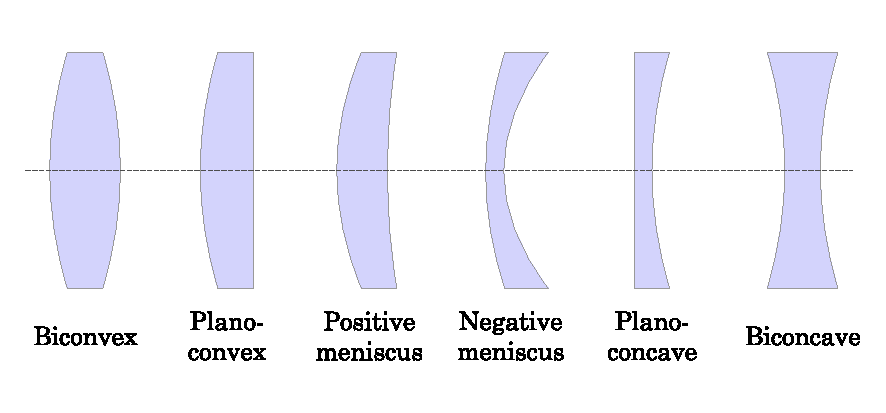
\includegraphics[width=0.8\textwidth]{thick-lenses.pdf}
	\caption{六种常见的厚透镜}
	\label{fig:thick-lenses}
\end{figure}
\begin{enumerate}
	\item 双凸透镜:保持两面的半径不变,随着厚度$d$的不同,其焦距可正可负。当$d<|n(r_2-r_2)/(n-1)|=M$时,$f'$为正,光线会聚,两个主面总位于透镜内部;当$d=M$时,$f'=\infty$;当$d>M$时,$f'$为负,主面在透镜外。
	\item 双凹透镜:$f'$恒为负,发散透镜,两主面位于透镜内部。
	\item 平凸透镜:$f'$恒为正,其值与透镜厚度无关,两主面上的一个相切于球面的顶点,另一个位于透镜内部。
	\item 平凹透镜:$f'$恒为负,其值与透镜厚度无关,两主面上的一个相切于球面的顶点,另一个位于透镜内部。
	\item 弯月形凸透镜:$f'$恒为正,若凸面朝向物方,则物方主面在凸面之前,像方主面在凹面之前,二者都在透镜外。
\end{enumerate}

\section{焦距测量}
焦距的测定有多种方法,这里主要介绍两种。

\textbf{方法一:}用一固定大小的物体经被测透镜或系统在两个位置成像,并量出在这两个共轭位置时的像的大小来计算焦距。如\figref{fig:calculate-focal-length-1} 所示,大小为$y$的物体位于$A_1$时,经被测系统成像于$A'_1$,放大率为$\beta_1$;当物体移动到另一位置$A_2$时,成像于$A'_2$,放大率为$\beta_2$。根据放大率公式$\beta=-f/x$,并令$x_2-x_1=\Delta x$,可导出
\begin{equation}
f=\frac{\Delta x}{\dfrac{1}{\beta_1}-\dfrac{1}{\beta_2}}
\end{equation}
式中,$\Delta x$为物体的移动距离,为已知值,所以只要量出两个位置的像的大小$y'_1$和$y'_2$,即可求知两个$\beta$,并按照上式计算出焦距。

若应用公式$\beta=-x'/f'$,则可得出以像方焦距$f'$表示的相应公式:
\begin{equation}
f'=\frac{\Delta x'}{\beta_1-\beta_2}
\end{equation}
所以,只要量出两个像位置的间距$\Delta x'$和像的大小,即可求得像方焦距。

\begin{figure}[htbp]
	\centering
	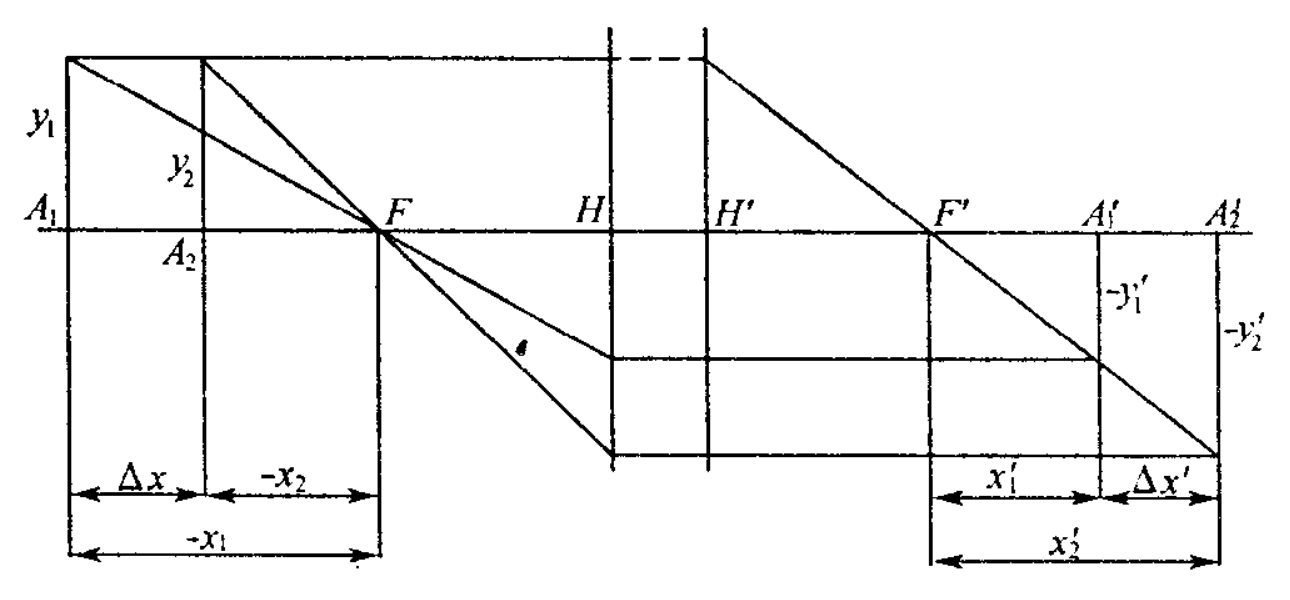
\includegraphics[width=0.4\textwidth]{calculate-focal-length-1.png}
	\caption{焦距测量(一)}
	\label{fig:calculate-focal-length-1}
\end{figure}

\textbf{方法二:}用平行光管测定焦距。如\figref{fig:calculate-focal-length-1} 所示,先看被测系统$O_2$本身的光路。一束与光轴成$W$角的入射平行光束经系统$O_2$以后,会聚于焦平面上的$B'$点。它就是距$O_2$为无限远的某轴外物点的像。$B'$点的高度$y'$可以由一对过节点的共轭光线来确定。通常光学系统位于空气中,主点与节点重合,因此,有图可得
\begin{equation}
y'=-f'\tan U'=-f'\tan W
\end{equation}
这里,给定倾角的平行光束是由平行光管$O_1$提供的,在平行光管$O_1$的前焦面上设置一刻有几对已知间隔线条的分划板,用以产生平行光束。平行光管物镜的焦距经精确测定而为定值,因此与每对刻线对应的平行光束的倾角$\tan W=-y/f_1$也是已知的。所以被测物镜的焦距为
\begin{equation}
f'_2=-\frac{y'}{\tan W}=\frac{f_1}{y}y'
\end{equation}
由此可见,整个测试工作仅在于测得被测物镜焦面上某对刻线的间隔。

\begin{figure}[htbp]
	\centering
	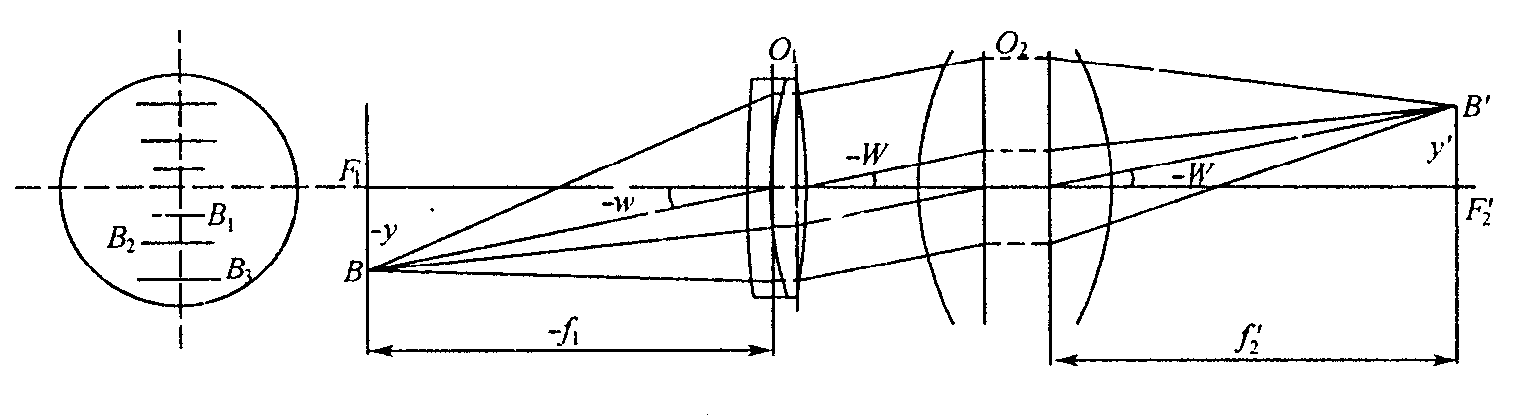
\includegraphics[width=0.7\textwidth]{calculate-focal-length-2.png}
	\caption{焦距测量(二)}
	\label{fig:calculate-focal-length-2}
\end{figure}

\chapter{光学系统中光束的限制}

\begin{introduction}
	\item 孔径光阑(第 \ref{subsect:aperture-stop} 节)
	\item 视场光阑(第 \ref{subsect:field-stop} 节)
	\item 渐晕光阑(第 \ref{subsect:vignetting-stop} 节)
	\item 景深(第 \ref{sect:depth-of-field} 节)
\end{introduction}

\section{光阑}
\subsection{孔径光阑}
\label{subsect:aperture-stop}
\begin{definition}{孔径光阑}{aperture-stop}
在一个光学系统的若干通光孔中,有一个光孔起着限制成像光束(孔径角)的作用。这个光孔就是系统的孔径光阑。严格地说,限制轴上物点孔径角$u$的大小,限制轴上物点成像光束宽度、并有选择轴外物点成像光束位置作用的光阑叫做孔径光阑。
\end{definition}

孔径光阑可以安放在透镜前、透镜上、透镜后,三个位置对\textbf{轴上物点}光束宽度的限制作用是一样的。对于\textbf{轴外物点}参与成像的光束,孔阑位置不同,轴外物点参与成像的光束位置也不同。孔阑位于透镜上时,为使所有轴上物点和轴外物点发出的光束均参与成像所需的透镜口径是最小的。

光瞳是孔径光阑的像。孔径光阑经孔阑前面光学系统所成的像为入射光瞳,经孔阑后面光学系统所成的像为出射光瞳。

孔径光阑、入瞳、出瞳三者互为物像关系。孔阑在系统最前方,系统的入瞳与孔阑重合,孔阑本身就是入瞳;孔阑安放在透镜上,若透镜可当薄透镜处理,则孔阑本身是系统的入瞳和出瞳;孔阑在系统的最后方,系统的出瞳与孔阑重合,孔阑本身为出瞳。

\begin{problem}
	已知照相物镜的焦距为$50\mathrm{mm}$,相对孔径$D/f'=1/4$,入瞳到出瞳的放大率为$\beta_p=1.2$,求出瞳的直径。 
	\begin{tasks}(6)
		\task $12.5\mathrm{mm}$
		\task $200\mathrm{mm}$
		\task $15\mathrm{mm}$
		\task $240\mathrm{mm}$
		\task $10.43\mathrm{mm}$
		\task $166.67\mathrm{mm}$
	\end{tasks}
\end{problem}
\begin{solution}
	选择c。
\end{solution}

\subsection{视场光阑}
\label{subsect:field-stop}
实际光学系统中,物面上发出并进入系统参与成像的光束宽度是有限的,能够清晰成像的物面大小也是有限的。把能够清晰成像的物面范围称为光学系统的物方视场。相应的像面范围为像方视场。

\begin{definition}{视场光阑}{field-stop}
	在物面或像面上安放一个光阑,光阑的大小限定了物面或者像面的大小,即光学系统的成像范围。这个限定成像范围的光阑为视场光阑。
\end{definition}

视场光阑经其前面的光学系统所成的像称为入射窗,经其后面的光学系统所成的像称为出射窗。如果视场光阑安放在物平面上,则入射窗就是视场光阑,出射窗与像平面重合。入射窗、视场光阑、出射窗三者互为物像关系。

\subsection{渐晕光阑}
\label{subsect:vignetting-stop}
\begin{definition}{渐晕光阑}{vignetting-stop}
轴外点和轴上点需要通光全部成像光束的透镜口径大小不一样,轴外点光束部分光被透镜边缘阻挡而不能参与成像,导致轴外点成像光束宽度较轴上点成像光束宽度小,因此像平面边缘比像面中心暗,这种现象就是渐晕,透镜的边缘起拦光作用,为渐晕光阑。
\end{definition}

光孔离孔阑越远,越容易引起渐晕。一般以渐晕系数描述光束渐晕的程度。面渐晕系数是轴外点成像光束在入(出)瞳面上的截面积与入(出)瞳面积之比,线度之比为线渐晕系数。

\begin{figure}[htbp]
	\centering
	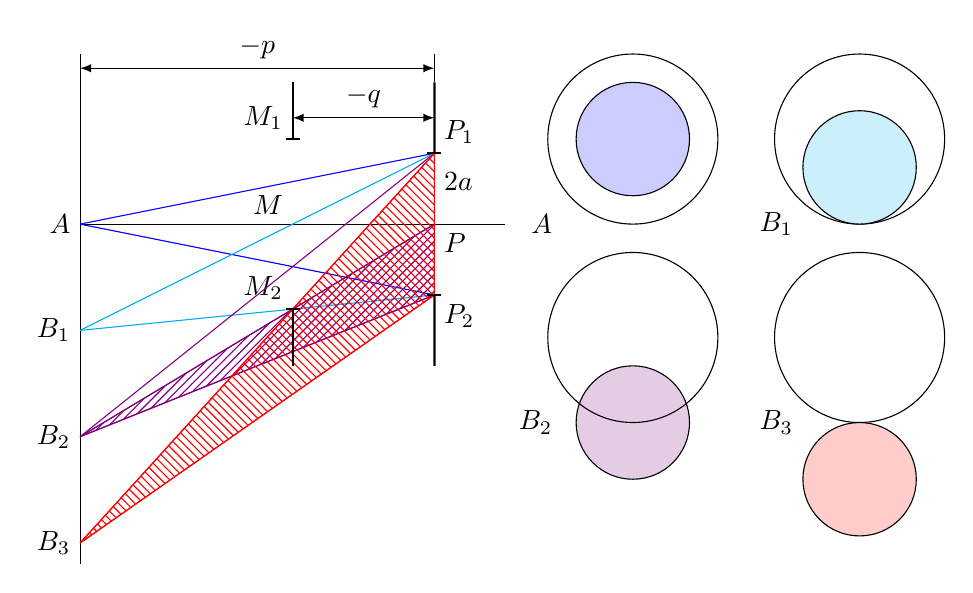
\begin{tikzpicture}[scale=0.9] 
	%\coordinate [label=above left:$P$] (A) at (-1,1);
	\coordinate [label=above right:$P_1$] (A) at (-1,1);
	\coordinate [label=below right:$P_2$] (B) at (-1,-1);
	\coordinate [label=below right:$P$] (C) at (-1,0);
	\coordinate [label=above left:$M_1$] (D) at (-3,1.2);
	\coordinate [label=above left:$M_2$] (E) at (-3,-1.2);
	\coordinate [label=above left:$M$] (F) at (-3,0);
	\coordinate [label=left:$A$] (G) at (-6,0);
	\coordinate [label=left:$B_1$] (H) at (-6,-1.5);
	\coordinate [label=left:$B_2$] (I) at (-6,-3);
	\coordinate [label=left:$B_3$] (J) at (-6,-4.5);
	\coordinate [label=right:$2a$] (K) at (-1,0.6);
	\draw[-] (-6,0) -- (0,0);
	\draw[-] (-6,2.4) -- (-6,-4.8);
	\draw[-,blue] (-6,0) -- (A);
	\draw[-,blue] (-6,0) -- (B);
	\draw[-,cyan] (-6,-1.5) -- (A);
	\draw[-,cyan] (-6,-1.5) -- (B);
	\draw[-,violet] (-6,-3) -- (A);
	\draw[-,violet] (-6,-3) -- (B);
	\draw[-,violet] (-6,-3) -- (C);
	\filldraw[violet,pattern=north east lines,pattern color=violet] (-6,-3) -- (B) -- (C) -- (-6,-3);
	\draw[-,red] (-6,-4.5) -- (A);
	\draw[-,red] (-6,-4.5) -- (B);
	\filldraw[red,pattern=north west lines,pattern color=red] (-6,-4.5) -- (A) -- (B) -- (-6,-4.5);
	\draw[-,line width=0.8pt] (-1,2) -- (A);
	\draw[-,line width=0.8pt] (-0.9,1) -- (-1.1,1);
	\draw[-,line width=0.8pt] (-1,-2) -- (B);
	\draw[-,line width=0.8pt] (-0.9,-1) -- (-1.1,-1);
	\draw[-,line width=0.8pt] (-3,2) -- (-3,1.2);
	\draw[-,line width=0.8pt] (-3.1,1.2) -- (-2.9,1.2);
	\draw[-,line width=0.8pt] (-3,-2) -- (-3,-1.2);
	\draw[-,line width=0.8pt] (-3.1,-1.2) -- (-2.9,-1.2);
	\draw[-] (-1,2.4) -- (-1,2);
	\draw[latex-latex](-3,1.5) -- (-1,1.5) node[black,above,midway](line){$-q$};
	\draw[latex-latex](-6,2.2) -- (-1,2.2) node[black,above,midway](line){$-p$};
	\draw (1.8,1.2) circle (1.2);
	\coordinate [label=left:$A$] (G1) at (0.8,0);
	\filldraw [fill=blue!20] (1.8,1.2) circle (0.8);
	\draw (5,1.2) circle (1.2);
	\coordinate [label=left:$B_1$] (H1) at (4.2,0);
	\filldraw [fill=cyan!20] (5,0.8) circle (0.8);
	\filldraw [fill=violet!20] (1.8,-2.8) circle (0.8);
	\draw (1.8,-1.6) circle (1.2);
	\coordinate [label=left:$B_2$] (I1) at (0.8,-2.8);
	\draw (5,-1.6) circle (1.2);
	\coordinate [label=left:$B_3$] (J1) at (4.2,-2.8);
	\filldraw [fill=red!20] (5,-3.6) circle (0.8);
	\end{tikzpicture}
	\caption{渐晕光阑在物空间的像}
	\label{fig:vignetting-stop}
\end{figure}

\figref{fig:vignetting-stop} 所示的是渐晕光阑在物空间的像。$A$到$B_1$发出的光束都不被遮拦,无渐晕;$B_2$发出的光束主光线以下部分被遮拦,半渐晕;$B_3$发出的光束只有一条光线通过,此处为最大成像范围;$B_3$以下的光束不能成像。由相似三角形关系可得
\begin{equation}
\frac{2a}{B_1B_3}=\frac{-q}{-p+q}
\end{equation}
即
\begin{equation}
B_1B_3=2a\frac{q-p}{q}
\end{equation}
如果$B_1B_3=0$,则无渐晕,即$p=q$。渐晕光阑在物空间的像与物面重合是不产生渐晕的必要条件。

\begin{note}当一个光学系统无视场光阑时:
	\begin{enumerate}
		\item 将所有光孔投射到第一个光孔的物空间,对入瞳中心张角最小的那个光孔像所共轭的光孔称为渐晕光阑。
		\item 将所有光孔投射到最后一个光孔的像空间,对出瞳中心张角最小的那个光孔像所共轭的光孔称为渐晕光阑。
		\item 当孔径光阑无限小时,渐晕光阑直接限制了成像范围,因此过去也称其为视场光阑,称其像为入射窗、出射窗。
		\item 当一个光学系统有视场光阑时,也可能有渐晕光阑,此时渐晕光阑起拦光作用。
	\end{enumerate}
\end{note}

\begin{remark}
	所有系统都有孔径光阑,视场光阑和渐晕光阑二者至少有其一。
\end{remark}

\begin{problem}
	是否所有光学系统都要无渐晕?
\end{problem}
\begin{solution}
	当孔径和视场都较大时,无渐晕,既不必要也不可能。因为远离孔阑的透镜直径不能做得太大,且适当拦掉偏离理想成像状态较远的像差较大的轴外光束有利于改善像质。故常有适当渐晕,一般允许$50\%$,必要时$30\%$。
\end{solution}

\begin{problem}
	渐晕光阑是否只有一个?
\end{problem}
\begin{solution}
	孔阑在光学系统内部时,可能有两个渐晕光阑,一个拦上光线,一个拦下光线。特别是全对称系统,必有两个渐晕光阑。
\end{solution}

\begin{problem}
	成像光可以看成光线路径上任何一点发出的。如果看成孔阑发出的,视阑起什么作用?
\end{problem}
\begin{solution}
	视阑起孔阑的作用。将孔阑看做光源,对入瞳中心张角最小的光阑是原来的视阑。
\end{solution}

\section{景深}
\label{sect:depth-of-field}

\begin{figure}[htbp]
	\centering
	\begin{tikzpicture}[scale=1] 
	%\coordinate [label=above left:$P$] (A) at (-1,1);
	\coordinate [label=above:$P$] (A) at (0.5,0);
	\coordinate [label=above left:$P_1$] (A1) at (0.5,1);
	\coordinate [label=above left:$P_2$] (A2) at (0.5,-1);
	\coordinate [label=above:$P'$] (B) at (1.5,0);
	\coordinate [label=above right:$P'_1$] (B1) at (1.5,1);
	\coordinate [label=above right:$P'_2$] (B2) at (1.5,-1);
	\coordinate [label=above left:$A$] (C) at (-4.2,0);
	\coordinate [label=above left:$B_1$] (C1) at (-6,2.75);
	\coordinate [label=above left:$B_2$] (C2) at (-2.98,-1.5);
	\coordinate [label=above right:$A'$] (D) at (4,0);
	\coordinate [label=below left:$B'_2$] (D1) at (3.42,-1);
	\coordinate [label=above right:$B'_2$] (D2) at (5,2);
	\coordinate [label=above:对准平面] (E) at (-4.2,3);
	\coordinate [label=above left:入射光瞳] (F) at (0.5,2);
	\coordinate [label=above right:出射光瞳] (G) at (1.5,2);
	\coordinate [label=above:景像平面] (H) at (4,3);
	\coordinate [label=above right:$Z_1$] (Z1) at (-4.2,2);
	\coordinate [label=left:$Z_2$] (Z2) at (-4.2,-2);
	\coordinate [label=above left:$Z'_1$] (Z1) at (4,1.2);
	\coordinate [label=right:$Z'_2$] (Z2) at (4,-1.3);
	\draw[-] (-6.5,0) -- (5.5,0);
	\draw[-,line width=0.8pt] (A1) -- (0.5,2);
	\draw[-,line width=0.8pt] (A2) -- (0.5,-2);
	\draw[-,line width=0.8pt] (B1) -- (1.5,2);
	\draw[-,line width=0.8pt] (B2) -- (1.5,-2);
	\draw[-,line width=0.8pt] (-4.2,3) -- (-4.2,-3);
	\draw[-] (-6,3) -- (-6,-4.5);
	\draw[-] (-2.98,3) -- (-2.98,-3.5);
	\draw[-latex] (C) -- (A);
	\draw[-latex] (C) -- (A1);
	\draw[-latex] (C) -- (A2);
	%\draw[-latex] (-4.2,2) -- (A);
	\draw[-latex,red] (C1) -- (A);
	\draw[-latex,red] (C1) -- (A1);
	\draw[-latex,red] (C1) -- (A2);
	%\draw[-latex] (-6,-2.75) -- (A);
	\draw[-latex,blue] (-4.2,-2) -- (A);
	\draw[-latex,blue] (-4.2,-1.65) -- (A2);
	\draw[-latex,blue] (-4.2,-2.35) -- (A1);
	\draw[-,line width=0.8pt] (4,3) -- (4,-3);
	\draw[-] (5,3) -- (5,-4.5);
	\draw[-] (3.42,3) -- (3.42,-3.5);
	\draw[latex-] (D) -- (B1);
	\draw[latex-] (D) -- (B2);
	\draw[latex-,blue] (D2) -- (B);
	\draw[latex-,blue] (D2) -- (B1);
	\draw[latex-,blue] (D2) -- (B2);
	\draw[latex-,red] (4,-1.4) -- (B);
	\draw[latex-,red] (4,-1.7) -- (B1);
	\draw[latex-,red] (4,-1.1) -- (B2);
	\draw[-] (0.5,1) -- (1,1);
	\draw[-] (0.5,-1) -- (1,-1);
	\draw[black,latex-latex](0.75,1) -- (0.75,-1) node[black,below right,midway](line){$2a$};
	\draw[-] (0.5,-2.5) -- (0.5,-4.5);
	\draw[-] (1.5,-2.5) -- (1.5,-4.5);
	\draw[-] (-4.2,-3) -- (-4.2,-4);
	\draw[-] (4,-3) -- (4,-4);
	\draw[black,latex-latex](-6,-3.2) -- (-4.2,-3.2) node[black,above,midway](line){$\varDelta_1$};
	\draw[black,latex-latex](-2.98,-3.2) -- (-4.2,-3.2) node[black,above,midway](line){$\varDelta_2$};
	\draw[black,latex-latex](-2.98,-3.2) -- (0.5,-3.2) node[black,above,midway](line){$-p_2$};
	\draw[black,latex-latex](3.42,-3.2) -- (1.5,-3.2) node[black,above,midway](line){$p'_1$};
	\draw[black,latex-latex](-4.2,-3.7) -- (0.5,-3.7) node[black,above,midway](line){$-p$};
	\draw[black,latex-latex](4,-3.7) -- (1.5,-3.7) node[black,above,midway](line){$p'$};
	\draw[black,latex-latex](-6,-4.2) -- (0.5,-4.2) node[black,above,midway](line){$-p_1$};
	\draw[black,latex-latex](5,-4.2) -- (1.5,-4.2) node[black,above,midway](line){$p'_2$};
	\end{tikzpicture}
	\caption{景深示意图}
	\label{fig:depth-of-field}
\end{figure}

如\figref{fig:depth-of-field} 所示,空间点$B_1$、$B_2$位于景像平面的共轭面(对准平面)以外,所成像为弥散斑,在景像平面上的弥散斑大小与入射光瞳大小、空间点距对准平面的距离有关,如果弥散斑足够小,小于人眼极限分辨角,则人眼认为其为清晰像。能在像平面上获得清晰像的空间深度称为景深。

能在景像平面上成清晰像的最远平面为远景,最近平面为近景。根据三角形相似关系,当已知入瞳直径$2\alpha$以及远景平面、近景平面和对准平面到入瞳的距离$p_1$、$p_2$、$p$时,即可求出远景和近景平面上物点的成像光束在对准平面上的截面大小$Z_1$、$Z_2$。此二截面被系统成像于景象平面上,称为弥散斑,小到一定程度可认为是清晰的像,所以对其有相同的限制。可解得远景和近景平面到入瞳的距离分别为
\begin{equation}
p_1=\frac{2ap}{2a-Z},\quad p_2=\frac{2ap}{2a+Z}
\end{equation}
由于$Z=Z'/\beta$,并将放大率$\beta$近似地写成$\beta=f'/p$,得
\begin{equation}
p_1=\frac{2apf'}{2af'-pZ'},\quad p_2=\frac{2apf'}{2af'+pZ'}
\end{equation}
由此,远景和近景到对准平面的距离分别为
\begin{equation}
\varDelta_1=p_1-p=\frac{p^2Z'}{2af'-pZ'},\quad \varDelta_2=p-p_2=\frac{p^2Z'}{2af'+pZ'}
\end{equation}
$\varDelta_1$和$\varDelta_2$分别为远景深度和近景深度,二者之和为总的成像空间深度,即景深
\begin{equation}
\varDelta=\varDelta_1+\varDelta_2=\frac{4af'p^2Z'}{4a^2f'^2-p^2Z'^2}
\end{equation}
当景象平面弥散斑大小规定后,景深与系统的入射直径、焦距和对准平面的距离有关。入瞳直径越大,焦距越大,景深越小;拍摄距离越大,景深越大;远景深度$\varDelta_1$总要比近景深度$\varDelta_2$大。

\begin{problem}
	要得到远近都清楚的照片,应选用: 
	\begin{tasks}(2)
		\task 大孔径短焦距
		\task 小孔径长焦距
		\task 小孔径短焦距
		\task 长对准距离长焦距
	\end{tasks}
\end{problem}
\begin{solution}
	选择c。
\end{solution}

\section{远心光学系统}
远心光学系统的孔阑设于焦平面上,其中,物方远心光路的孔阑与$F'$重合,入瞳位于物方无穷远,物方主光线平行于光轴;像方远心光路的孔阑与$F$重合,出瞳位于像方无穷远,像方主光线平行于光轴。\figref{fig:telecentric-optical-system} 所示的是一种物方远心光学系统(光从右侧入射)。

\begin{figure}[htbp]
	\centering
	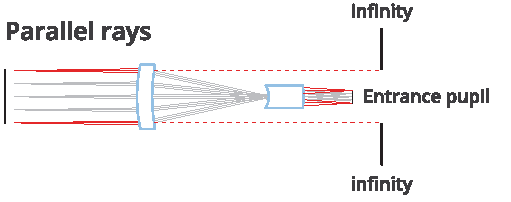
\includegraphics[width=0.6\textwidth]{telecentric-optical-system.pdf}
	\caption{物方远心光学系统}
	\label{fig:telecentric-optical-system}
\end{figure}

\chapter{光能及其计算}

\begin{introduction}
	\item 辐射能通量(定义 \ref{def:radiant-flux})
	\item 光通量(定义 \ref{def:luminous-flux})
	\item 发光强度(定义 \ref{def:luminous-intensity})
	\item 光照度(定义 \ref{def:illuminance})
	\item 光出射度(定义 \ref{def:luminous-exitance})
	\item 光亮度(定义 \ref{def:brightness})
\end{introduction}

\section{辐射能通量与光通量}

\begin{definition}{辐射能通量}{radiant-flux}
	某一瞬间通过某一面积的全部辐射能与通过时间的 比值称为辐射能通量,单位为瓦,即
	\begin{equation}
	W=\frac{\mathrm{d}E}{\mathrm{d}t}(\mathrm{W})
	\end{equation}
\end{definition}

设$P_\lambda$是某一波长附近单位波长间隔内所具有的功率,称辐射能通量随波长的分布函数,则在某一微小波长范围$\mathrm{d}\lambda$内所包含的辐射能通量为
\begin{equation}
\mathrm{d}W_{\lambda,\lambda+\mathrm{d}\lambda}=P_{\lambda}\cdot\mathrm{d}\lambda
\end{equation}
辐射体的总辐射能通量为
\begin{equation}
W=\int_{\lambda} P_{\lambda}\cdot\mathrm{d}\lambda
\end{equation}
人眼对于波长为$555\mathrm{nm}$的光最为敏感,如果在单位波长内$P_{\lambda}\mathrm{W}$的辐射能通量相当于$\varPhi_{\lambda}$流明的光通量,其比值为
\begin{equation}
K_{\lambda}=\frac{\varPhi_{\lambda}}{P_{\lambda}}
\end{equation}
可表示为$1\mathrm{W}$单色辐射能通量所相当的流明数。$555\mathrm{nm}$光的这一数值$K_{555}$为最大。任意其他波长的单色光的$K_{\lambda}$值与$K_{555}$之比表征了人眼对于该单色辐射的灵敏度,称为光谱光视效率或视见函数,以$V_{\lambda}$表示,即
\begin{equation}
V_{\lambda}=\frac{K_{\lambda}}{K_{555}}
\end{equation}
在极小的波长间隔内,有
\begin{equation}
\mathrm{d}\varPhi=V_{\lambda}P_{\lambda}\cdot\mathrm{d}\lambda
\end{equation}
则总光通量为
\begin{equation}
\varPhi=\int_{\lambda}V_{\lambda}P_{\lambda}\cdot\mathrm{d}\lambda
\end{equation}
此式给出的光通量单位为瓦,若将其表示成流明,应有
\begin{equation}
\varPhi=K_{555}\int_{\lambda}V_{\lambda}P_{\lambda}\cdot\mathrm{d}\lambda
\end{equation}
一个辐射体或光源发出的总光通量与总辐射能通量之比$\eta$称为光源的发光效率,即
\begin{equation}
\eta=\frac{\varPhi}{W}
\end{equation}
其表示为每瓦辐射能通量所产生的的光通量。

\section{五种光学量的含义}

\subsection{光通量}
\begin{definition}{光通量}{luminous-flux}
标度可见光对人眼的视觉刺激程度的量。单位为流明($\mathrm{lm}$)。
\end{definition}
上一节已详细说明其具体内容。

\subsection{发光强度}
\begin{definition}{发光强度}{luminous-intensity}
点光源向各个方向发出光能,在某一方向上,立体角$\mathrm{d}\omega$内发出的光通量$\mathrm{d}\varPhi$与该立体角的比值为点光源在该方向上的发光强度,即
\begin{equation}
I=\frac{\mathrm{d}\varPhi}{\mathrm{d}\omega}
\end{equation}
对于均匀发光的光源,其$I=I_0$为常数,此时有
\begin{equation}
I_0=\frac{\varPhi}{\omega}
\end{equation}
发光强度的单位是坎德拉($\mathrm{cd}$)。
\end{definition}
点光源周围空间的总立体角为$4\pi$,所以这种点光源向四周发出的总光通量为
\begin{equation}
\varPhi=4\pi I_0
\end{equation}
对于发光强度随方向变化的光源,其在各个方向的光通量不相同,因此$\varPhi/4\pi$仅为平均发光强度。将位于原点的点光源在由$i$和$\varphi$角所决定的方向上的发光强度表示为$I(\varphi,i)$,立体角的微分表达式为
\begin{equation}
\mathrm{d}\omega=\sin i\cdot\mathrm{d}i\cdot\mathrm{d}\varphi
\end{equation}
则对$\mathrm{d}\varPhi$在整个空间积分即可求出总光通量,有
\begin{equation}
1\mathrm{lm}=1\mathrm{cd}\cdot\mathrm{sr}
\end{equation}
\begin{note}
	实际中常常需要求出各项均匀发光的点光源在锥角为$\alpha$的锥体内发出的光通量,若锥体与$y$轴重合,且点光源位于光学系统的光轴上,则其对于入瞳张角为$2U$的光通量为
	\begin{equation}
	\varPhi=4\pi I_0\sin^2\frac{U}{2}
	\end{equation}
\end{note}

\subsection{光照度}
\begin{definition}{光照度}{illuminance}
在某一微小面积$\mathrm{d}S$上投射的光通量$\mathrm{d}\varPhi$与该面积的比值$E$称为该面积上的光照度,即
\begin{equation}
E=\frac{\mathrm{d}\varPhi}{\mathrm{d}S}
\end{equation}
如果光通量是均匀射入受照表面的,则有
\begin{equation}
E=\frac{\varPhi}{S}
\end{equation}
光照度的单位是勒克斯($\mathrm{lx}$),有
\begin{equation}
1\mathrm{lx}=1\mathrm{lm/m^2}=1\mathrm{cd\cdot sr/m^2}
\end{equation}
\end{definition}
\begin{note}
	发光强度为$I$的点光源$C$照明相距$R$处的面积为$\mathrm{d}S$时,该面积对点光源所张的立体角是
	\begin{equation}
	\mathrm{d}\omega=\frac{\mathrm{d}S_n}{R^2}=\frac{\mathrm{d}S\cdot\cos i}{R^2}
	\end{equation}
	点光源在此立体角内发出的光通量为$\mathrm{d}\varPhi=I\mathrm{d}\omega$,得$\mathrm{d}S$上的光照度为
	\begin{equation}
	E=\frac{I\cdot\cos i}{R^2}
	\end{equation}
	由此可见,由点光源直接照射到某一面积所产生的的光照度与光源的发光强度成正比,与受照面积的距离平方成反比,且与照射方向有关,垂直照射时光照度最大。
\end{note}

\begin{problem}
	一房间为$4.8\times6.4$平方米,中间安装了一个发光强度为$200$坎德拉的均匀发光灯泡,灯离地板的高度为$3$米,求房间角落地面上的照度。  
	\begin{tasks}(5)
		\task $6.4$勒克斯
		\task $4.8$勒克斯
		\task $3.6$勒克斯
		\task $0.96$勒克斯
		\task $2.89$勒克斯
	\end{tasks}
\end{problem}
\begin{solution}
	选择b。
\end{solution}

\subsection{光出射度}
\begin{definition}{光出射度}{luminous-exitance}
某一发光表面上微小面积范围内所发出的光通量与该面积之比称为该面积上的光出射度,即
\begin{equation}
M=\frac{\mathrm{d}\varPhi}{\mathrm{d}S}
\end{equation}
若为均匀发光表面,且在$2\pi$立体角内发出的光通量为$\varPhi$,则
\begin{equation}
M=\frac{\varPhi}{S}
\end{equation}
\end{definition}
光出射度与光照度的形式相同,其差别在于光照度中的$\varPhi$是表面接收的光通量,光出射度中的$\varPhi$是从表面发出的光通量。光出射度的单位为勒克斯($\mathrm{lx}$)。二次光源的光出射度与受照后的光照度和表面的反射率有关,可表示为
\begin{equation}
M=\rho E
\label{eq:luminous-exitance}
\end{equation}

\subsection{光亮度}
\begin{definition}{光亮度}{brightness}
	在光源表面划出一元面积$\mathrm{d}S$,在与法线$N$成$i$角的方向上,由元面积$\mathrm{d}S$和受照小面积所限定的范围内,从该元面积所发出的光通量应与立体角$\mathrm{d}\omega$和元面积在垂直于光束轴线的平面上的投影$\mathrm{d}S_n$成正比,用$L_i$表示比例系数,则称此比例系数为光源在与法线成$i$角方向上的光亮度。即
	\begin{equation}
	\mathrm{d}\varPhi=L_i\cos i\cdot\mathrm{d}S\cdot\mathrm{d}\omega
	\end{equation}
	光照度的单位为尼特(nt),有
	\begin{equation}
	1\mathrm{nt}=1\mathrm{cd/m^2}
	\end{equation}
\end{definition}
某些光源$L$不随方向变,此时$I$随方向变,可推得
\begin{equation}
I_i=I_N\cos i
\end{equation}
这种光源称为余弦辐射体。

光源的光亮度与光出射度之间有一定关系。设光源为余弦辐射体,则光源在$2\pi$立体角范围内发出的总光通量为
\begin{equation}
\varPhi=\pi L\cdot\mathrm{d}S
\end{equation}
则有
\begin{equation}
M=\pi L
\end{equation}
由此可见,光亮度为常数的光源,其光出射度为光亮度的$\pi$倍。

对于不是本身发光的二次光源,其光亮度可按照上式和公式(\ref{eq:luminous-exitance})表示为
\begin{equation}
L=\frac{\rho E}{\pi}
\end{equation}

\tabref{tab:optical-energy-physical-quantity} 是上述诸物理量的单位及其换算关系。
\begin{table}[htbp]
	\centering
	\caption{光能相关物理量的单位及其换算关系}
	\begin{tabular}{ccc}
		\toprule
		物理量  & 单位  & 关系  \\
		\midrule
		发光强度 & 坎德拉 & 基本单位  \\
		光通量  & 流明  & 1流明=1坎德拉$\cdot$球面度  \\
		光照度  & 勒克斯 & 1勒克斯=1流明/平方米=1坎德拉$\cdot$球面度/平方米 \\
		光出射度 & 勒克斯 & 1勒克斯=1流明/平方米=1坎德拉$\cdot$球面度/平方米 \\
		光亮度  & 尼特  & 1尼特=1坎德拉/平方米 \\
		\bottomrule
	\end{tabular}
    \label{tab:optical-energy-physical-quantity}
\end{table}


\section{光传播过程中光学量的变化规律}
\subsection{光亮度在同一介质中传递}
发光的面光源为$\mathrm{d}S_1$,接受光通量的面积为$\mathrm{d}S_2$,得元光管
\begin{equation}
\mathrm{d}\varPhi_1=L_1\mathrm{d}S_1\mathrm{d}\omega_1\cos i_1
\end{equation}
光沿直线传播,光路可逆,也可看成$\mathrm{d}S_2$发光,有
\begin{equation}
\mathrm{d}\varPhi_2=L_1\mathrm{d}S_2\mathrm{d}\omega_2\cos i_2
\end{equation}
所以,得到
\begin{equation}
\mathrm{d}\varPhi_1=\mathrm{d}\varPhi_2
\end{equation}
\begin{equation}
L_1=L_2
\end{equation}
\begin{conclusion}
光在同一介质中传播,忽略散射和吸收,则在传播过程中的任意截面上,光通量与亮度不变,光束的亮度就是光源的亮度。
\end{conclusion}

\subsection{光束经反射折射后的亮度}
入射光管的截面之一$\mathrm{d}S$在二介质的的界面上,通过光管入射的光通量$\mathrm{d}\varPhi$经界面时,被反射和折射的光通量分别为$\mathrm{d}\varPhi''$和$\mathrm{d}\varPhi'$,并分别构成反射光管和折射光管。若忽略介质的吸收和散射损失,有
\begin{equation}
\mathrm{d}\varPhi=\mathrm{d}\varPhi''+\mathrm{d}\varPhi'
\end{equation}
令入射光束、反射光束和折射光束的光亮度分别为$L$,$L''$和$L'$,则有
\begin{equation}
\begin{cases}
\mathrm{d}\varPhi=L\cos i\cdot\mathrm{d}S\cdot\mathrm{d}\omega\\
\mathrm{d}\varPhi''=L''\cos i''\cdot\mathrm{d}S\cdot\mathrm{d}\omega''\\
\mathrm{d}\varPhi'=L'\cos i'\cdot\mathrm{d}S\cdot\mathrm{d}\omega'
\end{cases}
\end{equation}
经反射定律和折射定律可导出
\begin{equation}
\begin{cases}
\mathrm{d}\omega''=\mathrm{d}\omega\\
n'^2\cos i'\mathrm{d}\omega'=n^2\cos i\mathrm{d}\omega 
\end{cases}
\end{equation}
由上式可导出
\begin{equation}
\frac{L''}{L}=\frac{\mathrm{d}\varPhi''}{\mathrm{d}\varPhi}=\rho
\end{equation}
其中,$\rho$表示反射率。当入射角不大时,有
\begin{equation}
\rho=\bigg(\frac{n'-n}{n'+n}\bigg)^2
\end{equation}
则根据以上关系可推导出
\begin{equation}
\begin{cases}
L''=\rho L\\
L'=(1-\rho)L\bigg(\dfrac{n'}{n}\bigg)^2\\
\mathrm{d}\varPhi''=\rho\mathrm{d}\varPhi\\
\mathrm{d}\varPhi'=(1-\rho)\mathrm{d}\varPhi
\end{cases}
\end{equation}

\section{光学系统光能损失的计算}
光能损失可分为反射损失(如光学零件与空气接触面、胶合面、漫反射、散射等),吸收损失(如空气中的吸收、光学零件中的吸收)和反射面不完全反射的损失(如镀膜反射面)。

$\tau$为透过率,表示当光亮度为$1$时,经$10\mathrm{mm}$传播后得到的光亮度。若传播$d\times10\mathrm{mm}$,则有
\begin{equation}
L=L_0\tau^d
\end{equation}
据此,按面推到,可得光学系统中所通过的光亮度为
\begin{equation}
L'=\bigg(\frac{n'_k}{n_1}\bigg)^2L\rho^m_r\prod^k_{i=1}(1-\rho_i)\prod^{k-1}_{j=1}\tau^{d_j}_{j}=KL\bigg(\frac{n'_k}{n_1}\bigg)^2
\end{equation}
其中,$k$为系统的总面数,$K$为系统的总透过率,$m$为镀膜反射面数,$d$为近似取得的各光学零件的沿轴厚度。

\section{成像光学系统像面的照度}
\subsection{通过光学系统的光通量}
物面上$\mathrm{d}S$,在$u$方向$\mathrm{d}\omega$立体角内的光通量为
\begin{equation}
\begin{aligned}
\mathrm{d}\varPhi&=L\cos u\cdot\mathrm{d}S\cdot\mathrm{d}\omega\\
&=L\cos u\cdot\mathrm{d}S\cdot\mathrm{d}\varphi
\end{aligned}
\end{equation}
所以,$\mathrm{d}S$发出的能进入系统的总光通量为
\begin{equation}
\begin{aligned}
\varPhi&=\int^{2\pi}_0\mathrm{d}\varPhi\int^U_0L\sin u\cdot\cos u\cdot\mathrm{d}u\cdot\mathrm{d}S\\
&=2\pi L\int^U_0\sin u\cdot\cos u\cdot\mathrm{d}u\cdot\mathrm{d}S\\
&=\pi L\cdot\sin^2U\cdot\mathrm{d}S
\end{aligned}
\end{equation}
如果系统的能量透过率为$K$,则由出瞳出射的光通量为
\begin{equation}
\varPhi'=K\pi L\cdot\sin^2U\cdot\mathrm{d}S
\end{equation}
从像面$\mathrm{d}S'$考虑,可得出瞳出射的光通量为
\begin{equation}
\varPhi'=\pi L'\cdot\sin^2U'\cdot\mathrm{d}S'
\end{equation}

\subsection{轴上像点的光照度}
$\mathrm{d}S'$上有$\varPhi'$的光通量,有
\begin{equation}
E'=\frac{\varPhi'}{\mathrm{d}S'}=K\pi L\sin^2U\frac{\mathrm{d}S}{\mathrm{d}S'}=
\tikz[baseline]{
	\node[fill=blue!20,anchor=base] (t1)
	{$\dfrac{1}{\beta^2}$};
}\cdot K\pi L\cdot
\tikz[baseline]{
	\node[fill=red!20,anchor=base] (t2)
	{$\sin^2U$};
}
\end{equation}
由此可以看出:
\begin{enumerate}
	\item 系统放大倍率越小,像面照度越大;
		\tikz\node [fill=blue!20,draw,circle] (n1) {};
	\item 光学系统的孔径越大,像面照度越大。
		\tikz\node [fill=red!20,draw,circle] (n2) {};
\end{enumerate}
\begin{tikzpicture}[overlay]
\path[->] (n1) edge [bend right] (t1);
\path[->] (n2) edge [bend right] (t2);
\end{tikzpicture}

结合上式,再根据
\begin{equation}
L'=KL\bigg(\frac{n'}{n}\bigg)^2
\end{equation}
\begin{equation}
E'=nKL\sin^2U'\bigg(\frac{n'}{n}\bigg)^2
\end{equation}
可以得到
\begin{equation}
\beta=\frac{n\sin U}{n'\sin U'}
\end{equation}

\subsection{轴外像点的光照度}

\begin{figure}[htbp]
	\centering
	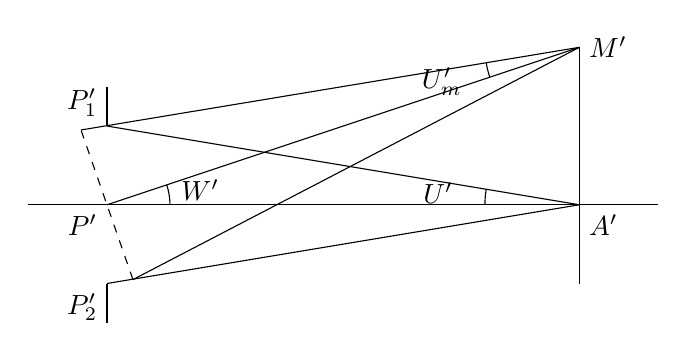
\begin{tikzpicture} 
	\coordinate [label=below left:$P'$] (A) at (-3,0);
	\coordinate [label=below right:$A'$] (B) at (3,0);
	\coordinate [label=right:$M'$] (C) at (3,2);
	\coordinate [label=above left:$P'_1$] (D) at (-3,1);
	\coordinate [label=below left:$P'_2$] (E) at (-3,-1);
	\draw[-] (-4,0) -- (4,0); 
	\draw[-] (A) -- (C); 
	\draw[-] (C) -- (3,-1); 
	\draw[-] (D) -- (-3,1.5); 
	\draw[-] (E) -- (-3,-1.5);
	\draw[-] (D) -- (B);
	\draw[-] (E) -- (B);
	\pic["$U'$", draw=black, -, angle eccentricity=1.5, angle radius=1.2cm]{angle=D--B--A};
	\pic["$W'$", draw=black, -, angle eccentricity=1.5, angle radius=0.8cm]{angle=B--A--C};
	\draw[-] (C) -- (-3.33,0.95);
	\draw[-,dashed] (-2.67,-0.95) -- (-3.33,0.95);
	\draw[-] (-2.67,-0.95) -- (C);
	\pic["$U'_m$", draw=black, -, angle eccentricity=1.5, angle radius=1.2cm]{angle=D--C--A};
	\end{tikzpicture}
	\caption{轴外像点的光照度}
	\label{fig:illuminance}
\end{figure}

如\figref{fig:illuminance} 所示,当物面亮度均匀时,有
\begin{equation}
E'_m=K\pi L\sin^2U'_m\bigg(\frac{n'}{n}\bigg)^2
\end{equation}
由于
\begin{equation}
\sin U'_m\approx\frac{P'P'_1\cos W'}{P'M'},\quad\sin U'\approx\frac{P'P'_1}{P'A'}
\end{equation}
得到
\begin{equation}
\frac{\sin U'_m}{\sin U'}\approx\frac{P'A'\cos W'}{P'M'}=\cos^2 W'
\end{equation}
所以
\begin{equation}
E'_M=E'\cos^4 W'
\end{equation}

\chapter{典型光学系统}

\section{眼睛}

眼睛作为显微镜和望远镜等目视光学仪器的接收器,它的构造级有关特性应在设计这类仪器时予以考虑。

\subsection{眼睛的构造}

\begin{figure}[htbp]
	\centering
	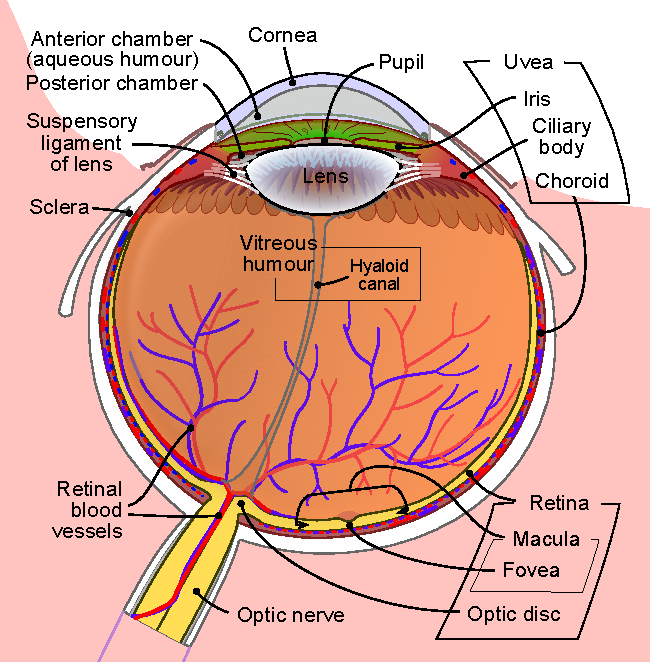
\includegraphics[width=0.5\textwidth]{structure-of-eye.pdf}
	\caption{人眼的内部构造}
	\label{fig:structure-of-eye}
\end{figure}

人眼呈球状,直径约$25\mathrm{mm}$,右眼的内部构造如\figref{fig:structure-of-eye} 所示。

眼球被一层坚韧的膜包围,前面突出的透明部分为\textbf{角膜},其余部分为\textbf{巩膜}。角膜后是充满折射率为$1.336$的透明液体的前室,前室的后壁为\textbf{虹彩膜},其中央部分有一圆孔,为\textbf{瞳孔}。虹膜之后是\textbf{水晶体},它是由多层薄膜构成的双凸透镜,各层折射率不同,内层约为$1.41$,外层约为$1.38$。水晶体后面是后室,也称为眼腔,内部充满折射率为$1.336$的透明胶装液体,称\textbf{玻状液}。后室的内壁与玻状液紧贴的部分是由视神经末梢组成的膜,称为\textbf{视膜},是眼球系统所成像的接收器,共有十层结构,前八层对光透明但不引起刺激,第九层是感光层,布满视神经细胞。第十层与脉络膜相连。\textbf{脉络膜}是网膜外包围着的一层黑色膜,吸收透过网膜的光线,避免感光器官受到强光的刺激。在视神经进入眼腔处附近的网膜上,有一个椭圆形区域,该区域内没有感光细胞,不产生视觉,称为\textbf{盲斑}。距盲斑中心$15^{\circ}30'$,在太阳穴方向有一椭圆区域e,大小为$1\mathrm{mm}$(水平方向)$\times0.8\mathrm{mm}$(垂直方向),称为\textbf{黄斑}。在黄斑中心有一$0.3\mathrm{mm}\times0.2\mathrm{mm}$的凹部,称为\textbf{中心凹}。中心凹密集了大量的感光细胞,是网膜上视觉最灵敏的区域。当眼睛观察外界物体时,会本能地转动眼球,使像成在中心凹上。因而称通过眼睛节点和中心凹的直线为眼睛的\textbf{视轴}。\footnote{本段对于眼睛结构的描述仅为简单的介绍,如需进一步了解请查阅相关文献。}

\begin{definition}{标准眼}{standard-eye}
	眼睛作为一个光学系统,其有关参数可由专门的仪器测出。根据大量的测量结果,定出了眼睛的各项光学常数,包括角膜、水状液、波状液和水晶体的折射率、各光学表面的曲率半径,以及各有关距离。满足这些光学常数值的眼睛称为标准眼。
\end{definition}

\begin{definition}{简约眼}{reduced-eye}
	为了作近似计算方便,可把标准眼简化为一个折射球面的模型,称为简约眼。简约眼的有关参数如下所示:
	\begin{enumerate}
		\item 折射面的曲率半径:$5.56\mathrm{mm}$
		\item 像方介质的折射率:$4/3=1.333$
		\item 视网膜的曲率半径:$9.7\mathrm{mm}$
	\end{enumerate}
	可算得简约眼的物方焦距为$-16.70\mathrm{mm}$,像方焦距为$22.26\mathrm{mm}$,光焦度为$59.88$屈光度。
\end{definition}

\subsection{眼睛的调节}
水晶体在睫状肌的作用下曲率可变,使不同远近的物体精确地成像在网膜上。当肌肉收缩时,水晶体曲率变大,可看清近物;肌肉放松时,水晶体曲率变小,可看清远物。眼睛的这种本能地改变水晶体光焦度以看清不同远近物体的功能称为\textbf{调节}。当肌肉完全放松时,眼睛所能看清的最远的点称为\textbf{远点};当肌肉收缩到最紧张状态时所能看清的最近点称为\textbf{近点}。分别以$p$和$r$表示近点和远点到眼睛物方主点的距离,则其倒数$P=1/p$和$R=1/r$就是近点和远点会聚度和屈光度数。二者之差以$A$表示,即
\begin{equation}
A=R-P
\end{equation}
称为调节范围或调节能力。

\subsubsection{正常眼}
正常眼的调节范围随年龄的变化而变化,年龄增大,肌肉收缩功能衰退,近点逐渐移远,调节范围减小。

\begin{definition}{明视距离}{distance-of-distinct-vision}
	明视距离是指正常眼在正常照明(约$50\mathrm{lx}$)下的正常阅读距离,国际规定为$250\mathrm{mm}$。
\end{definition}


\subsubsection{非正常眼}
非正常眼主要有以下几种:
\begin{enumerate}
	\item \textbf{近视眼}:远点在眼前的有限远处,$R<0$,眼球偏长,像方焦点位于网膜前,只有有限远处的物体才能成像在网膜上。\uline{校正方法:负光焦度眼镜}。
	\item \textbf{远视眼}:远点在眼镜之后,$R>0$,眼球偏短,像方焦点位于网膜后,只有会聚光束才能聚焦到网膜上。\uline{校正方法:正光焦度眼镜}。
	\item \textbf{散光眼}和\textbf{斜视眼}:水晶体位置不正、各个折射面曲率不正常或不对称。\uline{校正方法:前者用柱面透镜,后者用光楔}。
	\item \textbf{近视散光}:同时存在多种缺陷。
\end{enumerate}

\subsection{眼睛的适应}
人眼除了能随物体距离的改变而调节水晶体的曲率外,还能在不同亮暗条件下工作。眼睛所能感受到的光亮度变化范围为$10^{12}:1$。人从亮出到暗处发生暗适应,从暗处到亮处发生亮适应。

\subsection{眼睛的分辨率}
眼睛能分辨开两个很靠近的点的能力称为眼睛的\textbf{分辨率}。刚能分辨开的两个点对眼睛物方节点的张角称为眼睛的\textbf{极限分辨角}。分辨率与极限分辨角成反比。

入瞳为$D$的理想光学系统,其极限分辨角为
\begin{equation}
\varphi=\frac{1.22\lambda}{D}
\label{eq:limiting-angle-of-resolution}
\end{equation}
对$555$纳米的色光而言,若入瞳单位取毫米,将极限分辨角的单位取作秒,则有
\begin{equation}
\varphi''=\frac{140}{D}
\end{equation}

\begin{note}
	影响分辨率的因素:
	\begin{enumerate}
		\item 眼睛的分辨率随被观察物体的亮度和对比度而异。对比度一定,亮度越大分辨率越高;亮度一定,对比度越大分辨率越高。
		\item 照明光的光谱是影响分辨率的一个重要因素,由于眼睛有较大的色差,单色光的分辨率要比白光高,并以$555$nm的黄绿光为最高。
		\item 网膜上成像位置对分辨率有一定的影响,成像处于黄斑处分辨率最高。
	\end{enumerate}
\end{note}

\subsection{眼睛的瞄准精度}
在很多测量工作中,为了读数,常用某种标志对目标物进行对准或重合,例如用一根直线与另一直线重合。这种重合或对准的过程为\textbf{瞄准}。由于受到人眼分辨率的限制,二者完全重合是不可能的。偏离于完全重合的程度称为\textbf{瞄准精度}。瞄准精度随所选取的瞄准标志而异,最高时可达人眼分辨率的$1/5\sim1/10$。

\subsection{眼睛的立体视觉}
眼睛观察空间物体时,能区别它们的相对远近而具有立体视觉。通常,人们总以双眼观物。物在两眼中各自成像,两眼的视觉汇合到大脑产生但因的印象。物在两眼网膜上的像必须位于网膜的对应点,即相对于黄斑中心的同一侧,才有单像的印象。

\begin{figure}[htbp]
	\centering
	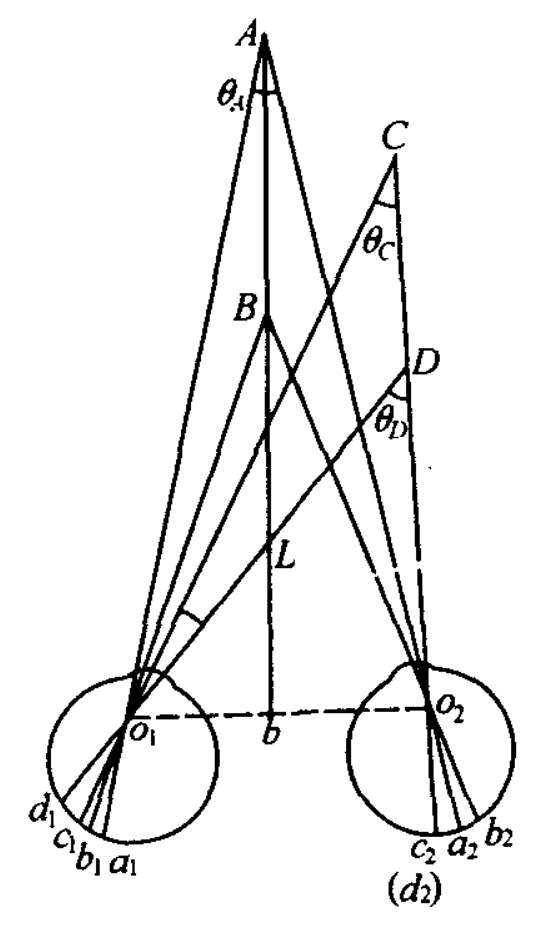
\includegraphics[width=0.3\textwidth]{two-eyes.png}
	\caption{双眼立体视觉}
	\label{fig:two-eyes}
\end{figure}

如\figref{fig:two-eyes} 所示,当两眼注视$A$点时,$A$点的像$a_1$和$a_2$位于黄斑中心,较近的B点在两网膜上的像$b_1$和$b_2$分别位于黄斑中心的外侧,不在对应点上,将明显感到是双像。此时凡在$\angle O_1AO_2$内的点都是成双像的。反之,当注视$B$点时,会感到较远的$A$点成双像。此外,当注视$A$点时,图中$C$点在两眼网膜上的像位于黄斑的同侧,将有单像的印象。

双眼视觉能够估计被观察物体的距离及分辨空间物体的相对远近,即双眼立体视觉。对于\figref{fig:two-eyes} 中不同远近的三个物点$A$、$B$、$C$,当两眼注视$A$点时,$A$在两眼网膜上的像$a_1$和$a_2$位于黄斑中位于黄斑中心,两视线的夹角$\angle O_1AO_2$称为视差角,即
\begin{equation}
\theta_A=\frac{b}{L}
\end{equation}
式中,$b$为两眼节点$O_1$和$O_2$的连线长度,称为基线长度;$L$为$A$到基线的距离。由此可见,不同远近的物体有不同的视差角。设另二点$C$和$D$位于直线$CDO_2$上,则它们在右眼中的像$c_2$和$d_2$重合,而左眼中的两个像$c_1$和$d_1$并不重合,其对节点$O_1$的张角即为$C$点和$D$点的视差角之差,即
\begin{equation}
\Delta\theta=\theta_D-\theta_C
\label{eq:parallax-angle-difference}
\end{equation}
称为立体视差。立体视差交大时,表示两物体的远近相差较大。当$\Delta\theta$小到某一限度时,人眼无法辨别两物体的远近。人眼刚好能够觉察的最小立体视差称为人眼的\textbf{体视锐度},用$\Delta\theta_0$表示。一般以$10''$作为体视锐度的极限值。

能分辨出不同远近的二点间的最小距离$\Delta L_0$称为体视阈值。对式(\ref{eq:parallax-angle-difference})进行微分,得
\begin{equation}
\Delta L_0=\frac{L^2}{b}\Delta\theta_0
\end{equation}
由该式可以看出,观察远物时,体视阈值很大,观察近物时,辨别其远近的能力强。如增大基线长度$b$和减小体视锐度$\Delta\theta_0$,体视圈半径$L_m$就可增大,体视阈值$\Delta L_0$就可减小,从而提高体视效果。

\begin{note}
成年人的双眼基线平均长度$b=65\mathrm{mm}$,当$\Delta\theta_0=10''$时,可导出双眼存在体视的距离$L_m=1350\mathrm{m}$,体视阈值$\Delta L_0=7.46\times10^{-4}\mathrm{m}$。
\end{note}

\section{放大镜}

对于目视光学仪器,其放大作用不能简单地以横向放大率来表征,而应代之以视觉放大率。
\begin{definition}{放大镜的放大率}{magnifier-magnification}
	通过放大镜看物体时,其像对眼睛张角的正切与直接看物体时,物体对眼睛张角的正切之比称为放大镜的放大率。
\end{definition}

\begin{figure}[htbp]
	\centering
	\begin{minipage}[t]{0.48\textwidth}
		\centering
		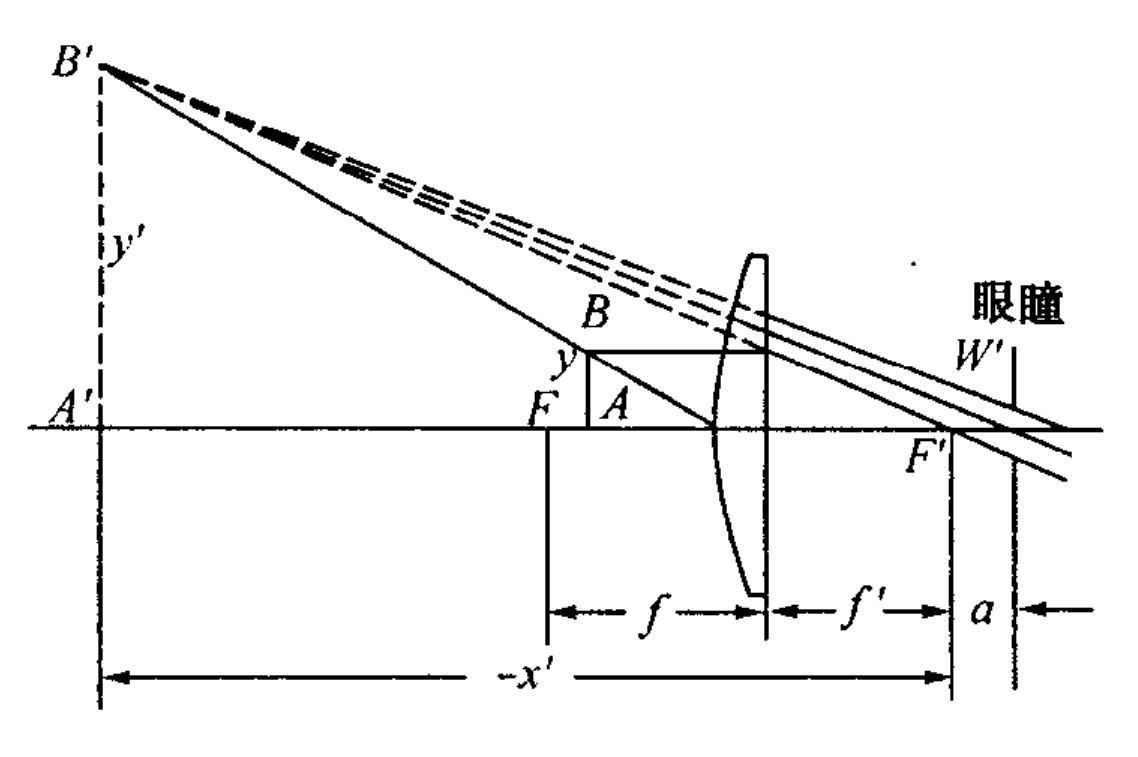
\includegraphics[width=1\textwidth]{magnifier-1.png}
		\caption{放大镜成像示意图}
		\label{fig:magnifier-1}
	\end{minipage}
	\quad
	\begin{minipage}[t]{0.48\textwidth}
		\centering
		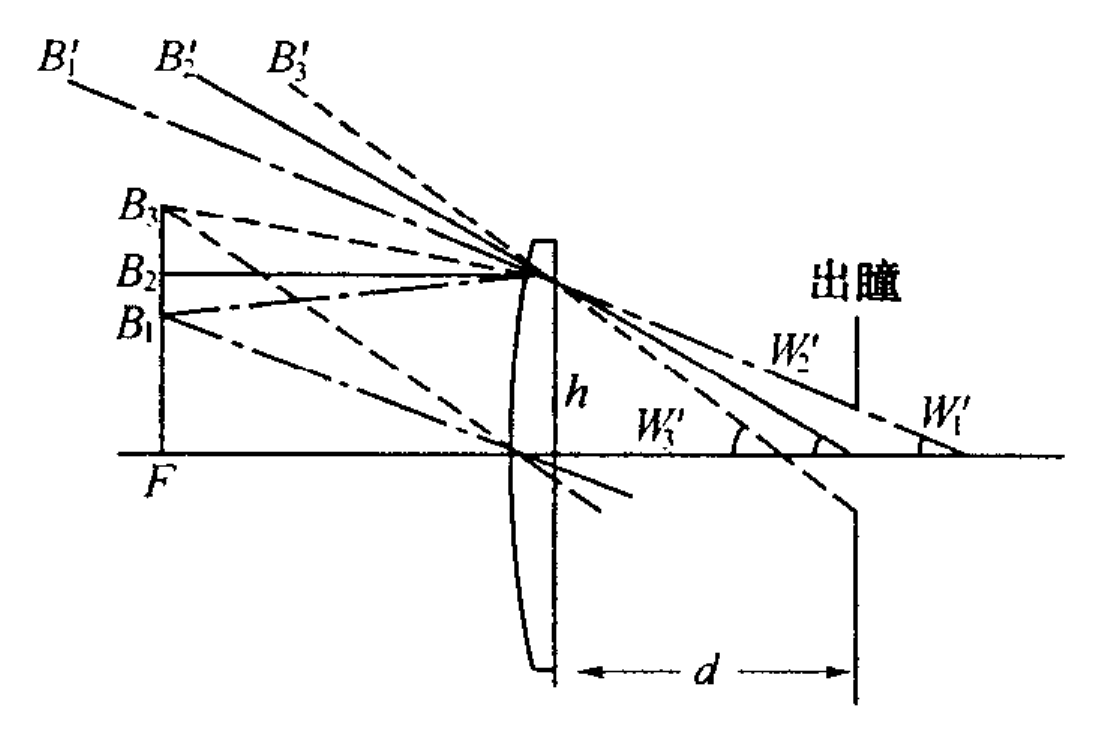
\includegraphics[width=1\textwidth]{magnifier-2.png}
		\caption{放大镜的渐晕}
		\label{fig:magnifier-2}
	\end{minipage}
\end{figure}

如\figref{fig:magnifier-1} 所示,放大镜将位于焦点以内的物$AB$在镜前明视距离处形成虚像$A'B'$,它对眼睛的张角为$W'$,有
\begin{equation}
\tan W'=\frac{y'}{-x'+a}
\end{equation}
而当眼睛直接于明视距离$250\mathrm{mm}$处观察物体时,对眼的张角为$W$,有
\begin{equation}
\tan W=\frac{y}{250}
\end{equation}
以$\tan W'/\tan W$表示放大镜的放大率$M$,并以$\beta=-x'/f'$代替$y'/y$,得
\begin{equation}
M=\frac{250}{f'}\frac{x'}{x'-a}
\end{equation}
由上式可见,放大镜的放大率除与焦距有关外,还与眼睛的位置有关,由于使用放大镜时,眼睛总位于像方焦点附近,$\alpha$相对于$x'$是一小量,于是
\begin{equation}
M=\frac{250}{f'}
\end{equation}
即放大镜的放大率仅由其焦距决定。焦距越短,放大率越大。

一般放大镜的直径比瞳孔直径大得多,物面上各点的成像光束是被眼瞳所限制的。眼瞳是孔径光阑,也是出瞳,放大镜是渐晕光阑。由于放大镜通光口径的限制,视场外围有渐晕而无明晰的边界。\figref{fig:magnifier-2} 画出了决定无渐晕成像范围的$B_1$点、$50\%$渐晕的$B_2$点和可能成像的最边缘点$B_3$,对应视场角分别为$W'_1$、$W'_2$和$W'_3$。由图可见
\begin{equation}
\tan W'_2=\frac{h}{d}
\end{equation}
同理易得出$\tan W'_1$和$\tan W'_3$的表达式。可见,放大镜的直径$2h$越大,眼睛越靠近放大镜,可见的视场就越大。如果以$50\%$渐晕点为界决定线视场,可导出
\begin{equation}
2y=\frac{500h}{Md}
\end{equation}
所以在放大镜的直径可眼瞳位置一定时,放大率越大,线视场越小。这就限制了放大镜的分辨率不能做得很大,一般不超过$15$倍。

\section{显微镜系统}
\subsection{显微镜概述}
显微镜的主光学系统由物镜和目镜两部分组成。\figref{fig:microscope-1} 为显微镜的成像原理图。显微镜的总放大率为物镜放大率$M_o$和目镜放大率$M_e$的乘积。这里
\begin{equation}
M_o=\beta=-\frac{\varDelta}{f'_o},\quad M_e=\frac{250}{f'_e}
\end{equation}
即
\begin{equation}
M=M_oM_e=-\frac{250\varDelta}{f'_of'_e}
\end{equation}
式中,$\varDelta=F'_oF_e$,为\textbf{光学筒长}。由此可见,显微镜的放大率与光学筒长成正比,与物镜和目镜的焦距成反比,且$M<0$,即对物体成倒像。

\begin{figure}[htbp]
	\centering
	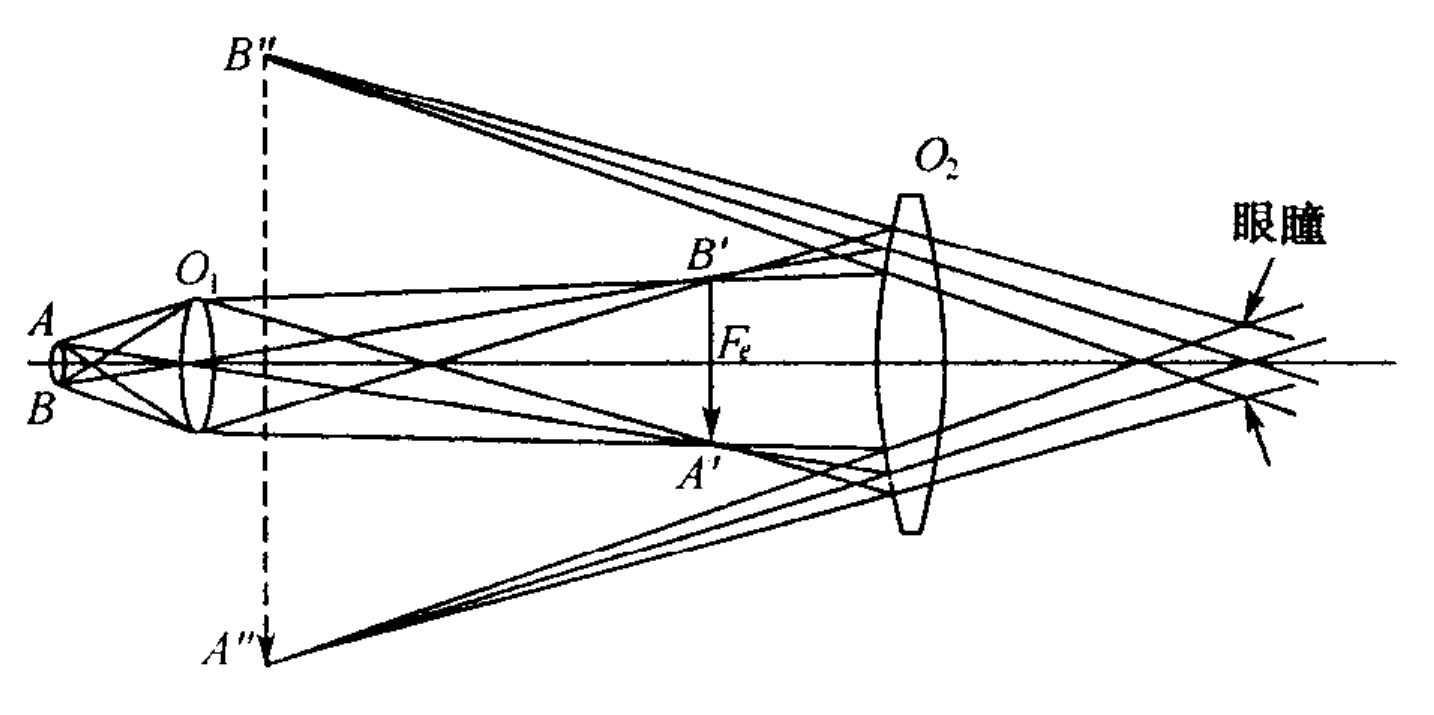
\includegraphics[width=0.6\textwidth]{microscope-1.png}
	\caption{显微镜成像原理图}
	\label{fig:microscope-1}
\end{figure}

\begin{definition}{机械筒长}{mechanical-tube-length}
	显微镜物镜和目镜的支撑面之间的距离$t_m$称为显微镜的机械筒长。我国标准为$160\mathrm{mm}$。
\end{definition}

\subsection{显微镜的孔径光阑}
对于单组低倍显微物镜,其镜框就是孔径光阑;对于多组透镜组成的复杂物镜,或以最后一组的透镜框作为孔径光阑,或在物镜的像方焦面上或其附近专设孔阑。这些孔阑的位置差异相对于光学筒长$\varDelta$是一个小量,因此孔阑被目镜所成的像,即显微镜的出射光瞳都在目镜的像方焦点之外近乎相同的地方,即距目镜像方焦点为$x'=f'^2_e/\varDelta$处。这正是整个显微镜的像方焦面位置。所以,在观察时眼瞳能与出瞳重合,且在更换物镜时不需要改变眼瞳的位置。

\begin{figure}[htbp]
	\centering
	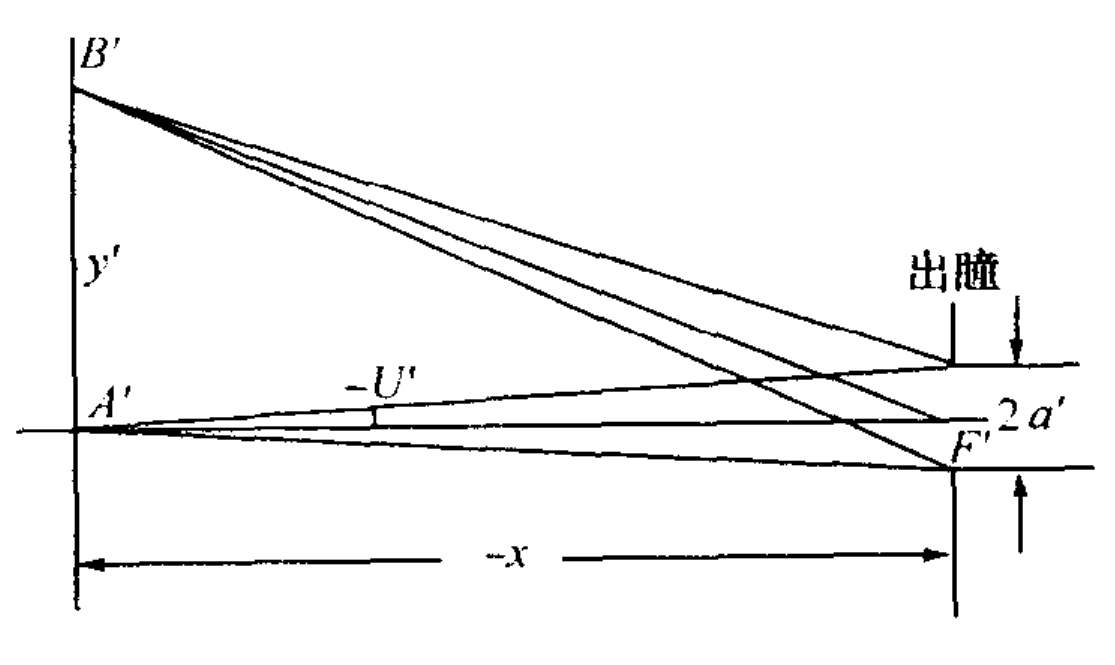
\includegraphics[width=0.6\textwidth]{microscope-2.png}
	\caption{显微镜像方成像}
	\label{fig:microscope-2}
\end{figure}

\figref{fig:microscope-2} 所示的是显微镜像方的成像光束,据此可以求出出瞳的大小为
\begin{equation}
a'=x'\tan U'\approx x'\sin U'
\end{equation}
利用正弦条件$n'y'\sin U'=ny\sin U$和横向放大率$\beta$的表达式,考虑到$n'=1$,可导出
\begin{equation}
a'=-f'n\sin U=-f'A
\end{equation}
式中,$A=n\sin U$称为显微镜物镜的\textbf{数值孔径},是显微镜的一个重要性能参数。引入显微镜的放大率,可得
\begin{equation}
a'=250\frac{A}{M}
\end{equation}
由此可见,显微镜的出瞳主要被其焦距或放大率所决定。高倍率时出瞳很小。

\subsection{显微镜的视场光阑}
在显微镜中间实像平面上有专设的视场光阑,其大小是物面上的可见范围(线视场)与物镜放大率的乘积。因此,高倍物镜只能看到物面上很小的范围,低倍物镜才有较大的视场。

\subsection{显微镜的景深}

\begin{figure}[htbp]
	\centering
	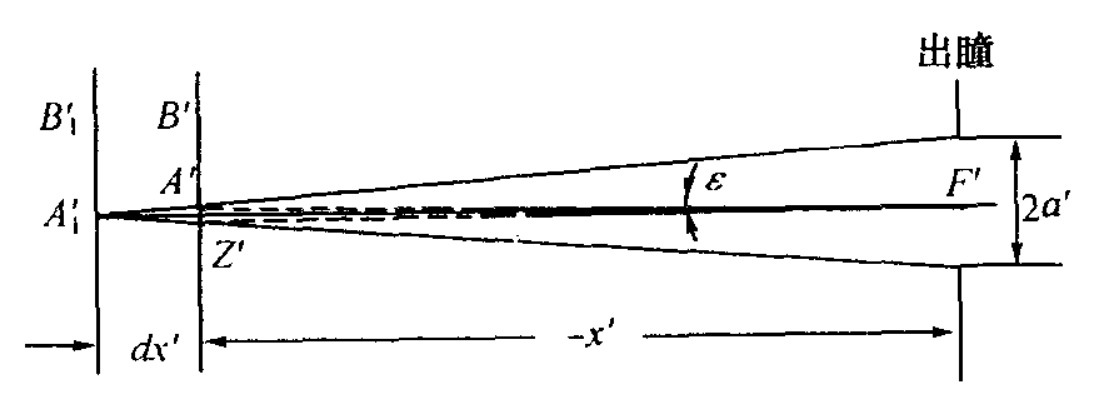
\includegraphics[width=0.6\textwidth]{microscope-depth-of-field.png}
	\caption{显微镜的景深}
	\label{fig:microscope-depth-of-field}
\end{figure}

如\figref{fig:microscope-depth-of-field} 所示,$A'B'$是对准平面被显微镜所成的像,即景像平面,$A'_1B'_1$是对准平面之前的物平面的像,与景深平面相距$\mathrm{d}x'$。设显微镜的出瞳与像方焦面重合,则$A'_1$点的成像光束被景深平面截得一弥散圆,其直径$Z'$由下式决定:
\begin{equation}
\frac{Z'}{2a'}=\frac{\mathrm{d}x'}{-x'+\mathrm{d}x'}
\end{equation}
若弥散圆对出瞳中心的张角不大于眼睛的极限分辨率$\varepsilon$,眼睛观察弥散圆即为点像。此时$2\mathrm{d}x'$即为像方能同时看清景象平面前后两像平面间的深度。因为有$|\mathrm{d}x'|\ll|x'|$,可以得到$2\mathrm{d}x'$的表达式。再利用轴向放大率$\alpha=n'\beta^2/n$,将此换算到物方,可得
\begin{equation}
2\mathrm{d}x'=\frac{nf'^2\varepsilon}{a'}
\end{equation}
再根据$a'=250A/M$以及$M=250/f'$,上式可表示为
\begin{equation}
2\mathrm{d}x'=\frac{250n\varepsilon}{MA}
\end{equation}
由此可见,显微镜的倍率越高,物镜的数值孔径越大,景深越小。

由于眼睛能在近点和远点间自行调节,景深将有所扩大。若在像空间中,近点和远点到眼瞳所在的出瞳面的距离为$p'$和$r'$,根据出瞳与显微镜的像方焦面重合可导出与此对应的物空间距离$p$和$r$,两者之差即为眼睛通过显微镜观察时的调节范围,有
\begin{equation}
r-p=-nf'^2\bigg(\frac{1}{r'}-\frac{1}{p'}\bigg)
\end{equation}
当$p'$和$r'$以米为单位时,括号内的值即为眼睛的调节范围$A$,单位为屈光度,即
\begin{equation}
r-p=-0.001nf'^2\overline{A}
\end{equation}

\subsection{显微镜的分辨率}

\begin{figure}[htbp]
	\centering
	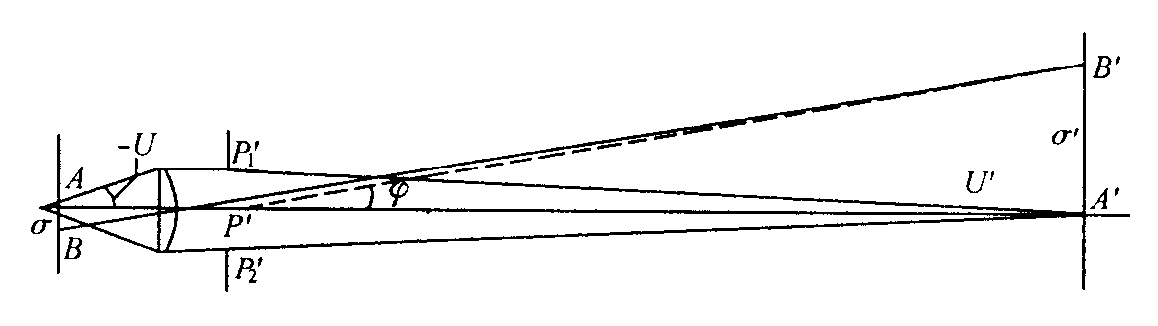
\includegraphics[width=0.8\textwidth]{resolution-of-microscope.png}
	\caption{显微镜分辨不同位置的两点}
	\label{fig:resolution-of-microscope}
\end{figure}

由瑞利判据可知,一个点的衍射像中心正好与另一点的衍射像第一暗环重合时,是光学系统刚好能分辨开这两点的最小界限。从波动光学的原理可知,自身发光的点被理想系统所成的衍射像,其第一暗环半径对出瞳中心所张的角,即正好能被此系统分辨得开的两个点的极限分辨角$\varphi$由式(\ref{eq:limiting-angle-of-resolution})决定,即$\varphi=1.22\lambda/D$。显微镜的分辨率以物面上能被物镜分辨开的两点之间的最小距离表示。如\figref{fig:resolution-of-microscope} 所示,对应的两像点之间的距离$\sigma'$应等于其中任一个衍射斑的第一暗环的半径,又因为像方孔径角很小,有
\begin{equation}
\sigma'=\varphi\cdot P'A'=\frac{0.61\lambda}{\tan U'}=\frac{0.61\lambda}{\sin U'}
\end{equation}

由于显微物镜满足正弦条件$n'\sigma'\sin U'=n\sigma\sin U$,且$n'=1$,所以得到最小分辨距为
\begin{equation}
\sigma=\frac{0.61\lambda}{n\sin U}=\frac{0.61\lambda}{A}
\end{equation}
对物体作斜照明,最小分辨角为
\begin{equation}
\sigma=\frac{0.5\lambda}{n\sin U}
\end{equation}
通过上述讨论可知,对于一定波长的色光,显微镜的分辨率在像差校正良好的情况下,完全被物镜的数值孔径所决定。数值孔径越大,分辨率越高。
\begin{property}
	显微镜的倍率越高,物镜的数值孔径越大,景深越小,分辨率越高。
\end{property}

\subsection{显微镜的放大率}
分别取$2'$和$4'$为人眼分辨角的下限和上限,人眼在明视距离处能分辨开两点的间距即为$\sigma$被显微镜放大以后的像,有
\begin{equation}
250\times2\times0.00029<\frac{0.5\lambda}{A}M<250\times4\times0.00029
\end{equation}
对于目视光学仪器,主色光波长为$0.00055\mathrm{mm}$,则
\begin{equation}
500A<M<1000A
\end{equation}
满足此公式的放大率称为显微镜的\textbf{有效放大率}。有效放大率由物镜的数值孔径决定,即数值孔径需与放大率相匹配。

\subsection{显微镜的物镜}

显微物镜有折射式、反射式和折反射式三类,绝大多数实用的物镜是折射式。折射式显微物镜可根据质量要求的不同而有不同的类型。
\begin{enumerate}
	\item 消色差物镜
	\begin{enumerate}
		\item 单组双胶合低倍物镜
		\item 李斯特型中倍物镜
		\item 阿米西型高倍物镜
		\item 阿贝浸液物镜
	\end{enumerate}
	\item 复消色差物镜
	\item 平场消色差物镜和平场复消色差物镜
\end{enumerate}

\subsection{显微镜的目镜}
显微镜中目镜相当于放大镜。\textbf{镜目距}是指目镜的出瞳到目镜最后一面的距离,为使眼瞳能和出瞳重合,镜目距不应小于$6\sim8\mathrm{mm}$。在目镜的物方焦面上设置视场光阑,其到目镜第一面的距离称谓目镜的\textbf{工作距离}。显微镜的目镜主要有:惠更斯目镜、冉斯登目镜、补偿目镜、平场目镜。

\subsection{显微镜的照明系统}
显微镜的照明系统主要有以下三类:
\begin{enumerate}
	\item 用透射光照明透明标本的照明系统
	\begin{enumerate}
		\item 临界照明
		
		\begin{figure}[htbp]
			\centering
			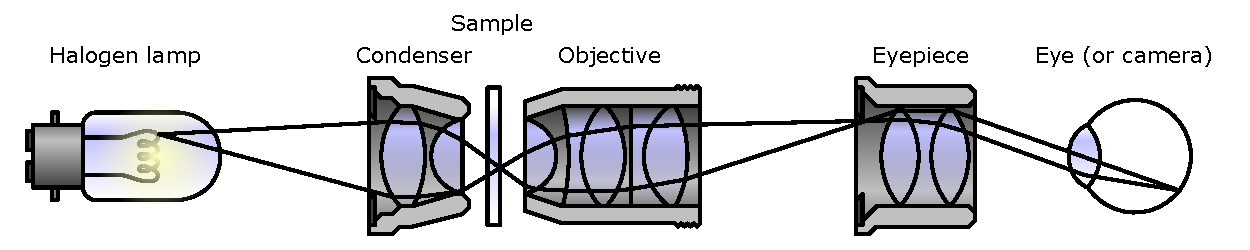
\includegraphics[width=0.9\textwidth]{critical-illumination.pdf}
			\caption{临界照明示意图}
			\label{fig:critical-illumination}
		\end{figure}
		
		光源通过照明系统或聚光镜成像于物面上,如\figref{fig:critical-illumination} 所示。其简化图如图所示(简化图待补充),图中的双点划线是从光源到物面再到像面的一对共轭关系,虚线是从光源光阑到物镜孔阑的另一对共轭关系。聚光镜的像方孔径角必须与物镜的物方孔径角相匹配,为此在聚光镜的物方焦面上或附近设置可变光阑。于是照明系统的出瞳正好与物镜的入瞳大致重合。
		\begin{note}
			临界照明的缺点是当光源的亮度不均匀或呈现明显的灯丝结构时,将会反映到物面上影响观察效果。
		\end{note}
		\item 柯拉照明
		
		\begin{figure}[htbp]
			\centering
			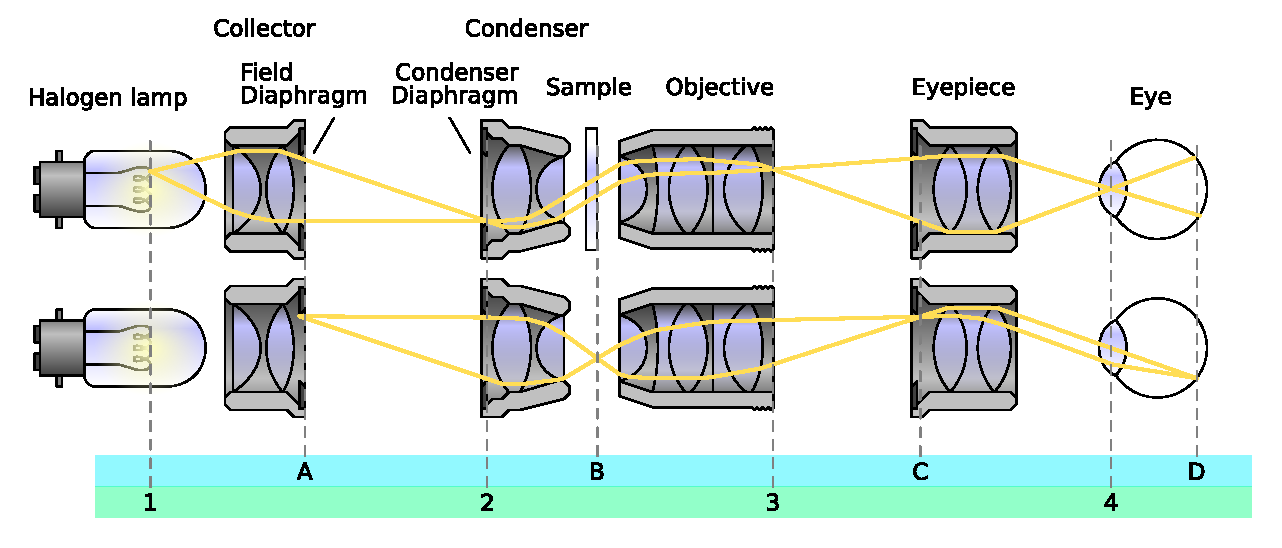
\includegraphics[width=0.9\textwidth]{kohler-illumination.pdf}
			\caption{柯拉照明示意图}
			\label{fig:kohler-illumination}
		\end{figure}
		
		光源成像在物镜入瞳面上,如\figref{fig:kohler-illumination} 所示。图中$A$、$B$、$C$、$D$是一组共轭关系,$1$、$2$、$3$、$4$是一组共轭关系。其简化图如图所示(简化图待补充),图中的虚线是从光源到物镜孔阑的一对共轭关系,双点划线是从光源光阑$J_1$到物面再到像面的另一对共轭关系。光源发出的光先经过一个前置透镜$L$成像于聚光镜前的可变光阑$J_2$上,聚光镜再将此光源像成在物镜的入瞳面上。在前置透镜后紧靠透镜处设置另一可变光阑,它被照明后具有均匀的亮度,并被聚光镜成像于物面上,使物面也得到均匀照明。调节光阑$J_2$可以使照明系统与不同数值孔径的物镜相匹配。调节光阑$J_1$可改变物面上的照明范围。
		\begin{note}
			对比两种照明方式可以发现,柯拉照明可以是临界照明将光源换成光源加前置物镜和光源光阑$J_1$,将光源通过前置物镜成像到$J_2$,$J_1$位于原临界照明的光源位置。
		\end{note}
		\begin{property}
			在照明系统和成像系统的合成系统中,成像系统的所有光都必然来自照明系统。这些光想要到达像面,必须通过照明系统和成像系统各自的瞳和窗。要使光传输的信息量不损失,任一光线都不能被照明系统或成像系统的任一光孔所拦截。那么只可能存在两种光瞳匹配关系,\uline{一种是照明系统的窗与成像系统的窗共轭,照明系统的瞳与成像系统的瞳共轭,这就是临界照明;另一种是照明系统的窗与成像系统的瞳共轭,照明系统的瞳与成像系统的窗共轭,这就是柯拉照明}。
		\end{property}
	\end{enumerate}
	\item 非透明物体的照明系统
	
	光必须从侧面或者正面照明。
	\item 用暗视场观察微小质点的照明方法
	
	用暗视场方法可以观察到超显微质点,即小于显微镜分辨极限的质点。
\end{enumerate}

\section{望远镜系统}
\subsection{望远镜的一般特性}
望远镜系统是一种使入射的平行光束仍保持平行射出的光学系统。最简单的望远镜系统必须由两个光组组成。前一光组的像方焦点与后一光组的物方焦点重合,即光学间隔$\varDelta=0$。光组$L_1$朝向物体,为望远镜的物镜;光组$L_2$为目镜。具有正光焦度目镜的系统为\textbf{开普勒望远镜},具有负光焦度目镜的系统为\textbf{伽利略望远镜}。

\begin{figure}[htbp]
	\centering
	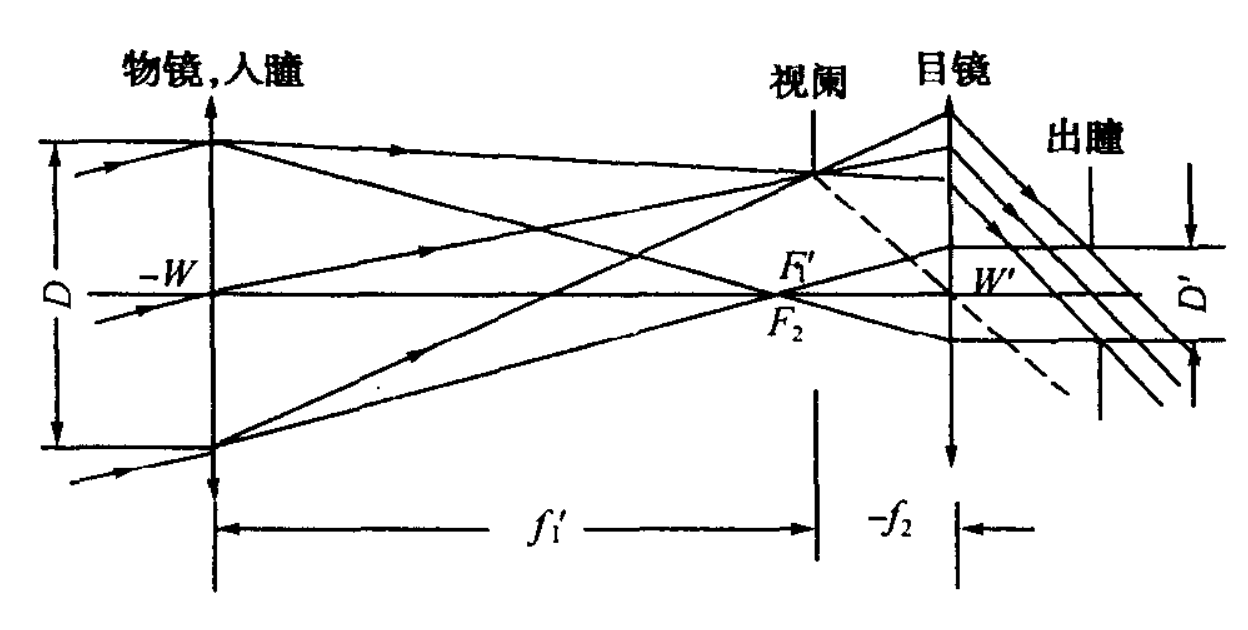
\includegraphics[width=0.7\textwidth]{kepler-telescope.png}
	\caption{开普勒望远镜系统}
	\label{fig:kepler-telescope}
\end{figure}

如\figref{fig:kepler-telescope} 所示为光束经开普勒望远镜系统的光路,物镜的通光孔径限制了轴上点的成像光束,是系统的孔径光阑和入瞳,出瞳是物镜的通光孔被目镜所成的像,应在目镜的像方焦点之外,能与观察者的眼瞳重合。

\begin{definition}{望远镜的放大率}{magnification-of-telescope}
	眼睛通过望远镜观察时,物体的像对眼睛张角的正切与眼睛直接看该物体时,物体对眼睛张角的正切之比,即为望远镜的放大率,以$\varGamma$表示。由于物方、像方都位于无穷远,此放大率即为系统本身的像方视场角与物方视场角的正切值比,有
	\begin{equation}
	\varGamma=\frac{\tan W'}{\tan W}=-\frac{f'_1}{f'_2}=\frac{D}{D'}
	\label{eq:visual-magnification}
	\end{equation}
	所以,望远镜的放大率还可表示为物镜焦距与目镜焦距之比、入瞳直径与出瞳直径之比。由式(\ref{eq:visual-magnification})可知,开普勒望远镜成倒像,伽利略望远镜成正像。
\end{definition}

\begin{property}
由视觉放大率公式(\ref{eq:visual-magnification})可知:
\begin{enumerate}
	\item 当物镜的焦距大于目镜的焦距时,望远镜有视觉放大作用;
	\item 当目镜的焦距一定时,倍率越高,物镜的焦距越长,导致望远镜的长度越大;
	\item 当像方视场角$W'$一定时,倍率越大,物方视场越小;
	\item 当入瞳直径一定时,倍率越大,出瞳直径越小,当出瞳小于眼瞳时,视见像的光强度下降。
\end{enumerate}
\end{property}

\begin{definition}{望远镜的正常放大率}{normal-magnification-of-telescope}
	当望远镜的入瞳直径为$D$时,它能分辨的远处两点对入瞳中心的最小张角为$\varphi''=140/D$,为充分利用物镜的分辨率,望远镜应把此角度放大到能为眼睛所分辨的程度,因此要求$\varGamma\varphi''\geqslant60''\sim70''$,即
	\begin{equation}
	\varGamma\geqslant0.5D
	\end{equation}
	式中,$D$的单位为毫米。按照此式确定的放大率称为望远镜的正常放大率,对应的出瞳直径为$2\mathrm{mm}$,和白天光亮条件下眼瞳直径相当。
\end{definition}
较多情况下按仪器用途确定的放大率大于正常放大率。若通过望远镜瞄准,则瞄准误差应为
\begin{equation}
\Delta\alpha''=\frac{\alpha''}{\varGamma}
\end{equation}
式中$\alpha''$为肉眼瞄准误差,由此可见增大倍率可提高瞄准镜度。

\subsection{望远镜的主观亮度}
\begin{definition}{主观亮度}{subjective-luminance}
	眼睛观物时,成在视网膜上的像对感光神经末梢的作用所引起的视觉刺激程度,称为主观亮度。眼睛直接观物时感知的像的明亮程度称为肉眼的主观亮度;通过望远镜观察时感知的像的明亮程度称为望远镜的主观亮度。
\end{definition}

\subsubsection{点物或点光源的像}
	
像的主观亮度仅决定于进入眼睛的光通量。当通过望远镜观察点光源时,能进入望远镜的光通量$\varPhi_T$被入瞳直径$D$决定,用人眼直接观察时,能进入眼瞳的光通量$\varPhi_e$由眼瞳的直径$D_e$决定。若眼瞳直径$D_e$大于望远镜的出瞳直径$D'$,所有射入望远镜的光通量全部都能进入眼睛,因此点像的主观亮度要比肉眼观察时大。其相对主观亮度,即两种情况下的光通量之比为:
\begin{equation}
\frac{\varPhi_T}{\varPhi_e}=k\frac{D^2}{D^2_e}
\label{eq:relative-subjective-luminance-1}
\end{equation}
其中,$k$为望远镜的透射率。若望远镜的出瞳直径$D'$与眼瞳直径$D_e$相等,此时有$D=\varGamma D_e$,则相对主观亮度为
\begin{equation}
\frac{\varPhi_T}{\varPhi_e}=k\varGamma^2
\label{eq:relative-subjective-luminance-2}
\end{equation}
若出瞳大于眼瞳,则进入望远镜的光通量不能全部进入眼瞳,眼睛便成为整个光学系统的出瞳,入瞳直径应为$\varGamma D_e$,此时同样可得公式(\ref{eq:relative-subjective-luminance-2})。
\begin{property}
	望远镜的物镜口径一定时,倍率越高,相对主观亮度越大,但倍率高到使出瞳不大于眼瞳时,即为定值。当望远镜的倍率和眼瞳直径一定时,物镜的直径越大,相对主观亮度也越大。
\end{property}
观察天空中微弱发光的星星时,应使用倍率高,物镜孔径大的天文望远镜。
	
\subsubsection{观察有限大小物体}
	
有限大小物体的像的主观亮度由网膜上的照度决定。通过望远镜观察的物体与人眼直接观察同一物体在视网膜上像面积之比为$\varGamma^2$,由$E=\varPhi/S$与式(\ref{eq:relative-subjective-luminance-1})可得观察有限大小物体的相对主观亮度为
\begin{equation}
\frac{E_T}{E_e}=k\bigg(\frac{D'}{D_e}\bigg)^2
\end{equation}
上式的值不可能大于$k$,因此用望远镜观察有限大小的物体时,主观亮度总比用肉眼观察时低。所以在黄昏或夜间使用的望远镜因眼瞳较大,应有较大的出瞳。望远镜的倍率越高,出瞳越小,当用于天文观察时,作为点光源的星星,其相对主观亮度很大,而作为背景的天空,相对主观亮度很小,因此在白天,利用高倍天文望远镜可以看见明亮天空中的星星。

\subsection{望远镜的光束限制}

伽利略望远镜和开普勒望远镜具有不同的光束限制。

\figref{fig:galileo-telescope} 所示的是伽利略望远镜物方的入瞳和物镜、像方的出瞳和渐晕光阑的像。根据几何关系可以得出无渐晕、$50\%$渐晕的视场角,后者的正切为
\begin{equation}
\tan W=\frac{D}{2l}=\frac{D}{2\varGamma(f'_1+f'_2+\varGamma l'_p)}
\end{equation}
式中,$D$为物镜的直径,$l'_p$为出瞳距。由此可见,伽利略望远镜的倍率越高,视场越小,视场还随眼睛远离目镜而变小。
\begin{figure}[htbp]
	\centering
	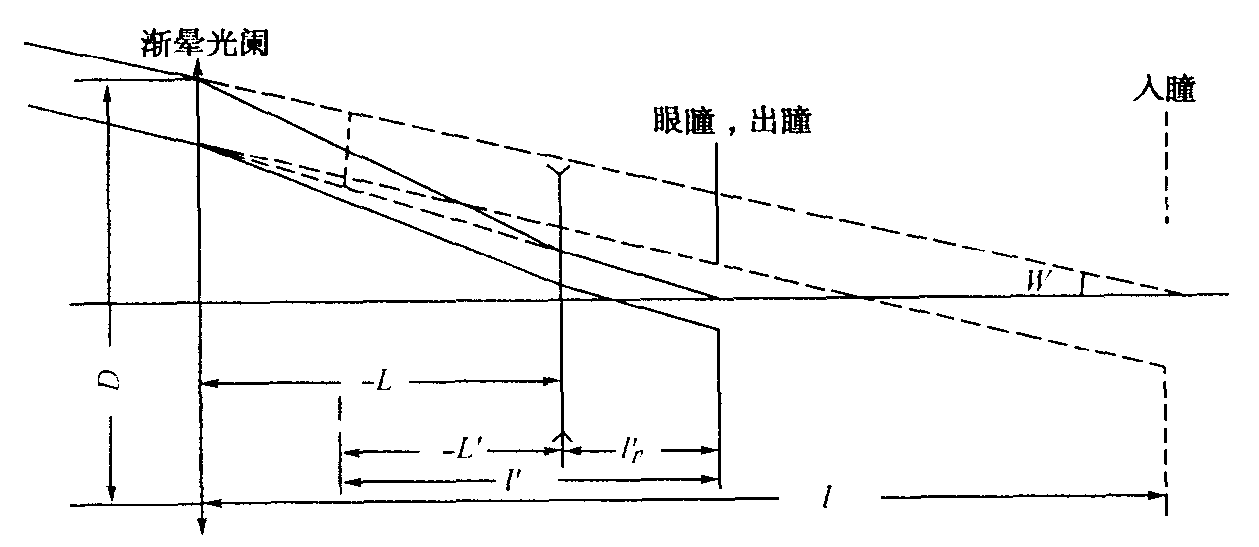
\includegraphics[width=0.8\textwidth]{galileo-telescope.png}
	\caption{伽利略望远镜系统}
	\label{fig:galileo-telescope}
\end{figure}
\begin{note}
	伽利略望远镜的优劣:伽利略望远镜的优点在于结构简单,筒长短,轻便,光能损失少,成正像。但伽利略望远镜没有中间的实像面,不能设置分划板作瞄准和定位。	
\end{note}

开普勒望远镜的目镜为正光焦度,在物镜和目镜之间具有中间实像平面,可以在其上设置视阑,安装分划板,作瞄准、定位和测量之用。分划板是在磨光的玻璃片上刻以分划标志的光学零件,其通光口径就是视阑的直径,有
\begin{equation}
D_F=2f'\tan W
\end{equation}
通过开普勒望远镜观察物体时,有明晰的视场边界。为了在大相对孔径和大视场的情况下不致使目镜的直径太大,并减少目镜斜光束像差的有害影响,可适当减小目镜的口径而允许轴外点存在$50\%$的渐晕。此时\figref{fig:kepler-telescope} 中主光线以上部分光束将被目镜限制而不能通过。
\begin{note}
	开普勒望远镜成倒像,只适用于天文观测或专设目标的瞄准和测量,为了便于观察可加入转像系统。结构上比伽利略望远镜复杂。	
\end{note}

\subsection{望远镜的物镜}
望远镜物镜只需要对轴上点校正色差、球差和对近轴点校正彗差,轴外像差可不予考虑,其结构比较简单。
\begin{enumerate}
	\item 折射式望远镜物镜:双胶合物镜、双分离物镜、三分离物镜、内调焦物镜
	\item 反射式望远镜物镜:卡塞格林系统、格利果里系统
	\item 折反射式望远镜物镜:施密特物镜、马克苏托夫物镜、无光焦度的双透镜与球面卡氏系统的组合
\end{enumerate}

\subsection{望远镜的目镜}
用于瞄准和测量的望远镜在其视阑平面上设置有分划板。为使屈光不正的观察者能看清分划板,目镜应能做视度调节。若要求视度的调节范围为$\pm N$个屈光度,目镜相对于分划板的调焦量$\Delta l$应为
\begin{equation}
\Delta l=\pm\frac{Nf'^2_2}{1000}(\mathrm{mm})
\end{equation}
式中,$f'_2$为目镜的焦距,以毫米计,一般仪器中,要求$N=\pm5$屈光度。目镜的工作距离应大于$\Delta l$。常用的目镜有:冉斯登目镜、凯涅尔目镜、对称式目镜、阿贝无畸变目镜、爱弗尔目镜。

\subsection{转像系统与场镜}
实际应用中使用的望远镜都是利用转像系统使倒像转成正像的开普勒望远镜。这种望远镜称为地上望远镜,转像系统为棱镜系统或透镜系统。
\subsubsection{棱镜转像系统}
用单块屋脊棱镜或由普通棱镜组合起来的棱镜系统,均能达到使像相对于物体在上下和左右两个方向都倒转过来的目的。详见第 \ref{sect:reflecting-prism} 节。

\subsubsection{透镜转向系统}
\begin{definition}{透镜转向系统}{lens-steering-system}
	设在物镜的实像平面后面,使倒像再一次倒转成为正像的透镜系统称为透镜转像系统。
\end{definition}
透镜转向系统有两种形式,如\figref{fig:lens-steering-system-1} 和\figref{fig:lens-steering-system-2} 所示。
\begin{figure}[htbp]
	\centering
	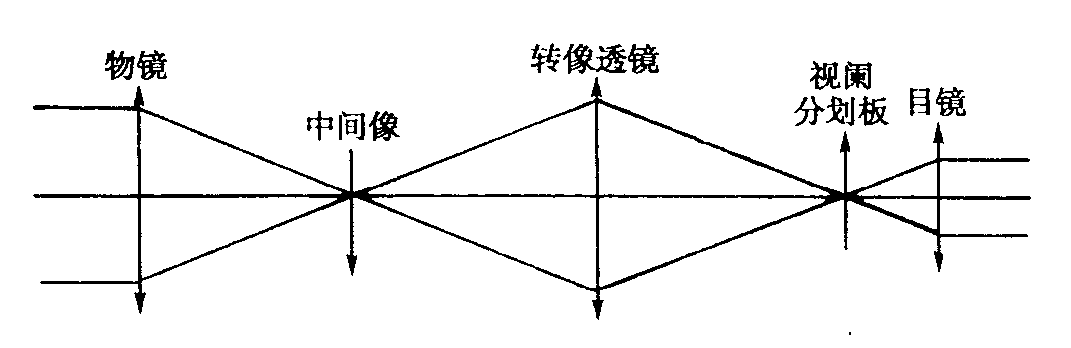
\includegraphics[width=0.7\textwidth]{lens-steering-system-1.png}
	\caption{透镜转向系统(单组)}
	\label{fig:lens-steering-system-1}
\end{figure}
\begin{figure}[htbp]
	\centering
	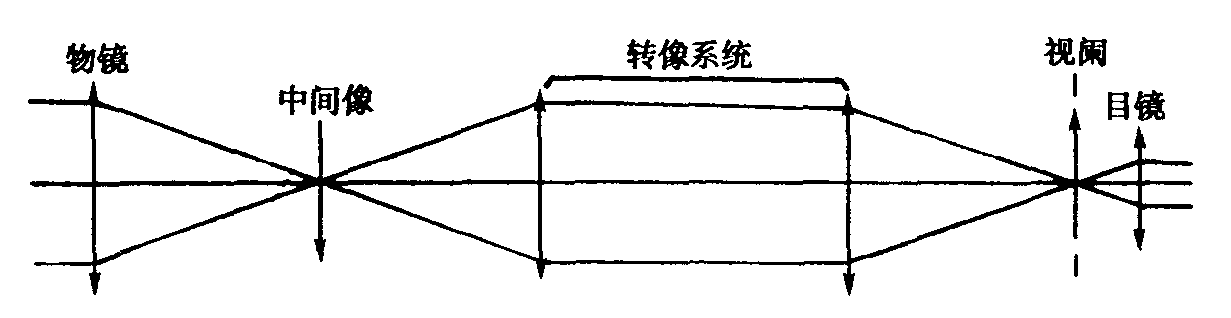
\includegraphics[width=0.8\textwidth]{lens-steering-system-2.png}
	\caption{透镜转向系统(双组)}
	\label{fig:lens-steering-system-2}
\end{figure}

\subsubsection{场镜}
如果只是简单地加入透镜转向系统,轴外点成像光束在转像镜组上的入射高度会大大增加,导致视场较大,绝大部分光线不能通过转像系统。为此,可以在中间实像平面上加一适当光焦度的透镜,使望远镜的光瞳与转像系统的光瞳共轭,使轴外光束折向转像镜组。这种加于中间相面上或附近的透镜称为场镜,它的光焦度对系统的总光焦度并无贡献,不影响轴上点光束和系统的放大率。

根据像差理论可知,位于像面上的场镜除了产生匹兹凡和以及由此引起的畸变外,不产生其他像差。因此场镜都使用单透镜,并且在不需由它来改变畸变时,都采用平凹透镜。

\section{摄影光学系统}

\section{放映系统}


\chapter{像差理论}



\part{物理光学}

\part{光电子学}

%\bibliography{reference}
\appendix
\chapter{几何光学习题解答}
\begin{enumerate}[itemsep=1.5ex]

	\item 备用附录
	
\end{enumerate}

\end{document}